\section{Floats in general}
Just ignore the position of floats until that is really the last ting for you to change.

\section{Figures folder structure and formats}

By organizing your figures into folders, like
./figs/pics/\footnote{Pictures, examples, etc}, ./figs/pdf/, ./figs/pgf/, ./figs/png/, ./figs/tikz/, and add
    
    \begin{minted}{latex}
    \graphicspath{{./figs/pics/}{./figs/tikz/}}
    \end{minted}

    to your preamble. This will tell tex to look for figures in ./figs/pics/ and ./figs/tikz/.
    You can then either supply

    \begin{minted}{latex}
        \includegraphics{example_1}
    \end{minted}

    where tex will look for some\_fig in ./figs/pics/ and ./figs/tikz/, or provide a full/relative path, as

    \begin{minted}{latex}
        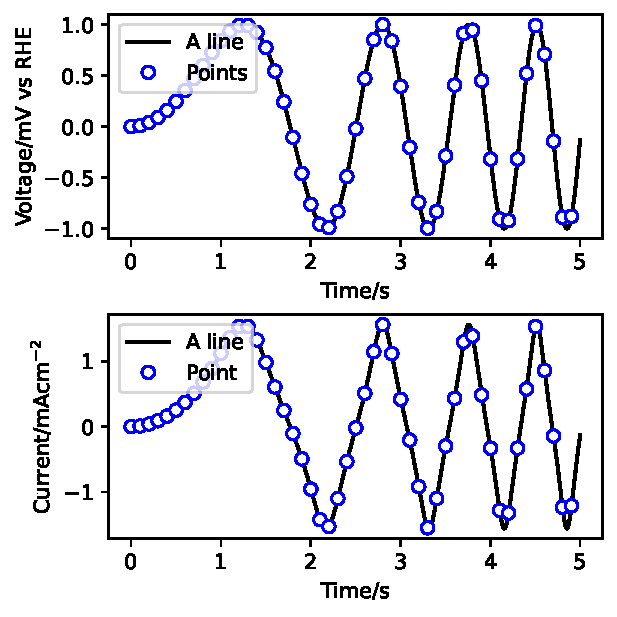
\includegraphics{./figs/pdf/example_1}
    \end{minted}

            

\Cref{figures:fig:example:1} was included with 


\begin{minted}{latex}
    \begin{figure}[htbp]
        \includegraphics[width=0.7\textwidth]{example_1}
        \caption{Example figure included without file extension and file path.}
        \label{figures:fig:example:1}
    \end{figure}
\end{minted}


\begin{figure}[htbp]
    \includegraphics[width=0.7\textwidth]{example_1}
    \caption{Example figure included without file extension and file path.}
    \label{figures:fig:example:1}
\end{figure}

    You can still specify the absolute path if you like, but the abov example makes changing from .tikz to .png really easy. 
    
    In \cref{figures:fig:example:2}, the absolute paths are specified, and the code looks like

    \begin{minted}{latex}
        \begin{figure}
            \begin{subfigure}[t]{0.45\textwidth}
            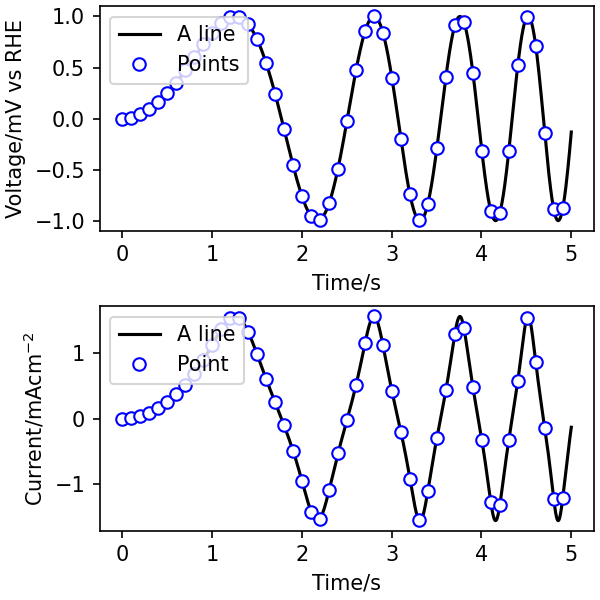
\includegraphics[width=\linewidth]{./figs/png/example_1}
            \caption{.png}
            \label{figures:fig:exmaple:2:png}
            \end{subfigure}
            \hfill
            \begin{subfigure}[t]{0.45\textwidth}
            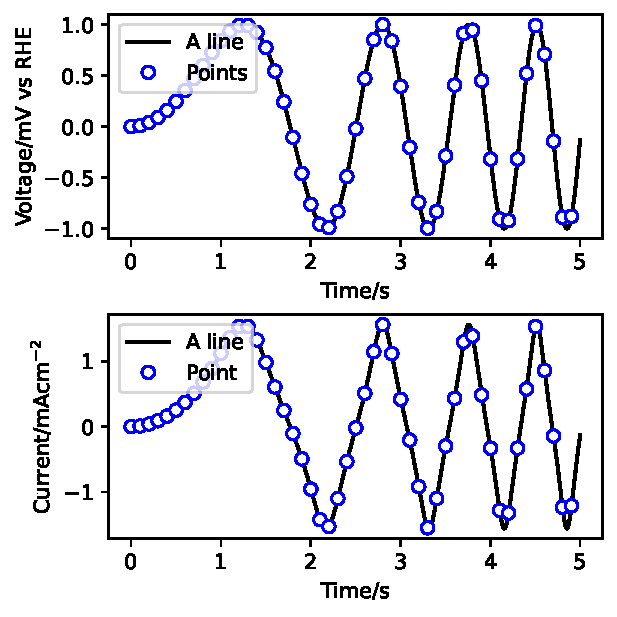
\includegraphics[width=\linewidth]{./figs/pdf/example_1}
            \caption{.pdf}
            \label{figures:fig:exmaple:2:pdf}
            \end{subfigure}
            %
            \begin{subfigure}[t]{0.45\textwidth}
            \resizebox*{\linewidth}{!}{%% Creator: Matplotlib, PGF backend
%%
%% To include the figure in your LaTeX document, write
%%   \input{<filename>.pgf}
%%
%% Make sure the required packages are loaded in your preamble
%%   \usepackage{pgf}
%%
%% Also ensure that all the required font packages are loaded; for instance,
%% the lmodern package is sometimes necessary when using math font.
%%   \usepackage{lmodern}
%%
%% Figures using additional raster images can only be included by \input if
%% they are in the same directory as the main LaTeX file. For loading figures
%% from other directories you can use the `import` package
%%   \usepackage{import}
%%
%% and then include the figures with
%%   \import{<path to file>}{<filename>.pgf}
%%
%% Matplotlib used the following preamble
%%   \usepackage{fontspec}
%%   \setmainfont{DejaVuSerif.ttf}[Path=\detokenize{C:/Users/kristian/anaconda3/lib/site-packages/matplotlib/mpl-data/fonts/ttf/}]
%%   \setsansfont{DejaVuSans.ttf}[Path=\detokenize{C:/Users/kristian/anaconda3/lib/site-packages/matplotlib/mpl-data/fonts/ttf/}]
%%   \setmonofont{DejaVuSansMono.ttf}[Path=\detokenize{C:/Users/kristian/anaconda3/lib/site-packages/matplotlib/mpl-data/fonts/ttf/}]
%%
\begingroup%
\makeatletter%
\begin{pgfpicture}%
\pgfpathrectangle{\pgfpointorigin}{\pgfqpoint{4.000000in}{4.000000in}}%
\pgfusepath{use as bounding box, clip}%
\begin{pgfscope}%
\pgfsetbuttcap%
\pgfsetmiterjoin%
\definecolor{currentfill}{rgb}{1.000000,1.000000,1.000000}%
\pgfsetfillcolor{currentfill}%
\pgfsetlinewidth{0.000000pt}%
\definecolor{currentstroke}{rgb}{1.000000,1.000000,1.000000}%
\pgfsetstrokecolor{currentstroke}%
\pgfsetdash{}{0pt}%
\pgfpathmoveto{\pgfqpoint{0.000000in}{0.000000in}}%
\pgfpathlineto{\pgfqpoint{4.000000in}{0.000000in}}%
\pgfpathlineto{\pgfqpoint{4.000000in}{4.000000in}}%
\pgfpathlineto{\pgfqpoint{0.000000in}{4.000000in}}%
\pgfpathlineto{\pgfqpoint{0.000000in}{0.000000in}}%
\pgfpathclose%
\pgfusepath{fill}%
\end{pgfscope}%
\begin{pgfscope}%
\pgfsetbuttcap%
\pgfsetmiterjoin%
\definecolor{currentfill}{rgb}{1.000000,1.000000,1.000000}%
\pgfsetfillcolor{currentfill}%
\pgfsetlinewidth{0.000000pt}%
\definecolor{currentstroke}{rgb}{0.000000,0.000000,0.000000}%
\pgfsetstrokecolor{currentstroke}%
\pgfsetstrokeopacity{0.000000}%
\pgfsetdash{}{0pt}%
\pgfpathmoveto{\pgfqpoint{0.657765in}{2.463273in}}%
\pgfpathlineto{\pgfqpoint{3.958330in}{2.463273in}}%
\pgfpathlineto{\pgfqpoint{3.958330in}{3.958330in}}%
\pgfpathlineto{\pgfqpoint{0.657765in}{3.958330in}}%
\pgfpathlineto{\pgfqpoint{0.657765in}{2.463273in}}%
\pgfpathclose%
\pgfusepath{fill}%
\end{pgfscope}%
\begin{pgfscope}%
\pgfsetbuttcap%
\pgfsetroundjoin%
\definecolor{currentfill}{rgb}{0.000000,0.000000,0.000000}%
\pgfsetfillcolor{currentfill}%
\pgfsetlinewidth{0.803000pt}%
\definecolor{currentstroke}{rgb}{0.000000,0.000000,0.000000}%
\pgfsetstrokecolor{currentstroke}%
\pgfsetdash{}{0pt}%
\pgfsys@defobject{currentmarker}{\pgfqpoint{0.000000in}{-0.048611in}}{\pgfqpoint{0.000000in}{0.000000in}}{%
\pgfpathmoveto{\pgfqpoint{0.000000in}{0.000000in}}%
\pgfpathlineto{\pgfqpoint{0.000000in}{-0.048611in}}%
\pgfusepath{stroke,fill}%
}%
\begin{pgfscope}%
\pgfsys@transformshift{0.807791in}{2.463273in}%
\pgfsys@useobject{currentmarker}{}%
\end{pgfscope}%
\end{pgfscope}%
\begin{pgfscope}%
\definecolor{textcolor}{rgb}{0.000000,0.000000,0.000000}%
\pgfsetstrokecolor{textcolor}%
\pgfsetfillcolor{textcolor}%
\pgftext[x=0.807791in,y=2.366051in,,top]{\color{textcolor}\sffamily\fontsize{10.000000}{12.000000}\selectfont 0}%
\end{pgfscope}%
\begin{pgfscope}%
\pgfsetbuttcap%
\pgfsetroundjoin%
\definecolor{currentfill}{rgb}{0.000000,0.000000,0.000000}%
\pgfsetfillcolor{currentfill}%
\pgfsetlinewidth{0.803000pt}%
\definecolor{currentstroke}{rgb}{0.000000,0.000000,0.000000}%
\pgfsetstrokecolor{currentstroke}%
\pgfsetdash{}{0pt}%
\pgfsys@defobject{currentmarker}{\pgfqpoint{0.000000in}{-0.048611in}}{\pgfqpoint{0.000000in}{0.000000in}}{%
\pgfpathmoveto{\pgfqpoint{0.000000in}{0.000000in}}%
\pgfpathlineto{\pgfqpoint{0.000000in}{-0.048611in}}%
\pgfusepath{stroke,fill}%
}%
\begin{pgfscope}%
\pgfsys@transformshift{1.407893in}{2.463273in}%
\pgfsys@useobject{currentmarker}{}%
\end{pgfscope}%
\end{pgfscope}%
\begin{pgfscope}%
\definecolor{textcolor}{rgb}{0.000000,0.000000,0.000000}%
\pgfsetstrokecolor{textcolor}%
\pgfsetfillcolor{textcolor}%
\pgftext[x=1.407893in,y=2.366051in,,top]{\color{textcolor}\sffamily\fontsize{10.000000}{12.000000}\selectfont 1}%
\end{pgfscope}%
\begin{pgfscope}%
\pgfsetbuttcap%
\pgfsetroundjoin%
\definecolor{currentfill}{rgb}{0.000000,0.000000,0.000000}%
\pgfsetfillcolor{currentfill}%
\pgfsetlinewidth{0.803000pt}%
\definecolor{currentstroke}{rgb}{0.000000,0.000000,0.000000}%
\pgfsetstrokecolor{currentstroke}%
\pgfsetdash{}{0pt}%
\pgfsys@defobject{currentmarker}{\pgfqpoint{0.000000in}{-0.048611in}}{\pgfqpoint{0.000000in}{0.000000in}}{%
\pgfpathmoveto{\pgfqpoint{0.000000in}{0.000000in}}%
\pgfpathlineto{\pgfqpoint{0.000000in}{-0.048611in}}%
\pgfusepath{stroke,fill}%
}%
\begin{pgfscope}%
\pgfsys@transformshift{2.007996in}{2.463273in}%
\pgfsys@useobject{currentmarker}{}%
\end{pgfscope}%
\end{pgfscope}%
\begin{pgfscope}%
\definecolor{textcolor}{rgb}{0.000000,0.000000,0.000000}%
\pgfsetstrokecolor{textcolor}%
\pgfsetfillcolor{textcolor}%
\pgftext[x=2.007996in,y=2.366051in,,top]{\color{textcolor}\sffamily\fontsize{10.000000}{12.000000}\selectfont 2}%
\end{pgfscope}%
\begin{pgfscope}%
\pgfsetbuttcap%
\pgfsetroundjoin%
\definecolor{currentfill}{rgb}{0.000000,0.000000,0.000000}%
\pgfsetfillcolor{currentfill}%
\pgfsetlinewidth{0.803000pt}%
\definecolor{currentstroke}{rgb}{0.000000,0.000000,0.000000}%
\pgfsetstrokecolor{currentstroke}%
\pgfsetdash{}{0pt}%
\pgfsys@defobject{currentmarker}{\pgfqpoint{0.000000in}{-0.048611in}}{\pgfqpoint{0.000000in}{0.000000in}}{%
\pgfpathmoveto{\pgfqpoint{0.000000in}{0.000000in}}%
\pgfpathlineto{\pgfqpoint{0.000000in}{-0.048611in}}%
\pgfusepath{stroke,fill}%
}%
\begin{pgfscope}%
\pgfsys@transformshift{2.608099in}{2.463273in}%
\pgfsys@useobject{currentmarker}{}%
\end{pgfscope}%
\end{pgfscope}%
\begin{pgfscope}%
\definecolor{textcolor}{rgb}{0.000000,0.000000,0.000000}%
\pgfsetstrokecolor{textcolor}%
\pgfsetfillcolor{textcolor}%
\pgftext[x=2.608099in,y=2.366051in,,top]{\color{textcolor}\sffamily\fontsize{10.000000}{12.000000}\selectfont 3}%
\end{pgfscope}%
\begin{pgfscope}%
\pgfsetbuttcap%
\pgfsetroundjoin%
\definecolor{currentfill}{rgb}{0.000000,0.000000,0.000000}%
\pgfsetfillcolor{currentfill}%
\pgfsetlinewidth{0.803000pt}%
\definecolor{currentstroke}{rgb}{0.000000,0.000000,0.000000}%
\pgfsetstrokecolor{currentstroke}%
\pgfsetdash{}{0pt}%
\pgfsys@defobject{currentmarker}{\pgfqpoint{0.000000in}{-0.048611in}}{\pgfqpoint{0.000000in}{0.000000in}}{%
\pgfpathmoveto{\pgfqpoint{0.000000in}{0.000000in}}%
\pgfpathlineto{\pgfqpoint{0.000000in}{-0.048611in}}%
\pgfusepath{stroke,fill}%
}%
\begin{pgfscope}%
\pgfsys@transformshift{3.208202in}{2.463273in}%
\pgfsys@useobject{currentmarker}{}%
\end{pgfscope}%
\end{pgfscope}%
\begin{pgfscope}%
\definecolor{textcolor}{rgb}{0.000000,0.000000,0.000000}%
\pgfsetstrokecolor{textcolor}%
\pgfsetfillcolor{textcolor}%
\pgftext[x=3.208202in,y=2.366051in,,top]{\color{textcolor}\sffamily\fontsize{10.000000}{12.000000}\selectfont 4}%
\end{pgfscope}%
\begin{pgfscope}%
\pgfsetbuttcap%
\pgfsetroundjoin%
\definecolor{currentfill}{rgb}{0.000000,0.000000,0.000000}%
\pgfsetfillcolor{currentfill}%
\pgfsetlinewidth{0.803000pt}%
\definecolor{currentstroke}{rgb}{0.000000,0.000000,0.000000}%
\pgfsetstrokecolor{currentstroke}%
\pgfsetdash{}{0pt}%
\pgfsys@defobject{currentmarker}{\pgfqpoint{0.000000in}{-0.048611in}}{\pgfqpoint{0.000000in}{0.000000in}}{%
\pgfpathmoveto{\pgfqpoint{0.000000in}{0.000000in}}%
\pgfpathlineto{\pgfqpoint{0.000000in}{-0.048611in}}%
\pgfusepath{stroke,fill}%
}%
\begin{pgfscope}%
\pgfsys@transformshift{3.808304in}{2.463273in}%
\pgfsys@useobject{currentmarker}{}%
\end{pgfscope}%
\end{pgfscope}%
\begin{pgfscope}%
\definecolor{textcolor}{rgb}{0.000000,0.000000,0.000000}%
\pgfsetstrokecolor{textcolor}%
\pgfsetfillcolor{textcolor}%
\pgftext[x=3.808304in,y=2.366051in,,top]{\color{textcolor}\sffamily\fontsize{10.000000}{12.000000}\selectfont 5}%
\end{pgfscope}%
\begin{pgfscope}%
\definecolor{textcolor}{rgb}{0.000000,0.000000,0.000000}%
\pgfsetstrokecolor{textcolor}%
\pgfsetfillcolor{textcolor}%
\pgftext[x=2.308048in,y=2.176083in,,top]{\color{textcolor}\sffamily\fontsize{10.000000}{12.000000}\selectfont Time/s}%
\end{pgfscope}%
\begin{pgfscope}%
\pgfsetbuttcap%
\pgfsetroundjoin%
\definecolor{currentfill}{rgb}{0.000000,0.000000,0.000000}%
\pgfsetfillcolor{currentfill}%
\pgfsetlinewidth{0.803000pt}%
\definecolor{currentstroke}{rgb}{0.000000,0.000000,0.000000}%
\pgfsetstrokecolor{currentstroke}%
\pgfsetdash{}{0pt}%
\pgfsys@defobject{currentmarker}{\pgfqpoint{-0.048611in}{0.000000in}}{\pgfqpoint{-0.000000in}{0.000000in}}{%
\pgfpathmoveto{\pgfqpoint{-0.000000in}{0.000000in}}%
\pgfpathlineto{\pgfqpoint{-0.048611in}{0.000000in}}%
\pgfusepath{stroke,fill}%
}%
\begin{pgfscope}%
\pgfsys@transformshift{0.657765in}{2.531218in}%
\pgfsys@useobject{currentmarker}{}%
\end{pgfscope}%
\end{pgfscope}%
\begin{pgfscope}%
\definecolor{textcolor}{rgb}{0.000000,0.000000,0.000000}%
\pgfsetstrokecolor{textcolor}%
\pgfsetfillcolor{textcolor}%
\pgftext[x=0.231638in, y=2.478457in, left, base]{\color{textcolor}\sffamily\fontsize{10.000000}{12.000000}\selectfont \ensuremath{-}1.0}%
\end{pgfscope}%
\begin{pgfscope}%
\pgfsetbuttcap%
\pgfsetroundjoin%
\definecolor{currentfill}{rgb}{0.000000,0.000000,0.000000}%
\pgfsetfillcolor{currentfill}%
\pgfsetlinewidth{0.803000pt}%
\definecolor{currentstroke}{rgb}{0.000000,0.000000,0.000000}%
\pgfsetstrokecolor{currentstroke}%
\pgfsetdash{}{0pt}%
\pgfsys@defobject{currentmarker}{\pgfqpoint{-0.048611in}{0.000000in}}{\pgfqpoint{-0.000000in}{0.000000in}}{%
\pgfpathmoveto{\pgfqpoint{-0.000000in}{0.000000in}}%
\pgfpathlineto{\pgfqpoint{-0.048611in}{0.000000in}}%
\pgfusepath{stroke,fill}%
}%
\begin{pgfscope}%
\pgfsys@transformshift{0.657765in}{2.871007in}%
\pgfsys@useobject{currentmarker}{}%
\end{pgfscope}%
\end{pgfscope}%
\begin{pgfscope}%
\definecolor{textcolor}{rgb}{0.000000,0.000000,0.000000}%
\pgfsetstrokecolor{textcolor}%
\pgfsetfillcolor{textcolor}%
\pgftext[x=0.231638in, y=2.818246in, left, base]{\color{textcolor}\sffamily\fontsize{10.000000}{12.000000}\selectfont \ensuremath{-}0.5}%
\end{pgfscope}%
\begin{pgfscope}%
\pgfsetbuttcap%
\pgfsetroundjoin%
\definecolor{currentfill}{rgb}{0.000000,0.000000,0.000000}%
\pgfsetfillcolor{currentfill}%
\pgfsetlinewidth{0.803000pt}%
\definecolor{currentstroke}{rgb}{0.000000,0.000000,0.000000}%
\pgfsetstrokecolor{currentstroke}%
\pgfsetdash{}{0pt}%
\pgfsys@defobject{currentmarker}{\pgfqpoint{-0.048611in}{0.000000in}}{\pgfqpoint{-0.000000in}{0.000000in}}{%
\pgfpathmoveto{\pgfqpoint{-0.000000in}{0.000000in}}%
\pgfpathlineto{\pgfqpoint{-0.048611in}{0.000000in}}%
\pgfusepath{stroke,fill}%
}%
\begin{pgfscope}%
\pgfsys@transformshift{0.657765in}{3.210796in}%
\pgfsys@useobject{currentmarker}{}%
\end{pgfscope}%
\end{pgfscope}%
\begin{pgfscope}%
\definecolor{textcolor}{rgb}{0.000000,0.000000,0.000000}%
\pgfsetstrokecolor{textcolor}%
\pgfsetfillcolor{textcolor}%
\pgftext[x=0.339663in, y=3.158035in, left, base]{\color{textcolor}\sffamily\fontsize{10.000000}{12.000000}\selectfont 0.0}%
\end{pgfscope}%
\begin{pgfscope}%
\pgfsetbuttcap%
\pgfsetroundjoin%
\definecolor{currentfill}{rgb}{0.000000,0.000000,0.000000}%
\pgfsetfillcolor{currentfill}%
\pgfsetlinewidth{0.803000pt}%
\definecolor{currentstroke}{rgb}{0.000000,0.000000,0.000000}%
\pgfsetstrokecolor{currentstroke}%
\pgfsetdash{}{0pt}%
\pgfsys@defobject{currentmarker}{\pgfqpoint{-0.048611in}{0.000000in}}{\pgfqpoint{-0.000000in}{0.000000in}}{%
\pgfpathmoveto{\pgfqpoint{-0.000000in}{0.000000in}}%
\pgfpathlineto{\pgfqpoint{-0.048611in}{0.000000in}}%
\pgfusepath{stroke,fill}%
}%
\begin{pgfscope}%
\pgfsys@transformshift{0.657765in}{3.550585in}%
\pgfsys@useobject{currentmarker}{}%
\end{pgfscope}%
\end{pgfscope}%
\begin{pgfscope}%
\definecolor{textcolor}{rgb}{0.000000,0.000000,0.000000}%
\pgfsetstrokecolor{textcolor}%
\pgfsetfillcolor{textcolor}%
\pgftext[x=0.339663in, y=3.497824in, left, base]{\color{textcolor}\sffamily\fontsize{10.000000}{12.000000}\selectfont 0.5}%
\end{pgfscope}%
\begin{pgfscope}%
\pgfsetbuttcap%
\pgfsetroundjoin%
\definecolor{currentfill}{rgb}{0.000000,0.000000,0.000000}%
\pgfsetfillcolor{currentfill}%
\pgfsetlinewidth{0.803000pt}%
\definecolor{currentstroke}{rgb}{0.000000,0.000000,0.000000}%
\pgfsetstrokecolor{currentstroke}%
\pgfsetdash{}{0pt}%
\pgfsys@defobject{currentmarker}{\pgfqpoint{-0.048611in}{0.000000in}}{\pgfqpoint{-0.000000in}{0.000000in}}{%
\pgfpathmoveto{\pgfqpoint{-0.000000in}{0.000000in}}%
\pgfpathlineto{\pgfqpoint{-0.048611in}{0.000000in}}%
\pgfusepath{stroke,fill}%
}%
\begin{pgfscope}%
\pgfsys@transformshift{0.657765in}{3.890374in}%
\pgfsys@useobject{currentmarker}{}%
\end{pgfscope}%
\end{pgfscope}%
\begin{pgfscope}%
\definecolor{textcolor}{rgb}{0.000000,0.000000,0.000000}%
\pgfsetstrokecolor{textcolor}%
\pgfsetfillcolor{textcolor}%
\pgftext[x=0.339663in, y=3.837612in, left, base]{\color{textcolor}\sffamily\fontsize{10.000000}{12.000000}\selectfont 1.0}%
\end{pgfscope}%
\begin{pgfscope}%
\definecolor{textcolor}{rgb}{0.000000,0.000000,0.000000}%
\pgfsetstrokecolor{textcolor}%
\pgfsetfillcolor{textcolor}%
\pgftext[x=0.176083in,y=3.210802in,,bottom,rotate=90.000000]{\color{textcolor}\sffamily\fontsize{10.000000}{12.000000}\selectfont Voltage/mV vs RHE}%
\end{pgfscope}%
\begin{pgfscope}%
\pgfpathrectangle{\pgfqpoint{0.657765in}{2.463273in}}{\pgfqpoint{3.300565in}{1.495057in}}%
\pgfusepath{clip}%
\pgfsetrectcap%
\pgfsetroundjoin%
\pgfsetlinewidth{1.505625pt}%
\definecolor{currentstroke}{rgb}{0.000000,0.000000,0.000000}%
\pgfsetstrokecolor{currentstroke}%
\pgfsetdash{}{0pt}%
\pgfpathmoveto{\pgfqpoint{0.807791in}{3.210796in}}%
\pgfpathlineto{\pgfqpoint{0.831819in}{3.211886in}}%
\pgfpathlineto{\pgfqpoint{0.855847in}{3.215154in}}%
\pgfpathlineto{\pgfqpoint{0.879875in}{3.220601in}}%
\pgfpathlineto{\pgfqpoint{0.903903in}{3.228226in}}%
\pgfpathlineto{\pgfqpoint{0.927931in}{3.238026in}}%
\pgfpathlineto{\pgfqpoint{0.954963in}{3.251645in}}%
\pgfpathlineto{\pgfqpoint{0.981995in}{3.267995in}}%
\pgfpathlineto{\pgfqpoint{1.009026in}{3.287054in}}%
\pgfpathlineto{\pgfqpoint{1.036058in}{3.308781in}}%
\pgfpathlineto{\pgfqpoint{1.066093in}{3.335983in}}%
\pgfpathlineto{\pgfqpoint{1.096128in}{3.366295in}}%
\pgfpathlineto{\pgfqpoint{1.129167in}{3.403037in}}%
\pgfpathlineto{\pgfqpoint{1.162206in}{3.443054in}}%
\pgfpathlineto{\pgfqpoint{1.201251in}{3.494021in}}%
\pgfpathlineto{\pgfqpoint{1.246304in}{3.556669in}}%
\pgfpathlineto{\pgfqpoint{1.390473in}{3.760709in}}%
\pgfpathlineto{\pgfqpoint{1.420508in}{3.797720in}}%
\pgfpathlineto{\pgfqpoint{1.444536in}{3.824206in}}%
\pgfpathlineto{\pgfqpoint{1.465561in}{3.844540in}}%
\pgfpathlineto{\pgfqpoint{1.486586in}{3.861737in}}%
\pgfpathlineto{\pgfqpoint{1.504607in}{3.873621in}}%
\pgfpathlineto{\pgfqpoint{1.519624in}{3.881282in}}%
\pgfpathlineto{\pgfqpoint{1.534642in}{3.886719in}}%
\pgfpathlineto{\pgfqpoint{1.549659in}{3.889760in}}%
\pgfpathlineto{\pgfqpoint{1.564677in}{3.890238in}}%
\pgfpathlineto{\pgfqpoint{1.576691in}{3.888667in}}%
\pgfpathlineto{\pgfqpoint{1.588705in}{3.885274in}}%
\pgfpathlineto{\pgfqpoint{1.600719in}{3.879983in}}%
\pgfpathlineto{\pgfqpoint{1.615737in}{3.870595in}}%
\pgfpathlineto{\pgfqpoint{1.630754in}{3.858009in}}%
\pgfpathlineto{\pgfqpoint{1.645772in}{3.842116in}}%
\pgfpathlineto{\pgfqpoint{1.660790in}{3.822826in}}%
\pgfpathlineto{\pgfqpoint{1.675807in}{3.800070in}}%
\pgfpathlineto{\pgfqpoint{1.693828in}{3.768127in}}%
\pgfpathlineto{\pgfqpoint{1.711849in}{3.731106in}}%
\pgfpathlineto{\pgfqpoint{1.729870in}{3.689042in}}%
\pgfpathlineto{\pgfqpoint{1.750895in}{3.633739in}}%
\pgfpathlineto{\pgfqpoint{1.771920in}{3.572013in}}%
\pgfpathlineto{\pgfqpoint{1.795948in}{3.494183in}}%
\pgfpathlineto{\pgfqpoint{1.822979in}{3.398452in}}%
\pgfpathlineto{\pgfqpoint{1.856018in}{3.272193in}}%
\pgfpathlineto{\pgfqpoint{1.910081in}{3.054295in}}%
\pgfpathlineto{\pgfqpoint{1.952131in}{2.888154in}}%
\pgfpathlineto{\pgfqpoint{1.979162in}{2.789575in}}%
\pgfpathlineto{\pgfqpoint{2.000187in}{2.720218in}}%
\pgfpathlineto{\pgfqpoint{2.018208in}{2.667350in}}%
\pgfpathlineto{\pgfqpoint{2.036229in}{2.621718in}}%
\pgfpathlineto{\pgfqpoint{2.051247in}{2.589979in}}%
\pgfpathlineto{\pgfqpoint{2.063261in}{2.569117in}}%
\pgfpathlineto{\pgfqpoint{2.075275in}{2.552576in}}%
\pgfpathlineto{\pgfqpoint{2.084285in}{2.543157in}}%
\pgfpathlineto{\pgfqpoint{2.093296in}{2.536404in}}%
\pgfpathlineto{\pgfqpoint{2.102307in}{2.532403in}}%
\pgfpathlineto{\pgfqpoint{2.111317in}{2.531230in}}%
\pgfpathlineto{\pgfqpoint{2.120328in}{2.532950in}}%
\pgfpathlineto{\pgfqpoint{2.129338in}{2.537614in}}%
\pgfpathlineto{\pgfqpoint{2.138349in}{2.545264in}}%
\pgfpathlineto{\pgfqpoint{2.147359in}{2.555925in}}%
\pgfpathlineto{\pgfqpoint{2.156370in}{2.569609in}}%
\pgfpathlineto{\pgfqpoint{2.168384in}{2.592550in}}%
\pgfpathlineto{\pgfqpoint{2.180398in}{2.620807in}}%
\pgfpathlineto{\pgfqpoint{2.192412in}{2.654280in}}%
\pgfpathlineto{\pgfqpoint{2.207430in}{2.703209in}}%
\pgfpathlineto{\pgfqpoint{2.222447in}{2.759609in}}%
\pgfpathlineto{\pgfqpoint{2.240468in}{2.836346in}}%
\pgfpathlineto{\pgfqpoint{2.261493in}{2.936763in}}%
\pgfpathlineto{\pgfqpoint{2.285521in}{3.062848in}}%
\pgfpathlineto{\pgfqpoint{2.324567in}{3.282163in}}%
\pgfpathlineto{\pgfqpoint{2.366616in}{3.515126in}}%
\pgfpathlineto{\pgfqpoint{2.390644in}{3.634904in}}%
\pgfpathlineto{\pgfqpoint{2.408665in}{3.713773in}}%
\pgfpathlineto{\pgfqpoint{2.423683in}{3.770373in}}%
\pgfpathlineto{\pgfqpoint{2.435697in}{3.808748in}}%
\pgfpathlineto{\pgfqpoint{2.447711in}{3.840333in}}%
\pgfpathlineto{\pgfqpoint{2.456722in}{3.859241in}}%
\pgfpathlineto{\pgfqpoint{2.465732in}{3.873827in}}%
\pgfpathlineto{\pgfqpoint{2.474743in}{3.883920in}}%
\pgfpathlineto{\pgfqpoint{2.480750in}{3.888078in}}%
\pgfpathlineto{\pgfqpoint{2.486757in}{3.890139in}}%
\pgfpathlineto{\pgfqpoint{2.492764in}{3.890072in}}%
\pgfpathlineto{\pgfqpoint{2.498771in}{3.887856in}}%
\pgfpathlineto{\pgfqpoint{2.504778in}{3.883473in}}%
\pgfpathlineto{\pgfqpoint{2.510785in}{3.876916in}}%
\pgfpathlineto{\pgfqpoint{2.519795in}{3.863001in}}%
\pgfpathlineto{\pgfqpoint{2.528806in}{3.844217in}}%
\pgfpathlineto{\pgfqpoint{2.537817in}{3.820626in}}%
\pgfpathlineto{\pgfqpoint{2.549831in}{3.781881in}}%
\pgfpathlineto{\pgfqpoint{2.561845in}{3.735135in}}%
\pgfpathlineto{\pgfqpoint{2.576862in}{3.666200in}}%
\pgfpathlineto{\pgfqpoint{2.591880in}{3.586744in}}%
\pgfpathlineto{\pgfqpoint{2.609901in}{3.479656in}}%
\pgfpathlineto{\pgfqpoint{2.633929in}{3.322195in}}%
\pgfpathlineto{\pgfqpoint{2.706014in}{2.837903in}}%
\pgfpathlineto{\pgfqpoint{2.724035in}{2.736887in}}%
\pgfpathlineto{\pgfqpoint{2.739052in}{2.665161in}}%
\pgfpathlineto{\pgfqpoint{2.751066in}{2.617495in}}%
\pgfpathlineto{\pgfqpoint{2.763080in}{2.579527in}}%
\pgfpathlineto{\pgfqpoint{2.772091in}{2.557921in}}%
\pgfpathlineto{\pgfqpoint{2.781101in}{2.542533in}}%
\pgfpathlineto{\pgfqpoint{2.787108in}{2.535849in}}%
\pgfpathlineto{\pgfqpoint{2.793116in}{2.532091in}}%
\pgfpathlineto{\pgfqpoint{2.799123in}{2.531302in}}%
\pgfpathlineto{\pgfqpoint{2.805130in}{2.533513in}}%
\pgfpathlineto{\pgfqpoint{2.811137in}{2.538741in}}%
\pgfpathlineto{\pgfqpoint{2.817144in}{2.546990in}}%
\pgfpathlineto{\pgfqpoint{2.823151in}{2.558250in}}%
\pgfpathlineto{\pgfqpoint{2.832161in}{2.580728in}}%
\pgfpathlineto{\pgfqpoint{2.841172in}{2.609781in}}%
\pgfpathlineto{\pgfqpoint{2.853186in}{2.658364in}}%
\pgfpathlineto{\pgfqpoint{2.865200in}{2.717534in}}%
\pgfpathlineto{\pgfqpoint{2.880218in}{2.804939in}}%
\pgfpathlineto{\pgfqpoint{2.898239in}{2.926442in}}%
\pgfpathlineto{\pgfqpoint{2.919263in}{3.084856in}}%
\pgfpathlineto{\pgfqpoint{2.982337in}{3.574238in}}%
\pgfpathlineto{\pgfqpoint{2.997355in}{3.672163in}}%
\pgfpathlineto{\pgfqpoint{3.012372in}{3.755359in}}%
\pgfpathlineto{\pgfqpoint{3.024386in}{3.809192in}}%
\pgfpathlineto{\pgfqpoint{3.033397in}{3.841227in}}%
\pgfpathlineto{\pgfqpoint{3.042407in}{3.865563in}}%
\pgfpathlineto{\pgfqpoint{3.048414in}{3.877309in}}%
\pgfpathlineto{\pgfqpoint{3.054422in}{3.885360in}}%
\pgfpathlineto{\pgfqpoint{3.060429in}{3.889639in}}%
\pgfpathlineto{\pgfqpoint{3.066436in}{3.890093in}}%
\pgfpathlineto{\pgfqpoint{3.072443in}{3.886688in}}%
\pgfpathlineto{\pgfqpoint{3.078450in}{3.879412in}}%
\pgfpathlineto{\pgfqpoint{3.084457in}{3.868278in}}%
\pgfpathlineto{\pgfqpoint{3.090464in}{3.853318in}}%
\pgfpathlineto{\pgfqpoint{3.099474in}{3.823836in}}%
\pgfpathlineto{\pgfqpoint{3.108485in}{3.786169in}}%
\pgfpathlineto{\pgfqpoint{3.120499in}{3.723931in}}%
\pgfpathlineto{\pgfqpoint{3.132513in}{3.649145in}}%
\pgfpathlineto{\pgfqpoint{3.147531in}{3.540503in}}%
\pgfpathlineto{\pgfqpoint{3.165552in}{3.393031in}}%
\pgfpathlineto{\pgfqpoint{3.201594in}{3.073075in}}%
\pgfpathlineto{\pgfqpoint{3.225622in}{2.870117in}}%
\pgfpathlineto{\pgfqpoint{3.240640in}{2.758929in}}%
\pgfpathlineto{\pgfqpoint{3.252654in}{2.682666in}}%
\pgfpathlineto{\pgfqpoint{3.264668in}{2.620087in}}%
\pgfpathlineto{\pgfqpoint{3.273678in}{2.583282in}}%
\pgfpathlineto{\pgfqpoint{3.282689in}{2.555904in}}%
\pgfpathlineto{\pgfqpoint{3.288696in}{2.543154in}}%
\pgfpathlineto{\pgfqpoint{3.294703in}{2.534949in}}%
\pgfpathlineto{\pgfqpoint{3.300710in}{2.531379in}}%
\pgfpathlineto{\pgfqpoint{3.303713in}{2.531352in}}%
\pgfpathlineto{\pgfqpoint{3.309720in}{2.534835in}}%
\pgfpathlineto{\pgfqpoint{3.315728in}{2.543038in}}%
\pgfpathlineto{\pgfqpoint{3.321735in}{2.555938in}}%
\pgfpathlineto{\pgfqpoint{3.327742in}{2.573478in}}%
\pgfpathlineto{\pgfqpoint{3.336752in}{2.608279in}}%
\pgfpathlineto{\pgfqpoint{3.345763in}{2.652857in}}%
\pgfpathlineto{\pgfqpoint{3.357777in}{2.726415in}}%
\pgfpathlineto{\pgfqpoint{3.369791in}{2.814338in}}%
\pgfpathlineto{\pgfqpoint{3.384808in}{2.940788in}}%
\pgfpathlineto{\pgfqpoint{3.405833in}{3.138583in}}%
\pgfpathlineto{\pgfqpoint{3.447882in}{3.539676in}}%
\pgfpathlineto{\pgfqpoint{3.462900in}{3.661944in}}%
\pgfpathlineto{\pgfqpoint{3.474914in}{3.744616in}}%
\pgfpathlineto{\pgfqpoint{3.486928in}{3.810758in}}%
\pgfpathlineto{\pgfqpoint{3.495939in}{3.848091in}}%
\pgfpathlineto{\pgfqpoint{3.501946in}{3.866681in}}%
\pgfpathlineto{\pgfqpoint{3.507953in}{3.880011in}}%
\pgfpathlineto{\pgfqpoint{3.513960in}{3.887939in}}%
\pgfpathlineto{\pgfqpoint{3.516963in}{3.889844in}}%
\pgfpathlineto{\pgfqpoint{3.519967in}{3.890363in}}%
\pgfpathlineto{\pgfqpoint{3.522970in}{3.889491in}}%
\pgfpathlineto{\pgfqpoint{3.525974in}{3.887226in}}%
\pgfpathlineto{\pgfqpoint{3.531981in}{3.878518in}}%
\pgfpathlineto{\pgfqpoint{3.537988in}{3.864273in}}%
\pgfpathlineto{\pgfqpoint{3.543995in}{3.844574in}}%
\pgfpathlineto{\pgfqpoint{3.553005in}{3.805091in}}%
\pgfpathlineto{\pgfqpoint{3.562016in}{3.754263in}}%
\pgfpathlineto{\pgfqpoint{3.574030in}{3.670354in}}%
\pgfpathlineto{\pgfqpoint{3.586044in}{3.570441in}}%
\pgfpathlineto{\pgfqpoint{3.604065in}{3.397765in}}%
\pgfpathlineto{\pgfqpoint{3.664135in}{2.791904in}}%
\pgfpathlineto{\pgfqpoint{3.676150in}{2.697941in}}%
\pgfpathlineto{\pgfqpoint{3.688164in}{2.622356in}}%
\pgfpathlineto{\pgfqpoint{3.697174in}{2.579571in}}%
\pgfpathlineto{\pgfqpoint{3.703181in}{2.558253in}}%
\pgfpathlineto{\pgfqpoint{3.709188in}{2.542980in}}%
\pgfpathlineto{\pgfqpoint{3.715195in}{2.533934in}}%
\pgfpathlineto{\pgfqpoint{3.718199in}{2.531787in}}%
\pgfpathlineto{\pgfqpoint{3.721202in}{2.531238in}}%
\pgfpathlineto{\pgfqpoint{3.724206in}{2.532295in}}%
\pgfpathlineto{\pgfqpoint{3.727209in}{2.534959in}}%
\pgfpathlineto{\pgfqpoint{3.733216in}{2.545099in}}%
\pgfpathlineto{\pgfqpoint{3.739223in}{2.561602in}}%
\pgfpathlineto{\pgfqpoint{3.745230in}{2.584349in}}%
\pgfpathlineto{\pgfqpoint{3.754241in}{2.629766in}}%
\pgfpathlineto{\pgfqpoint{3.763252in}{2.687949in}}%
\pgfpathlineto{\pgfqpoint{3.775266in}{2.783345in}}%
\pgfpathlineto{\pgfqpoint{3.790283in}{2.926179in}}%
\pgfpathlineto{\pgfqpoint{3.808304in}{3.120853in}}%
\pgfpathlineto{\pgfqpoint{3.808304in}{3.120853in}}%
\pgfusepath{stroke}%
\end{pgfscope}%
\begin{pgfscope}%
\pgfpathrectangle{\pgfqpoint{0.657765in}{2.463273in}}{\pgfqpoint{3.300565in}{1.495057in}}%
\pgfusepath{clip}%
\pgfsetbuttcap%
\pgfsetroundjoin%
\definecolor{currentfill}{rgb}{1.000000,1.000000,1.000000}%
\pgfsetfillcolor{currentfill}%
\pgfsetlinewidth{1.003750pt}%
\definecolor{currentstroke}{rgb}{0.000000,0.000000,1.000000}%
\pgfsetstrokecolor{currentstroke}%
\pgfsetdash{}{0pt}%
\pgfsys@defobject{currentmarker}{\pgfqpoint{-0.041667in}{-0.041667in}}{\pgfqpoint{0.041667in}{0.041667in}}{%
\pgfpathmoveto{\pgfqpoint{0.000000in}{-0.041667in}}%
\pgfpathcurveto{\pgfqpoint{0.011050in}{-0.041667in}}{\pgfqpoint{0.021649in}{-0.037276in}}{\pgfqpoint{0.029463in}{-0.029463in}}%
\pgfpathcurveto{\pgfqpoint{0.037276in}{-0.021649in}}{\pgfqpoint{0.041667in}{-0.011050in}}{\pgfqpoint{0.041667in}{0.000000in}}%
\pgfpathcurveto{\pgfqpoint{0.041667in}{0.011050in}}{\pgfqpoint{0.037276in}{0.021649in}}{\pgfqpoint{0.029463in}{0.029463in}}%
\pgfpathcurveto{\pgfqpoint{0.021649in}{0.037276in}}{\pgfqpoint{0.011050in}{0.041667in}}{\pgfqpoint{0.000000in}{0.041667in}}%
\pgfpathcurveto{\pgfqpoint{-0.011050in}{0.041667in}}{\pgfqpoint{-0.021649in}{0.037276in}}{\pgfqpoint{-0.029463in}{0.029463in}}%
\pgfpathcurveto{\pgfqpoint{-0.037276in}{0.021649in}}{\pgfqpoint{-0.041667in}{0.011050in}}{\pgfqpoint{-0.041667in}{0.000000in}}%
\pgfpathcurveto{\pgfqpoint{-0.041667in}{-0.011050in}}{\pgfqpoint{-0.037276in}{-0.021649in}}{\pgfqpoint{-0.029463in}{-0.029463in}}%
\pgfpathcurveto{\pgfqpoint{-0.021649in}{-0.037276in}}{\pgfqpoint{-0.011050in}{-0.041667in}}{\pgfqpoint{0.000000in}{-0.041667in}}%
\pgfpathlineto{\pgfqpoint{0.000000in}{-0.041667in}}%
\pgfpathclose%
\pgfusepath{stroke,fill}%
}%
\begin{pgfscope}%
\pgfsys@transformshift{0.807791in}{3.210796in}%
\pgfsys@useobject{currentmarker}{}%
\end{pgfscope}%
\begin{pgfscope}%
\pgfsys@transformshift{0.867861in}{3.217605in}%
\pgfsys@useobject{currentmarker}{}%
\end{pgfscope}%
\begin{pgfscope}%
\pgfsys@transformshift{0.927931in}{3.238026in}%
\pgfsys@useobject{currentmarker}{}%
\end{pgfscope}%
\begin{pgfscope}%
\pgfsys@transformshift{0.988002in}{3.271998in}%
\pgfsys@useobject{currentmarker}{}%
\end{pgfscope}%
\begin{pgfscope}%
\pgfsys@transformshift{1.048072in}{3.319280in}%
\pgfsys@useobject{currentmarker}{}%
\end{pgfscope}%
\begin{pgfscope}%
\pgfsys@transformshift{1.108142in}{3.379256in}%
\pgfsys@useobject{currentmarker}{}%
\end{pgfscope}%
\begin{pgfscope}%
\pgfsys@transformshift{1.168213in}{3.450652in}%
\pgfsys@useobject{currentmarker}{}%
\end{pgfscope}%
\begin{pgfscope}%
\pgfsys@transformshift{1.228283in}{3.531211in}%
\pgfsys@useobject{currentmarker}{}%
\end{pgfscope}%
\begin{pgfscope}%
\pgfsys@transformshift{1.288353in}{3.617335in}%
\pgfsys@useobject{currentmarker}{}%
\end{pgfscope}%
\begin{pgfscope}%
\pgfsys@transformshift{1.348424in}{3.703765in}%
\pgfsys@useobject{currentmarker}{}%
\end{pgfscope}%
\begin{pgfscope}%
\pgfsys@transformshift{1.408494in}{3.783375in}%
\pgfsys@useobject{currentmarker}{}%
\end{pgfscope}%
\begin{pgfscope}%
\pgfsys@transformshift{1.468564in}{3.847200in}%
\pgfsys@useobject{currentmarker}{}%
\end{pgfscope}%
\begin{pgfscope}%
\pgfsys@transformshift{1.528635in}{3.884822in}%
\pgfsys@useobject{currentmarker}{}%
\end{pgfscope}%
\begin{pgfscope}%
\pgfsys@transformshift{1.588705in}{3.885274in}%
\pgfsys@useobject{currentmarker}{}%
\end{pgfscope}%
\begin{pgfscope}%
\pgfsys@transformshift{1.648775in}{3.838532in}%
\pgfsys@useobject{currentmarker}{}%
\end{pgfscope}%
\begin{pgfscope}%
\pgfsys@transformshift{1.708846in}{3.737628in}%
\pgfsys@useobject{currentmarker}{}%
\end{pgfscope}%
\begin{pgfscope}%
\pgfsys@transformshift{1.768916in}{3.581209in}%
\pgfsys@useobject{currentmarker}{}%
\end{pgfscope}%
\begin{pgfscope}%
\pgfsys@transformshift{1.828987in}{3.376162in}%
\pgfsys@useobject{currentmarker}{}%
\end{pgfscope}%
\begin{pgfscope}%
\pgfsys@transformshift{1.889057in}{3.139641in}%
\pgfsys@useobject{currentmarker}{}%
\end{pgfscope}%
\begin{pgfscope}%
\pgfsys@transformshift{1.949127in}{2.899614in}%
\pgfsys@useobject{currentmarker}{}%
\end{pgfscope}%
\begin{pgfscope}%
\pgfsys@transformshift{2.009198in}{2.692948in}%
\pgfsys@useobject{currentmarker}{}%
\end{pgfscope}%
\begin{pgfscope}%
\pgfsys@transformshift{2.069268in}{2.560290in}%
\pgfsys@useobject{currentmarker}{}%
\end{pgfscope}%
\begin{pgfscope}%
\pgfsys@transformshift{2.129338in}{2.537614in}%
\pgfsys@useobject{currentmarker}{}%
\end{pgfscope}%
\begin{pgfscope}%
\pgfsys@transformshift{2.189409in}{2.645430in}%
\pgfsys@useobject{currentmarker}{}%
\end{pgfscope}%
\begin{pgfscope}%
\pgfsys@transformshift{2.249479in}{2.878065in}%
\pgfsys@useobject{currentmarker}{}%
\end{pgfscope}%
\begin{pgfscope}%
\pgfsys@transformshift{2.309549in}{3.196753in}%
\pgfsys@useobject{currentmarker}{}%
\end{pgfscope}%
\begin{pgfscope}%
\pgfsys@transformshift{2.369620in}{3.530836in}%
\pgfsys@useobject{currentmarker}{}%
\end{pgfscope}%
\begin{pgfscope}%
\pgfsys@transformshift{2.429690in}{3.790373in}%
\pgfsys@useobject{currentmarker}{}%
\end{pgfscope}%
\begin{pgfscope}%
\pgfsys@transformshift{2.489760in}{3.890373in}%
\pgfsys@useobject{currentmarker}{}%
\end{pgfscope}%
\begin{pgfscope}%
\pgfsys@transformshift{2.549831in}{3.781881in}%
\pgfsys@useobject{currentmarker}{}%
\end{pgfscope}%
\begin{pgfscope}%
\pgfsys@transformshift{2.609901in}{3.479656in}%
\pgfsys@useobject{currentmarker}{}%
\end{pgfscope}%
\begin{pgfscope}%
\pgfsys@transformshift{2.669971in}{3.072809in}%
\pgfsys@useobject{currentmarker}{}%
\end{pgfscope}%
\begin{pgfscope}%
\pgfsys@transformshift{2.730042in}{2.706693in}%
\pgfsys@useobject{currentmarker}{}%
\end{pgfscope}%
\begin{pgfscope}%
\pgfsys@transformshift{2.790112in}{2.533601in}%
\pgfsys@useobject{currentmarker}{}%
\end{pgfscope}%
\begin{pgfscope}%
\pgfsys@transformshift{2.850182in}{2.645194in}%
\pgfsys@useobject{currentmarker}{}%
\end{pgfscope}%
\begin{pgfscope}%
\pgfsys@transformshift{2.910253in}{3.015276in}%
\pgfsys@useobject{currentmarker}{}%
\end{pgfscope}%
\begin{pgfscope}%
\pgfsys@transformshift{2.970323in}{3.487646in}%
\pgfsys@useobject{currentmarker}{}%
\end{pgfscope}%
\begin{pgfscope}%
\pgfsys@transformshift{3.030393in}{3.831381in}%
\pgfsys@useobject{currentmarker}{}%
\end{pgfscope}%
\begin{pgfscope}%
\pgfsys@transformshift{3.090464in}{3.853318in}%
\pgfsys@useobject{currentmarker}{}%
\end{pgfscope}%
\begin{pgfscope}%
\pgfsys@transformshift{3.150534in}{3.517050in}%
\pgfsys@useobject{currentmarker}{}%
\end{pgfscope}%
\begin{pgfscope}%
\pgfsys@transformshift{3.210604in}{2.994391in}%
\pgfsys@useobject{currentmarker}{}%
\end{pgfscope}%
\begin{pgfscope}%
\pgfsys@transformshift{3.270675in}{2.594533in}%
\pgfsys@useobject{currentmarker}{}%
\end{pgfscope}%
\begin{pgfscope}%
\pgfsys@transformshift{3.330745in}{2.583961in}%
\pgfsys@useobject{currentmarker}{}%
\end{pgfscope}%
\begin{pgfscope}%
\pgfsys@transformshift{3.390815in}{2.995399in}%
\pgfsys@useobject{currentmarker}{}%
\end{pgfscope}%
\begin{pgfscope}%
\pgfsys@transformshift{3.450886in}{3.565552in}%
\pgfsys@useobject{currentmarker}{}%
\end{pgfscope}%
\begin{pgfscope}%
\pgfsys@transformshift{3.510956in}{3.884658in}%
\pgfsys@useobject{currentmarker}{}%
\end{pgfscope}%
\begin{pgfscope}%
\pgfsys@transformshift{3.571026in}{3.692945in}%
\pgfsys@useobject{currentmarker}{}%
\end{pgfscope}%
\begin{pgfscope}%
\pgfsys@transformshift{3.631097in}{3.113882in}%
\pgfsys@useobject{currentmarker}{}%
\end{pgfscope}%
\begin{pgfscope}%
\pgfsys@transformshift{3.691167in}{2.606700in}%
\pgfsys@useobject{currentmarker}{}%
\end{pgfscope}%
\begin{pgfscope}%
\pgfsys@transformshift{3.751237in}{2.613160in}%
\pgfsys@useobject{currentmarker}{}%
\end{pgfscope}%
\end{pgfscope}%
\begin{pgfscope}%
\pgfsetrectcap%
\pgfsetmiterjoin%
\pgfsetlinewidth{0.803000pt}%
\definecolor{currentstroke}{rgb}{0.000000,0.000000,0.000000}%
\pgfsetstrokecolor{currentstroke}%
\pgfsetdash{}{0pt}%
\pgfpathmoveto{\pgfqpoint{0.657765in}{2.463273in}}%
\pgfpathlineto{\pgfqpoint{0.657765in}{3.958330in}}%
\pgfusepath{stroke}%
\end{pgfscope}%
\begin{pgfscope}%
\pgfsetrectcap%
\pgfsetmiterjoin%
\pgfsetlinewidth{0.803000pt}%
\definecolor{currentstroke}{rgb}{0.000000,0.000000,0.000000}%
\pgfsetstrokecolor{currentstroke}%
\pgfsetdash{}{0pt}%
\pgfpathmoveto{\pgfqpoint{3.958330in}{2.463273in}}%
\pgfpathlineto{\pgfqpoint{3.958330in}{3.958330in}}%
\pgfusepath{stroke}%
\end{pgfscope}%
\begin{pgfscope}%
\pgfsetrectcap%
\pgfsetmiterjoin%
\pgfsetlinewidth{0.803000pt}%
\definecolor{currentstroke}{rgb}{0.000000,0.000000,0.000000}%
\pgfsetstrokecolor{currentstroke}%
\pgfsetdash{}{0pt}%
\pgfpathmoveto{\pgfqpoint{0.657765in}{2.463273in}}%
\pgfpathlineto{\pgfqpoint{3.958330in}{2.463273in}}%
\pgfusepath{stroke}%
\end{pgfscope}%
\begin{pgfscope}%
\pgfsetrectcap%
\pgfsetmiterjoin%
\pgfsetlinewidth{0.803000pt}%
\definecolor{currentstroke}{rgb}{0.000000,0.000000,0.000000}%
\pgfsetstrokecolor{currentstroke}%
\pgfsetdash{}{0pt}%
\pgfpathmoveto{\pgfqpoint{0.657765in}{3.958330in}}%
\pgfpathlineto{\pgfqpoint{3.958330in}{3.958330in}}%
\pgfusepath{stroke}%
\end{pgfscope}%
\begin{pgfscope}%
\pgfsetbuttcap%
\pgfsetmiterjoin%
\definecolor{currentfill}{rgb}{1.000000,1.000000,1.000000}%
\pgfsetfillcolor{currentfill}%
\pgfsetfillopacity{0.800000}%
\pgfsetlinewidth{1.003750pt}%
\definecolor{currentstroke}{rgb}{0.800000,0.800000,0.800000}%
\pgfsetstrokecolor{currentstroke}%
\pgfsetstrokeopacity{0.800000}%
\pgfsetdash{}{0pt}%
\pgfpathmoveto{\pgfqpoint{0.754987in}{3.439504in}}%
\pgfpathlineto{\pgfqpoint{1.616641in}{3.439504in}}%
\pgfpathquadraticcurveto{\pgfqpoint{1.644419in}{3.439504in}}{\pgfqpoint{1.644419in}{3.467282in}}%
\pgfpathlineto{\pgfqpoint{1.644419in}{3.861108in}}%
\pgfpathquadraticcurveto{\pgfqpoint{1.644419in}{3.888886in}}{\pgfqpoint{1.616641in}{3.888886in}}%
\pgfpathlineto{\pgfqpoint{0.754987in}{3.888886in}}%
\pgfpathquadraticcurveto{\pgfqpoint{0.727209in}{3.888886in}}{\pgfqpoint{0.727209in}{3.861108in}}%
\pgfpathlineto{\pgfqpoint{0.727209in}{3.467282in}}%
\pgfpathquadraticcurveto{\pgfqpoint{0.727209in}{3.439504in}}{\pgfqpoint{0.754987in}{3.439504in}}%
\pgfpathlineto{\pgfqpoint{0.754987in}{3.439504in}}%
\pgfpathclose%
\pgfusepath{stroke,fill}%
\end{pgfscope}%
\begin{pgfscope}%
\pgfsetrectcap%
\pgfsetroundjoin%
\pgfsetlinewidth{1.505625pt}%
\definecolor{currentstroke}{rgb}{0.000000,0.000000,0.000000}%
\pgfsetstrokecolor{currentstroke}%
\pgfsetdash{}{0pt}%
\pgfpathmoveto{\pgfqpoint{0.782765in}{3.776418in}}%
\pgfpathlineto{\pgfqpoint{0.921654in}{3.776418in}}%
\pgfpathlineto{\pgfqpoint{1.060543in}{3.776418in}}%
\pgfusepath{stroke}%
\end{pgfscope}%
\begin{pgfscope}%
\definecolor{textcolor}{rgb}{0.000000,0.000000,0.000000}%
\pgfsetstrokecolor{textcolor}%
\pgfsetfillcolor{textcolor}%
\pgftext[x=1.171654in,y=3.727807in,left,base]{\color{textcolor}\sffamily\fontsize{10.000000}{12.000000}\selectfont A line}%
\end{pgfscope}%
\begin{pgfscope}%
\pgfsetbuttcap%
\pgfsetroundjoin%
\definecolor{currentfill}{rgb}{1.000000,1.000000,1.000000}%
\pgfsetfillcolor{currentfill}%
\pgfsetlinewidth{1.003750pt}%
\definecolor{currentstroke}{rgb}{0.000000,0.000000,1.000000}%
\pgfsetstrokecolor{currentstroke}%
\pgfsetdash{}{0pt}%
\pgfsys@defobject{currentmarker}{\pgfqpoint{-0.041667in}{-0.041667in}}{\pgfqpoint{0.041667in}{0.041667in}}{%
\pgfpathmoveto{\pgfqpoint{0.000000in}{-0.041667in}}%
\pgfpathcurveto{\pgfqpoint{0.011050in}{-0.041667in}}{\pgfqpoint{0.021649in}{-0.037276in}}{\pgfqpoint{0.029463in}{-0.029463in}}%
\pgfpathcurveto{\pgfqpoint{0.037276in}{-0.021649in}}{\pgfqpoint{0.041667in}{-0.011050in}}{\pgfqpoint{0.041667in}{0.000000in}}%
\pgfpathcurveto{\pgfqpoint{0.041667in}{0.011050in}}{\pgfqpoint{0.037276in}{0.021649in}}{\pgfqpoint{0.029463in}{0.029463in}}%
\pgfpathcurveto{\pgfqpoint{0.021649in}{0.037276in}}{\pgfqpoint{0.011050in}{0.041667in}}{\pgfqpoint{0.000000in}{0.041667in}}%
\pgfpathcurveto{\pgfqpoint{-0.011050in}{0.041667in}}{\pgfqpoint{-0.021649in}{0.037276in}}{\pgfqpoint{-0.029463in}{0.029463in}}%
\pgfpathcurveto{\pgfqpoint{-0.037276in}{0.021649in}}{\pgfqpoint{-0.041667in}{0.011050in}}{\pgfqpoint{-0.041667in}{0.000000in}}%
\pgfpathcurveto{\pgfqpoint{-0.041667in}{-0.011050in}}{\pgfqpoint{-0.037276in}{-0.021649in}}{\pgfqpoint{-0.029463in}{-0.029463in}}%
\pgfpathcurveto{\pgfqpoint{-0.021649in}{-0.037276in}}{\pgfqpoint{-0.011050in}{-0.041667in}}{\pgfqpoint{0.000000in}{-0.041667in}}%
\pgfpathlineto{\pgfqpoint{0.000000in}{-0.041667in}}%
\pgfpathclose%
\pgfusepath{stroke,fill}%
}%
\begin{pgfscope}%
\pgfsys@transformshift{0.921654in}{3.572561in}%
\pgfsys@useobject{currentmarker}{}%
\end{pgfscope}%
\end{pgfscope}%
\begin{pgfscope}%
\definecolor{textcolor}{rgb}{0.000000,0.000000,0.000000}%
\pgfsetstrokecolor{textcolor}%
\pgfsetfillcolor{textcolor}%
\pgftext[x=1.171654in,y=3.523950in,left,base]{\color{textcolor}\sffamily\fontsize{10.000000}{12.000000}\selectfont Points}%
\end{pgfscope}%
\begin{pgfscope}%
\pgfsetbuttcap%
\pgfsetmiterjoin%
\definecolor{currentfill}{rgb}{1.000000,1.000000,1.000000}%
\pgfsetfillcolor{currentfill}%
\pgfsetlinewidth{0.000000pt}%
\definecolor{currentstroke}{rgb}{0.000000,0.000000,0.000000}%
\pgfsetstrokecolor{currentstroke}%
\pgfsetstrokeopacity{0.000000}%
\pgfsetdash{}{0pt}%
\pgfpathmoveto{\pgfqpoint{0.657765in}{0.463273in}}%
\pgfpathlineto{\pgfqpoint{3.958330in}{0.463273in}}%
\pgfpathlineto{\pgfqpoint{3.958330in}{1.958330in}}%
\pgfpathlineto{\pgfqpoint{0.657765in}{1.958330in}}%
\pgfpathlineto{\pgfqpoint{0.657765in}{0.463273in}}%
\pgfpathclose%
\pgfusepath{fill}%
\end{pgfscope}%
\begin{pgfscope}%
\pgfsetbuttcap%
\pgfsetroundjoin%
\definecolor{currentfill}{rgb}{0.000000,0.000000,0.000000}%
\pgfsetfillcolor{currentfill}%
\pgfsetlinewidth{0.803000pt}%
\definecolor{currentstroke}{rgb}{0.000000,0.000000,0.000000}%
\pgfsetstrokecolor{currentstroke}%
\pgfsetdash{}{0pt}%
\pgfsys@defobject{currentmarker}{\pgfqpoint{0.000000in}{-0.048611in}}{\pgfqpoint{0.000000in}{0.000000in}}{%
\pgfpathmoveto{\pgfqpoint{0.000000in}{0.000000in}}%
\pgfpathlineto{\pgfqpoint{0.000000in}{-0.048611in}}%
\pgfusepath{stroke,fill}%
}%
\begin{pgfscope}%
\pgfsys@transformshift{0.807791in}{0.463273in}%
\pgfsys@useobject{currentmarker}{}%
\end{pgfscope}%
\end{pgfscope}%
\begin{pgfscope}%
\definecolor{textcolor}{rgb}{0.000000,0.000000,0.000000}%
\pgfsetstrokecolor{textcolor}%
\pgfsetfillcolor{textcolor}%
\pgftext[x=0.807791in,y=0.366051in,,top]{\color{textcolor}\sffamily\fontsize{10.000000}{12.000000}\selectfont 0}%
\end{pgfscope}%
\begin{pgfscope}%
\pgfsetbuttcap%
\pgfsetroundjoin%
\definecolor{currentfill}{rgb}{0.000000,0.000000,0.000000}%
\pgfsetfillcolor{currentfill}%
\pgfsetlinewidth{0.803000pt}%
\definecolor{currentstroke}{rgb}{0.000000,0.000000,0.000000}%
\pgfsetstrokecolor{currentstroke}%
\pgfsetdash{}{0pt}%
\pgfsys@defobject{currentmarker}{\pgfqpoint{0.000000in}{-0.048611in}}{\pgfqpoint{0.000000in}{0.000000in}}{%
\pgfpathmoveto{\pgfqpoint{0.000000in}{0.000000in}}%
\pgfpathlineto{\pgfqpoint{0.000000in}{-0.048611in}}%
\pgfusepath{stroke,fill}%
}%
\begin{pgfscope}%
\pgfsys@transformshift{1.407893in}{0.463273in}%
\pgfsys@useobject{currentmarker}{}%
\end{pgfscope}%
\end{pgfscope}%
\begin{pgfscope}%
\definecolor{textcolor}{rgb}{0.000000,0.000000,0.000000}%
\pgfsetstrokecolor{textcolor}%
\pgfsetfillcolor{textcolor}%
\pgftext[x=1.407893in,y=0.366051in,,top]{\color{textcolor}\sffamily\fontsize{10.000000}{12.000000}\selectfont 1}%
\end{pgfscope}%
\begin{pgfscope}%
\pgfsetbuttcap%
\pgfsetroundjoin%
\definecolor{currentfill}{rgb}{0.000000,0.000000,0.000000}%
\pgfsetfillcolor{currentfill}%
\pgfsetlinewidth{0.803000pt}%
\definecolor{currentstroke}{rgb}{0.000000,0.000000,0.000000}%
\pgfsetstrokecolor{currentstroke}%
\pgfsetdash{}{0pt}%
\pgfsys@defobject{currentmarker}{\pgfqpoint{0.000000in}{-0.048611in}}{\pgfqpoint{0.000000in}{0.000000in}}{%
\pgfpathmoveto{\pgfqpoint{0.000000in}{0.000000in}}%
\pgfpathlineto{\pgfqpoint{0.000000in}{-0.048611in}}%
\pgfusepath{stroke,fill}%
}%
\begin{pgfscope}%
\pgfsys@transformshift{2.007996in}{0.463273in}%
\pgfsys@useobject{currentmarker}{}%
\end{pgfscope}%
\end{pgfscope}%
\begin{pgfscope}%
\definecolor{textcolor}{rgb}{0.000000,0.000000,0.000000}%
\pgfsetstrokecolor{textcolor}%
\pgfsetfillcolor{textcolor}%
\pgftext[x=2.007996in,y=0.366051in,,top]{\color{textcolor}\sffamily\fontsize{10.000000}{12.000000}\selectfont 2}%
\end{pgfscope}%
\begin{pgfscope}%
\pgfsetbuttcap%
\pgfsetroundjoin%
\definecolor{currentfill}{rgb}{0.000000,0.000000,0.000000}%
\pgfsetfillcolor{currentfill}%
\pgfsetlinewidth{0.803000pt}%
\definecolor{currentstroke}{rgb}{0.000000,0.000000,0.000000}%
\pgfsetstrokecolor{currentstroke}%
\pgfsetdash{}{0pt}%
\pgfsys@defobject{currentmarker}{\pgfqpoint{0.000000in}{-0.048611in}}{\pgfqpoint{0.000000in}{0.000000in}}{%
\pgfpathmoveto{\pgfqpoint{0.000000in}{0.000000in}}%
\pgfpathlineto{\pgfqpoint{0.000000in}{-0.048611in}}%
\pgfusepath{stroke,fill}%
}%
\begin{pgfscope}%
\pgfsys@transformshift{2.608099in}{0.463273in}%
\pgfsys@useobject{currentmarker}{}%
\end{pgfscope}%
\end{pgfscope}%
\begin{pgfscope}%
\definecolor{textcolor}{rgb}{0.000000,0.000000,0.000000}%
\pgfsetstrokecolor{textcolor}%
\pgfsetfillcolor{textcolor}%
\pgftext[x=2.608099in,y=0.366051in,,top]{\color{textcolor}\sffamily\fontsize{10.000000}{12.000000}\selectfont 3}%
\end{pgfscope}%
\begin{pgfscope}%
\pgfsetbuttcap%
\pgfsetroundjoin%
\definecolor{currentfill}{rgb}{0.000000,0.000000,0.000000}%
\pgfsetfillcolor{currentfill}%
\pgfsetlinewidth{0.803000pt}%
\definecolor{currentstroke}{rgb}{0.000000,0.000000,0.000000}%
\pgfsetstrokecolor{currentstroke}%
\pgfsetdash{}{0pt}%
\pgfsys@defobject{currentmarker}{\pgfqpoint{0.000000in}{-0.048611in}}{\pgfqpoint{0.000000in}{0.000000in}}{%
\pgfpathmoveto{\pgfqpoint{0.000000in}{0.000000in}}%
\pgfpathlineto{\pgfqpoint{0.000000in}{-0.048611in}}%
\pgfusepath{stroke,fill}%
}%
\begin{pgfscope}%
\pgfsys@transformshift{3.208202in}{0.463273in}%
\pgfsys@useobject{currentmarker}{}%
\end{pgfscope}%
\end{pgfscope}%
\begin{pgfscope}%
\definecolor{textcolor}{rgb}{0.000000,0.000000,0.000000}%
\pgfsetstrokecolor{textcolor}%
\pgfsetfillcolor{textcolor}%
\pgftext[x=3.208202in,y=0.366051in,,top]{\color{textcolor}\sffamily\fontsize{10.000000}{12.000000}\selectfont 4}%
\end{pgfscope}%
\begin{pgfscope}%
\pgfsetbuttcap%
\pgfsetroundjoin%
\definecolor{currentfill}{rgb}{0.000000,0.000000,0.000000}%
\pgfsetfillcolor{currentfill}%
\pgfsetlinewidth{0.803000pt}%
\definecolor{currentstroke}{rgb}{0.000000,0.000000,0.000000}%
\pgfsetstrokecolor{currentstroke}%
\pgfsetdash{}{0pt}%
\pgfsys@defobject{currentmarker}{\pgfqpoint{0.000000in}{-0.048611in}}{\pgfqpoint{0.000000in}{0.000000in}}{%
\pgfpathmoveto{\pgfqpoint{0.000000in}{0.000000in}}%
\pgfpathlineto{\pgfqpoint{0.000000in}{-0.048611in}}%
\pgfusepath{stroke,fill}%
}%
\begin{pgfscope}%
\pgfsys@transformshift{3.808304in}{0.463273in}%
\pgfsys@useobject{currentmarker}{}%
\end{pgfscope}%
\end{pgfscope}%
\begin{pgfscope}%
\definecolor{textcolor}{rgb}{0.000000,0.000000,0.000000}%
\pgfsetstrokecolor{textcolor}%
\pgfsetfillcolor{textcolor}%
\pgftext[x=3.808304in,y=0.366051in,,top]{\color{textcolor}\sffamily\fontsize{10.000000}{12.000000}\selectfont 5}%
\end{pgfscope}%
\begin{pgfscope}%
\definecolor{textcolor}{rgb}{0.000000,0.000000,0.000000}%
\pgfsetstrokecolor{textcolor}%
\pgfsetfillcolor{textcolor}%
\pgftext[x=2.308048in,y=0.176083in,,top]{\color{textcolor}\sffamily\fontsize{10.000000}{12.000000}\selectfont Time/s}%
\end{pgfscope}%
\begin{pgfscope}%
\pgfsetbuttcap%
\pgfsetroundjoin%
\definecolor{currentfill}{rgb}{0.000000,0.000000,0.000000}%
\pgfsetfillcolor{currentfill}%
\pgfsetlinewidth{0.803000pt}%
\definecolor{currentstroke}{rgb}{0.000000,0.000000,0.000000}%
\pgfsetstrokecolor{currentstroke}%
\pgfsetdash{}{0pt}%
\pgfsys@defobject{currentmarker}{\pgfqpoint{-0.048611in}{0.000000in}}{\pgfqpoint{-0.000000in}{0.000000in}}{%
\pgfpathmoveto{\pgfqpoint{-0.000000in}{0.000000in}}%
\pgfpathlineto{\pgfqpoint{-0.048611in}{0.000000in}}%
\pgfusepath{stroke,fill}%
}%
\begin{pgfscope}%
\pgfsys@transformshift{0.657765in}{0.774433in}%
\pgfsys@useobject{currentmarker}{}%
\end{pgfscope}%
\end{pgfscope}%
\begin{pgfscope}%
\definecolor{textcolor}{rgb}{0.000000,0.000000,0.000000}%
\pgfsetstrokecolor{textcolor}%
\pgfsetfillcolor{textcolor}%
\pgftext[x=0.364152in, y=0.721671in, left, base]{\color{textcolor}\sffamily\fontsize{10.000000}{12.000000}\selectfont \ensuremath{-}1}%
\end{pgfscope}%
\begin{pgfscope}%
\pgfsetbuttcap%
\pgfsetroundjoin%
\definecolor{currentfill}{rgb}{0.000000,0.000000,0.000000}%
\pgfsetfillcolor{currentfill}%
\pgfsetlinewidth{0.803000pt}%
\definecolor{currentstroke}{rgb}{0.000000,0.000000,0.000000}%
\pgfsetstrokecolor{currentstroke}%
\pgfsetdash{}{0pt}%
\pgfsys@defobject{currentmarker}{\pgfqpoint{-0.048611in}{0.000000in}}{\pgfqpoint{-0.000000in}{0.000000in}}{%
\pgfpathmoveto{\pgfqpoint{-0.000000in}{0.000000in}}%
\pgfpathlineto{\pgfqpoint{-0.048611in}{0.000000in}}%
\pgfusepath{stroke,fill}%
}%
\begin{pgfscope}%
\pgfsys@transformshift{0.657765in}{1.210790in}%
\pgfsys@useobject{currentmarker}{}%
\end{pgfscope}%
\end{pgfscope}%
\begin{pgfscope}%
\definecolor{textcolor}{rgb}{0.000000,0.000000,0.000000}%
\pgfsetstrokecolor{textcolor}%
\pgfsetfillcolor{textcolor}%
\pgftext[x=0.472177in, y=1.158028in, left, base]{\color{textcolor}\sffamily\fontsize{10.000000}{12.000000}\selectfont 0}%
\end{pgfscope}%
\begin{pgfscope}%
\pgfsetbuttcap%
\pgfsetroundjoin%
\definecolor{currentfill}{rgb}{0.000000,0.000000,0.000000}%
\pgfsetfillcolor{currentfill}%
\pgfsetlinewidth{0.803000pt}%
\definecolor{currentstroke}{rgb}{0.000000,0.000000,0.000000}%
\pgfsetstrokecolor{currentstroke}%
\pgfsetdash{}{0pt}%
\pgfsys@defobject{currentmarker}{\pgfqpoint{-0.048611in}{0.000000in}}{\pgfqpoint{-0.000000in}{0.000000in}}{%
\pgfpathmoveto{\pgfqpoint{-0.000000in}{0.000000in}}%
\pgfpathlineto{\pgfqpoint{-0.048611in}{0.000000in}}%
\pgfusepath{stroke,fill}%
}%
\begin{pgfscope}%
\pgfsys@transformshift{0.657765in}{1.647146in}%
\pgfsys@useobject{currentmarker}{}%
\end{pgfscope}%
\end{pgfscope}%
\begin{pgfscope}%
\definecolor{textcolor}{rgb}{0.000000,0.000000,0.000000}%
\pgfsetstrokecolor{textcolor}%
\pgfsetfillcolor{textcolor}%
\pgftext[x=0.472177in, y=1.594385in, left, base]{\color{textcolor}\sffamily\fontsize{10.000000}{12.000000}\selectfont 1}%
\end{pgfscope}%
\begin{pgfscope}%
\definecolor{textcolor}{rgb}{0.000000,0.000000,0.000000}%
\pgfsetstrokecolor{textcolor}%
\pgfsetfillcolor{textcolor}%
\pgftext[x=0.308597in,y=1.210802in,,bottom,rotate=90.000000]{\color{textcolor}\sffamily\fontsize{10.000000}{12.000000}\selectfont Current/mAcm\(\displaystyle ^{-2}\)}%
\end{pgfscope}%
\begin{pgfscope}%
\pgfpathrectangle{\pgfqpoint{0.657765in}{0.463273in}}{\pgfqpoint{3.300565in}{1.495057in}}%
\pgfusepath{clip}%
\pgfsetrectcap%
\pgfsetroundjoin%
\pgfsetlinewidth{1.505625pt}%
\definecolor{currentstroke}{rgb}{0.000000,0.000000,0.000000}%
\pgfsetstrokecolor{currentstroke}%
\pgfsetdash{}{0pt}%
\pgfpathmoveto{\pgfqpoint{0.807791in}{1.210790in}}%
\pgfpathlineto{\pgfqpoint{0.837826in}{1.211883in}}%
\pgfpathlineto{\pgfqpoint{0.867861in}{1.215162in}}%
\pgfpathlineto{\pgfqpoint{0.897896in}{1.220628in}}%
\pgfpathlineto{\pgfqpoint{0.927931in}{1.228283in}}%
\pgfpathlineto{\pgfqpoint{0.957967in}{1.238134in}}%
\pgfpathlineto{\pgfqpoint{0.988002in}{1.250194in}}%
\pgfpathlineto{\pgfqpoint{1.018037in}{1.264485in}}%
\pgfpathlineto{\pgfqpoint{1.048072in}{1.281045in}}%
\pgfpathlineto{\pgfqpoint{1.078107in}{1.299932in}}%
\pgfpathlineto{\pgfqpoint{1.108142in}{1.321229in}}%
\pgfpathlineto{\pgfqpoint{1.138178in}{1.345047in}}%
\pgfpathlineto{\pgfqpoint{1.168213in}{1.371532in}}%
\pgfpathlineto{\pgfqpoint{1.198248in}{1.400866in}}%
\pgfpathlineto{\pgfqpoint{1.228283in}{1.433263in}}%
\pgfpathlineto{\pgfqpoint{1.258318in}{1.468959in}}%
\pgfpathlineto{\pgfqpoint{1.288353in}{1.508181in}}%
\pgfpathlineto{\pgfqpoint{1.318389in}{1.551092in}}%
\pgfpathlineto{\pgfqpoint{1.351427in}{1.602552in}}%
\pgfpathlineto{\pgfqpoint{1.387469in}{1.663204in}}%
\pgfpathlineto{\pgfqpoint{1.477575in}{1.817930in}}%
\pgfpathlineto{\pgfqpoint{1.495596in}{1.843606in}}%
\pgfpathlineto{\pgfqpoint{1.510614in}{1.861709in}}%
\pgfpathlineto{\pgfqpoint{1.522628in}{1.873475in}}%
\pgfpathlineto{\pgfqpoint{1.534642in}{1.882402in}}%
\pgfpathlineto{\pgfqpoint{1.546656in}{1.888131in}}%
\pgfpathlineto{\pgfqpoint{1.555666in}{1.890142in}}%
\pgfpathlineto{\pgfqpoint{1.564677in}{1.890077in}}%
\pgfpathlineto{\pgfqpoint{1.573688in}{1.887861in}}%
\pgfpathlineto{\pgfqpoint{1.582698in}{1.883451in}}%
\pgfpathlineto{\pgfqpoint{1.591709in}{1.876839in}}%
\pgfpathlineto{\pgfqpoint{1.603723in}{1.864647in}}%
\pgfpathlineto{\pgfqpoint{1.615737in}{1.848747in}}%
\pgfpathlineto{\pgfqpoint{1.627751in}{1.829396in}}%
\pgfpathlineto{\pgfqpoint{1.642768in}{1.800875in}}%
\pgfpathlineto{\pgfqpoint{1.660790in}{1.761349in}}%
\pgfpathlineto{\pgfqpoint{1.684818in}{1.702082in}}%
\pgfpathlineto{\pgfqpoint{1.720860in}{1.605723in}}%
\pgfpathlineto{\pgfqpoint{1.795948in}{1.404089in}}%
\pgfpathlineto{\pgfqpoint{1.877043in}{1.196320in}}%
\pgfpathlineto{\pgfqpoint{1.916089in}{1.091897in}}%
\pgfpathlineto{\pgfqpoint{1.946124in}{1.004870in}}%
\pgfpathlineto{\pgfqpoint{1.973155in}{0.919396in}}%
\pgfpathlineto{\pgfqpoint{2.000187in}{0.826616in}}%
\pgfpathlineto{\pgfqpoint{2.057254in}{0.626112in}}%
\pgfpathlineto{\pgfqpoint{2.072271in}{0.583380in}}%
\pgfpathlineto{\pgfqpoint{2.084285in}{0.556766in}}%
\pgfpathlineto{\pgfqpoint{2.093296in}{0.542476in}}%
\pgfpathlineto{\pgfqpoint{2.099303in}{0.536036in}}%
\pgfpathlineto{\pgfqpoint{2.105310in}{0.532251in}}%
\pgfpathlineto{\pgfqpoint{2.111317in}{0.531230in}}%
\pgfpathlineto{\pgfqpoint{2.117324in}{0.533034in}}%
\pgfpathlineto{\pgfqpoint{2.123331in}{0.537664in}}%
\pgfpathlineto{\pgfqpoint{2.129338in}{0.545069in}}%
\pgfpathlineto{\pgfqpoint{2.138349in}{0.561138in}}%
\pgfpathlineto{\pgfqpoint{2.147359in}{0.582655in}}%
\pgfpathlineto{\pgfqpoint{2.159373in}{0.618543in}}%
\pgfpathlineto{\pgfqpoint{2.174391in}{0.672140in}}%
\pgfpathlineto{\pgfqpoint{2.195416in}{0.756593in}}%
\pgfpathlineto{\pgfqpoint{2.252482in}{0.989966in}}%
\pgfpathlineto{\pgfqpoint{2.288525in}{1.125257in}}%
\pgfpathlineto{\pgfqpoint{2.351598in}{1.359627in}}%
\pgfpathlineto{\pgfqpoint{2.375627in}{1.458509in}}%
\pgfpathlineto{\pgfqpoint{2.399655in}{1.566630in}}%
\pgfpathlineto{\pgfqpoint{2.450715in}{1.803681in}}%
\pgfpathlineto{\pgfqpoint{2.462729in}{1.846458in}}%
\pgfpathlineto{\pgfqpoint{2.471739in}{1.870325in}}%
\pgfpathlineto{\pgfqpoint{2.477746in}{1.881409in}}%
\pgfpathlineto{\pgfqpoint{2.483753in}{1.888178in}}%
\pgfpathlineto{\pgfqpoint{2.489760in}{1.890373in}}%
\pgfpathlineto{\pgfqpoint{2.492764in}{1.889712in}}%
\pgfpathlineto{\pgfqpoint{2.498771in}{1.884868in}}%
\pgfpathlineto{\pgfqpoint{2.504778in}{1.875433in}}%
\pgfpathlineto{\pgfqpoint{2.510785in}{1.861657in}}%
\pgfpathlineto{\pgfqpoint{2.519795in}{1.833694in}}%
\pgfpathlineto{\pgfqpoint{2.531810in}{1.785375in}}%
\pgfpathlineto{\pgfqpoint{2.546827in}{1.713290in}}%
\pgfpathlineto{\pgfqpoint{2.615908in}{1.364967in}}%
\pgfpathlineto{\pgfqpoint{2.660961in}{1.162031in}}%
\pgfpathlineto{\pgfqpoint{2.690996in}{1.020814in}}%
\pgfpathlineto{\pgfqpoint{2.715024in}{0.895495in}}%
\pgfpathlineto{\pgfqpoint{2.772091in}{0.586577in}}%
\pgfpathlineto{\pgfqpoint{2.781101in}{0.555464in}}%
\pgfpathlineto{\pgfqpoint{2.787108in}{0.541282in}}%
\pgfpathlineto{\pgfqpoint{2.793116in}{0.533119in}}%
\pgfpathlineto{\pgfqpoint{2.796119in}{0.531434in}}%
\pgfpathlineto{\pgfqpoint{2.799123in}{0.531387in}}%
\pgfpathlineto{\pgfqpoint{2.802126in}{0.532988in}}%
\pgfpathlineto{\pgfqpoint{2.808133in}{0.541067in}}%
\pgfpathlineto{\pgfqpoint{2.814140in}{0.555370in}}%
\pgfpathlineto{\pgfqpoint{2.820147in}{0.575340in}}%
\pgfpathlineto{\pgfqpoint{2.829158in}{0.614243in}}%
\pgfpathlineto{\pgfqpoint{2.841172in}{0.678196in}}%
\pgfpathlineto{\pgfqpoint{2.865200in}{0.823546in}}%
\pgfpathlineto{\pgfqpoint{2.892232in}{0.983278in}}%
\pgfpathlineto{\pgfqpoint{2.919263in}{1.128985in}}%
\pgfpathlineto{\pgfqpoint{2.970323in}{1.399089in}}%
\pgfpathlineto{\pgfqpoint{2.991348in}{1.524677in}}%
\pgfpathlineto{\pgfqpoint{3.039404in}{1.824675in}}%
\pgfpathlineto{\pgfqpoint{3.048414in}{1.862471in}}%
\pgfpathlineto{\pgfqpoint{3.054422in}{1.879472in}}%
\pgfpathlineto{\pgfqpoint{3.060429in}{1.888762in}}%
\pgfpathlineto{\pgfqpoint{3.063432in}{1.890316in}}%
\pgfpathlineto{\pgfqpoint{3.066436in}{1.889758in}}%
\pgfpathlineto{\pgfqpoint{3.069439in}{1.887087in}}%
\pgfpathlineto{\pgfqpoint{3.075446in}{1.875562in}}%
\pgfpathlineto{\pgfqpoint{3.081453in}{1.856323in}}%
\pgfpathlineto{\pgfqpoint{3.090464in}{1.815180in}}%
\pgfpathlineto{\pgfqpoint{3.102478in}{1.743961in}}%
\pgfpathlineto{\pgfqpoint{3.126506in}{1.579991in}}%
\pgfpathlineto{\pgfqpoint{3.150534in}{1.421926in}}%
\pgfpathlineto{\pgfqpoint{3.177566in}{1.260539in}}%
\pgfpathlineto{\pgfqpoint{3.216611in}{1.029678in}}%
\pgfpathlineto{\pgfqpoint{3.237636in}{0.889892in}}%
\pgfpathlineto{\pgfqpoint{3.279685in}{0.598218in}}%
\pgfpathlineto{\pgfqpoint{3.288696in}{0.556760in}}%
\pgfpathlineto{\pgfqpoint{3.294703in}{0.539340in}}%
\pgfpathlineto{\pgfqpoint{3.297706in}{0.534190in}}%
\pgfpathlineto{\pgfqpoint{3.300710in}{0.531558in}}%
\pgfpathlineto{\pgfqpoint{3.303713in}{0.531498in}}%
\pgfpathlineto{\pgfqpoint{3.306717in}{0.534022in}}%
\pgfpathlineto{\pgfqpoint{3.309720in}{0.539093in}}%
\pgfpathlineto{\pgfqpoint{3.315728in}{0.556518in}}%
\pgfpathlineto{\pgfqpoint{3.321735in}{0.582682in}}%
\pgfpathlineto{\pgfqpoint{3.330745in}{0.634888in}}%
\pgfpathlineto{\pgfqpoint{3.345763in}{0.742193in}}%
\pgfpathlineto{\pgfqpoint{3.378801in}{0.986626in}}%
\pgfpathlineto{\pgfqpoint{3.402830in}{1.145191in}}%
\pgfpathlineto{\pgfqpoint{3.444879in}{1.418876in}}%
\pgfpathlineto{\pgfqpoint{3.465903in}{1.575608in}}%
\pgfpathlineto{\pgfqpoint{3.495939in}{1.805488in}}%
\pgfpathlineto{\pgfqpoint{3.504949in}{1.855684in}}%
\pgfpathlineto{\pgfqpoint{3.510956in}{1.877965in}}%
\pgfpathlineto{\pgfqpoint{3.513960in}{1.885049in}}%
\pgfpathlineto{\pgfqpoint{3.516963in}{1.889210in}}%
\pgfpathlineto{\pgfqpoint{3.519967in}{1.890351in}}%
\pgfpathlineto{\pgfqpoint{3.522970in}{1.888438in}}%
\pgfpathlineto{\pgfqpoint{3.525974in}{1.883501in}}%
\pgfpathlineto{\pgfqpoint{3.531981in}{1.864985in}}%
\pgfpathlineto{\pgfqpoint{3.537988in}{1.836181in}}%
\pgfpathlineto{\pgfqpoint{3.546998in}{1.778120in}}%
\pgfpathlineto{\pgfqpoint{3.562016in}{1.659821in}}%
\pgfpathlineto{\pgfqpoint{3.592051in}{1.420674in}}%
\pgfpathlineto{\pgfqpoint{3.616079in}{1.250880in}}%
\pgfpathlineto{\pgfqpoint{3.649118in}{1.019189in}}%
\pgfpathlineto{\pgfqpoint{3.667139in}{0.876844in}}%
\pgfpathlineto{\pgfqpoint{3.700178in}{0.606202in}}%
\pgfpathlineto{\pgfqpoint{3.706185in}{0.570512in}}%
\pgfpathlineto{\pgfqpoint{3.712192in}{0.545187in}}%
\pgfpathlineto{\pgfqpoint{3.715195in}{0.537140in}}%
\pgfpathlineto{\pgfqpoint{3.718199in}{0.532453in}}%
\pgfpathlineto{\pgfqpoint{3.721202in}{0.531248in}}%
\pgfpathlineto{\pgfqpoint{3.724206in}{0.533566in}}%
\pgfpathlineto{\pgfqpoint{3.727209in}{0.539361in}}%
\pgfpathlineto{\pgfqpoint{3.733216in}{0.560797in}}%
\pgfpathlineto{\pgfqpoint{3.739223in}{0.593722in}}%
\pgfpathlineto{\pgfqpoint{3.748234in}{0.658969in}}%
\pgfpathlineto{\pgfqpoint{3.766255in}{0.814798in}}%
\pgfpathlineto{\pgfqpoint{3.790283in}{1.016545in}}%
\pgfpathlineto{\pgfqpoint{3.808304in}{1.152697in}}%
\pgfpathlineto{\pgfqpoint{3.808304in}{1.152697in}}%
\pgfusepath{stroke}%
\end{pgfscope}%
\begin{pgfscope}%
\pgfpathrectangle{\pgfqpoint{0.657765in}{0.463273in}}{\pgfqpoint{3.300565in}{1.495057in}}%
\pgfusepath{clip}%
\pgfsetbuttcap%
\pgfsetroundjoin%
\definecolor{currentfill}{rgb}{1.000000,1.000000,1.000000}%
\pgfsetfillcolor{currentfill}%
\pgfsetlinewidth{1.003750pt}%
\definecolor{currentstroke}{rgb}{0.000000,0.000000,1.000000}%
\pgfsetstrokecolor{currentstroke}%
\pgfsetdash{}{0pt}%
\pgfsys@defobject{currentmarker}{\pgfqpoint{-0.041667in}{-0.041667in}}{\pgfqpoint{0.041667in}{0.041667in}}{%
\pgfpathmoveto{\pgfqpoint{0.000000in}{-0.041667in}}%
\pgfpathcurveto{\pgfqpoint{0.011050in}{-0.041667in}}{\pgfqpoint{0.021649in}{-0.037276in}}{\pgfqpoint{0.029463in}{-0.029463in}}%
\pgfpathcurveto{\pgfqpoint{0.037276in}{-0.021649in}}{\pgfqpoint{0.041667in}{-0.011050in}}{\pgfqpoint{0.041667in}{0.000000in}}%
\pgfpathcurveto{\pgfqpoint{0.041667in}{0.011050in}}{\pgfqpoint{0.037276in}{0.021649in}}{\pgfqpoint{0.029463in}{0.029463in}}%
\pgfpathcurveto{\pgfqpoint{0.021649in}{0.037276in}}{\pgfqpoint{0.011050in}{0.041667in}}{\pgfqpoint{0.000000in}{0.041667in}}%
\pgfpathcurveto{\pgfqpoint{-0.011050in}{0.041667in}}{\pgfqpoint{-0.021649in}{0.037276in}}{\pgfqpoint{-0.029463in}{0.029463in}}%
\pgfpathcurveto{\pgfqpoint{-0.037276in}{0.021649in}}{\pgfqpoint{-0.041667in}{0.011050in}}{\pgfqpoint{-0.041667in}{0.000000in}}%
\pgfpathcurveto{\pgfqpoint{-0.041667in}{-0.011050in}}{\pgfqpoint{-0.037276in}{-0.021649in}}{\pgfqpoint{-0.029463in}{-0.029463in}}%
\pgfpathcurveto{\pgfqpoint{-0.021649in}{-0.037276in}}{\pgfqpoint{-0.011050in}{-0.041667in}}{\pgfqpoint{0.000000in}{-0.041667in}}%
\pgfpathlineto{\pgfqpoint{0.000000in}{-0.041667in}}%
\pgfpathclose%
\pgfusepath{stroke,fill}%
}%
\begin{pgfscope}%
\pgfsys@transformshift{0.807791in}{1.210790in}%
\pgfsys@useobject{currentmarker}{}%
\end{pgfscope}%
\begin{pgfscope}%
\pgfsys@transformshift{0.867861in}{1.215162in}%
\pgfsys@useobject{currentmarker}{}%
\end{pgfscope}%
\begin{pgfscope}%
\pgfsys@transformshift{0.927931in}{1.228283in}%
\pgfsys@useobject{currentmarker}{}%
\end{pgfscope}%
\begin{pgfscope}%
\pgfsys@transformshift{0.988002in}{1.250194in}%
\pgfsys@useobject{currentmarker}{}%
\end{pgfscope}%
\begin{pgfscope}%
\pgfsys@transformshift{1.048072in}{1.281045in}%
\pgfsys@useobject{currentmarker}{}%
\end{pgfscope}%
\begin{pgfscope}%
\pgfsys@transformshift{1.108142in}{1.321229in}%
\pgfsys@useobject{currentmarker}{}%
\end{pgfscope}%
\begin{pgfscope}%
\pgfsys@transformshift{1.168213in}{1.371532in}%
\pgfsys@useobject{currentmarker}{}%
\end{pgfscope}%
\begin{pgfscope}%
\pgfsys@transformshift{1.228283in}{1.433263in}%
\pgfsys@useobject{currentmarker}{}%
\end{pgfscope}%
\begin{pgfscope}%
\pgfsys@transformshift{1.288353in}{1.508181in}%
\pgfsys@useobject{currentmarker}{}%
\end{pgfscope}%
\begin{pgfscope}%
\pgfsys@transformshift{1.348424in}{1.597697in}%
\pgfsys@useobject{currentmarker}{}%
\end{pgfscope}%
\begin{pgfscope}%
\pgfsys@transformshift{1.408494in}{1.700110in}%
\pgfsys@useobject{currentmarker}{}%
\end{pgfscope}%
\begin{pgfscope}%
\pgfsys@transformshift{1.468564in}{1.803856in}%
\pgfsys@useobject{currentmarker}{}%
\end{pgfscope}%
\begin{pgfscope}%
\pgfsys@transformshift{1.528635in}{1.878317in}%
\pgfsys@useobject{currentmarker}{}%
\end{pgfscope}%
\begin{pgfscope}%
\pgfsys@transformshift{1.588705in}{1.879287in}%
\pgfsys@useobject{currentmarker}{}%
\end{pgfscope}%
\begin{pgfscope}%
\pgfsys@transformshift{1.648775in}{1.788279in}%
\pgfsys@useobject{currentmarker}{}%
\end{pgfscope}%
\begin{pgfscope}%
\pgfsys@transformshift{1.708846in}{1.638365in}%
\pgfsys@useobject{currentmarker}{}%
\end{pgfscope}%
\begin{pgfscope}%
\pgfsys@transformshift{1.768916in}{1.475367in}%
\pgfsys@useobject{currentmarker}{}%
\end{pgfscope}%
\begin{pgfscope}%
\pgfsys@transformshift{1.828987in}{1.319118in}%
\pgfsys@useobject{currentmarker}{}%
\end{pgfscope}%
\begin{pgfscope}%
\pgfsys@transformshift{1.889057in}{1.164933in}%
\pgfsys@useobject{currentmarker}{}%
\end{pgfscope}%
\begin{pgfscope}%
\pgfsys@transformshift{1.949127in}{0.995734in}%
\pgfsys@useobject{currentmarker}{}%
\end{pgfscope}%
\begin{pgfscope}%
\pgfsys@transformshift{2.009198in}{0.794377in}%
\pgfsys@useobject{currentmarker}{}%
\end{pgfscope}%
\begin{pgfscope}%
\pgfsys@transformshift{2.069268in}{0.591188in}%
\pgfsys@useobject{currentmarker}{}%
\end{pgfscope}%
\begin{pgfscope}%
\pgfsys@transformshift{2.129338in}{0.545069in}%
\pgfsys@useobject{currentmarker}{}%
\end{pgfscope}%
\begin{pgfscope}%
\pgfsys@transformshift{2.189409in}{0.731803in}%
\pgfsys@useobject{currentmarker}{}%
\end{pgfscope}%
\begin{pgfscope}%
\pgfsys@transformshift{2.249479in}{0.978258in}%
\pgfsys@useobject{currentmarker}{}%
\end{pgfscope}%
\begin{pgfscope}%
\pgfsys@transformshift{2.309549in}{1.201771in}%
\pgfsys@useobject{currentmarker}{}%
\end{pgfscope}%
\begin{pgfscope}%
\pgfsys@transformshift{2.369620in}{1.432960in}%
\pgfsys@useobject{currentmarker}{}%
\end{pgfscope}%
\begin{pgfscope}%
\pgfsys@transformshift{2.429690in}{1.710372in}%
\pgfsys@useobject{currentmarker}{}%
\end{pgfscope}%
\begin{pgfscope}%
\pgfsys@transformshift{2.489760in}{1.890373in}%
\pgfsys@useobject{currentmarker}{}%
\end{pgfscope}%
\begin{pgfscope}%
\pgfsys@transformshift{2.549831in}{1.697949in}%
\pgfsys@useobject{currentmarker}{}%
\end{pgfscope}%
\begin{pgfscope}%
\pgfsys@transformshift{2.609901in}{1.393033in}%
\pgfsys@useobject{currentmarker}{}%
\end{pgfscope}%
\begin{pgfscope}%
\pgfsys@transformshift{2.669971in}{1.120950in}%
\pgfsys@useobject{currentmarker}{}%
\end{pgfscope}%
\begin{pgfscope}%
\pgfsys@transformshift{2.730042in}{0.810924in}%
\pgfsys@useobject{currentmarker}{}%
\end{pgfscope}%
\begin{pgfscope}%
\pgfsys@transformshift{2.790112in}{0.536416in}%
\pgfsys@useobject{currentmarker}{}%
\end{pgfscope}%
\begin{pgfscope}%
\pgfsys@transformshift{2.850182in}{0.731469in}%
\pgfsys@useobject{currentmarker}{}%
\end{pgfscope}%
\begin{pgfscope}%
\pgfsys@transformshift{2.910253in}{1.081663in}%
\pgfsys@useobject{currentmarker}{}%
\end{pgfscope}%
\begin{pgfscope}%
\pgfsys@transformshift{2.970323in}{1.399089in}%
\pgfsys@useobject{currentmarker}{}%
\end{pgfscope}%
\begin{pgfscope}%
\pgfsys@transformshift{3.030393in}{1.775819in}%
\pgfsys@useobject{currentmarker}{}%
\end{pgfscope}%
\begin{pgfscope}%
\pgfsys@transformshift{3.090464in}{1.815180in}%
\pgfsys@useobject{currentmarker}{}%
\end{pgfscope}%
\begin{pgfscope}%
\pgfsys@transformshift{3.150534in}{1.421926in}%
\pgfsys@useobject{currentmarker}{}%
\end{pgfscope}%
\begin{pgfscope}%
\pgfsys@transformshift{3.210604in}{1.066940in}%
\pgfsys@useobject{currentmarker}{}%
\end{pgfscope}%
\begin{pgfscope}%
\pgfsys@transformshift{3.270675in}{0.653128in}%
\pgfsys@useobject{currentmarker}{}%
\end{pgfscope}%
\begin{pgfscope}%
\pgfsys@transformshift{3.330745in}{0.634888in}%
\pgfsys@useobject{currentmarker}{}%
\end{pgfscope}%
\begin{pgfscope}%
\pgfsys@transformshift{3.390815in}{1.067657in}%
\pgfsys@useobject{currentmarker}{}%
\end{pgfscope}%
\begin{pgfscope}%
\pgfsys@transformshift{3.450886in}{1.461805in}%
\pgfsys@useobject{currentmarker}{}%
\end{pgfscope}%
\begin{pgfscope}%
\pgfsys@transformshift{3.510956in}{1.877965in}%
\pgfsys@useobject{currentmarker}{}%
\end{pgfscope}%
\begin{pgfscope}%
\pgfsys@transformshift{3.571026in}{1.585459in}%
\pgfsys@useobject{currentmarker}{}%
\end{pgfscope}%
\begin{pgfscope}%
\pgfsys@transformshift{3.631097in}{1.148135in}%
\pgfsys@useobject{currentmarker}{}%
\end{pgfscope}%
\begin{pgfscope}%
\pgfsys@transformshift{3.691167in}{0.673242in}%
\pgfsys@useobject{currentmarker}{}%
\end{pgfscope}%
\begin{pgfscope}%
\pgfsys@transformshift{3.751237in}{0.683564in}%
\pgfsys@useobject{currentmarker}{}%
\end{pgfscope}%
\end{pgfscope}%
\begin{pgfscope}%
\pgfsetrectcap%
\pgfsetmiterjoin%
\pgfsetlinewidth{0.803000pt}%
\definecolor{currentstroke}{rgb}{0.000000,0.000000,0.000000}%
\pgfsetstrokecolor{currentstroke}%
\pgfsetdash{}{0pt}%
\pgfpathmoveto{\pgfqpoint{0.657765in}{0.463273in}}%
\pgfpathlineto{\pgfqpoint{0.657765in}{1.958330in}}%
\pgfusepath{stroke}%
\end{pgfscope}%
\begin{pgfscope}%
\pgfsetrectcap%
\pgfsetmiterjoin%
\pgfsetlinewidth{0.803000pt}%
\definecolor{currentstroke}{rgb}{0.000000,0.000000,0.000000}%
\pgfsetstrokecolor{currentstroke}%
\pgfsetdash{}{0pt}%
\pgfpathmoveto{\pgfqpoint{3.958330in}{0.463273in}}%
\pgfpathlineto{\pgfqpoint{3.958330in}{1.958330in}}%
\pgfusepath{stroke}%
\end{pgfscope}%
\begin{pgfscope}%
\pgfsetrectcap%
\pgfsetmiterjoin%
\pgfsetlinewidth{0.803000pt}%
\definecolor{currentstroke}{rgb}{0.000000,0.000000,0.000000}%
\pgfsetstrokecolor{currentstroke}%
\pgfsetdash{}{0pt}%
\pgfpathmoveto{\pgfqpoint{0.657765in}{0.463273in}}%
\pgfpathlineto{\pgfqpoint{3.958330in}{0.463273in}}%
\pgfusepath{stroke}%
\end{pgfscope}%
\begin{pgfscope}%
\pgfsetrectcap%
\pgfsetmiterjoin%
\pgfsetlinewidth{0.803000pt}%
\definecolor{currentstroke}{rgb}{0.000000,0.000000,0.000000}%
\pgfsetstrokecolor{currentstroke}%
\pgfsetdash{}{0pt}%
\pgfpathmoveto{\pgfqpoint{0.657765in}{1.958330in}}%
\pgfpathlineto{\pgfqpoint{3.958330in}{1.958330in}}%
\pgfusepath{stroke}%
\end{pgfscope}%
\begin{pgfscope}%
\pgfsetbuttcap%
\pgfsetmiterjoin%
\definecolor{currentfill}{rgb}{1.000000,1.000000,1.000000}%
\pgfsetfillcolor{currentfill}%
\pgfsetfillopacity{0.800000}%
\pgfsetlinewidth{1.003750pt}%
\definecolor{currentstroke}{rgb}{0.800000,0.800000,0.800000}%
\pgfsetstrokecolor{currentstroke}%
\pgfsetstrokeopacity{0.800000}%
\pgfsetdash{}{0pt}%
\pgfpathmoveto{\pgfqpoint{0.754987in}{1.439504in}}%
\pgfpathlineto{\pgfqpoint{1.589243in}{1.439504in}}%
\pgfpathquadraticcurveto{\pgfqpoint{1.617021in}{1.439504in}}{\pgfqpoint{1.617021in}{1.467282in}}%
\pgfpathlineto{\pgfqpoint{1.617021in}{1.861108in}}%
\pgfpathquadraticcurveto{\pgfqpoint{1.617021in}{1.888886in}}{\pgfqpoint{1.589243in}{1.888886in}}%
\pgfpathlineto{\pgfqpoint{0.754987in}{1.888886in}}%
\pgfpathquadraticcurveto{\pgfqpoint{0.727209in}{1.888886in}}{\pgfqpoint{0.727209in}{1.861108in}}%
\pgfpathlineto{\pgfqpoint{0.727209in}{1.467282in}}%
\pgfpathquadraticcurveto{\pgfqpoint{0.727209in}{1.439504in}}{\pgfqpoint{0.754987in}{1.439504in}}%
\pgfpathlineto{\pgfqpoint{0.754987in}{1.439504in}}%
\pgfpathclose%
\pgfusepath{stroke,fill}%
\end{pgfscope}%
\begin{pgfscope}%
\pgfsetrectcap%
\pgfsetroundjoin%
\pgfsetlinewidth{1.505625pt}%
\definecolor{currentstroke}{rgb}{0.000000,0.000000,0.000000}%
\pgfsetstrokecolor{currentstroke}%
\pgfsetdash{}{0pt}%
\pgfpathmoveto{\pgfqpoint{0.782765in}{1.776418in}}%
\pgfpathlineto{\pgfqpoint{0.921654in}{1.776418in}}%
\pgfpathlineto{\pgfqpoint{1.060543in}{1.776418in}}%
\pgfusepath{stroke}%
\end{pgfscope}%
\begin{pgfscope}%
\definecolor{textcolor}{rgb}{0.000000,0.000000,0.000000}%
\pgfsetstrokecolor{textcolor}%
\pgfsetfillcolor{textcolor}%
\pgftext[x=1.171654in,y=1.727807in,left,base]{\color{textcolor}\sffamily\fontsize{10.000000}{12.000000}\selectfont A line}%
\end{pgfscope}%
\begin{pgfscope}%
\pgfsetbuttcap%
\pgfsetroundjoin%
\definecolor{currentfill}{rgb}{1.000000,1.000000,1.000000}%
\pgfsetfillcolor{currentfill}%
\pgfsetlinewidth{1.003750pt}%
\definecolor{currentstroke}{rgb}{0.000000,0.000000,1.000000}%
\pgfsetstrokecolor{currentstroke}%
\pgfsetdash{}{0pt}%
\pgfsys@defobject{currentmarker}{\pgfqpoint{-0.041667in}{-0.041667in}}{\pgfqpoint{0.041667in}{0.041667in}}{%
\pgfpathmoveto{\pgfqpoint{0.000000in}{-0.041667in}}%
\pgfpathcurveto{\pgfqpoint{0.011050in}{-0.041667in}}{\pgfqpoint{0.021649in}{-0.037276in}}{\pgfqpoint{0.029463in}{-0.029463in}}%
\pgfpathcurveto{\pgfqpoint{0.037276in}{-0.021649in}}{\pgfqpoint{0.041667in}{-0.011050in}}{\pgfqpoint{0.041667in}{0.000000in}}%
\pgfpathcurveto{\pgfqpoint{0.041667in}{0.011050in}}{\pgfqpoint{0.037276in}{0.021649in}}{\pgfqpoint{0.029463in}{0.029463in}}%
\pgfpathcurveto{\pgfqpoint{0.021649in}{0.037276in}}{\pgfqpoint{0.011050in}{0.041667in}}{\pgfqpoint{0.000000in}{0.041667in}}%
\pgfpathcurveto{\pgfqpoint{-0.011050in}{0.041667in}}{\pgfqpoint{-0.021649in}{0.037276in}}{\pgfqpoint{-0.029463in}{0.029463in}}%
\pgfpathcurveto{\pgfqpoint{-0.037276in}{0.021649in}}{\pgfqpoint{-0.041667in}{0.011050in}}{\pgfqpoint{-0.041667in}{0.000000in}}%
\pgfpathcurveto{\pgfqpoint{-0.041667in}{-0.011050in}}{\pgfqpoint{-0.037276in}{-0.021649in}}{\pgfqpoint{-0.029463in}{-0.029463in}}%
\pgfpathcurveto{\pgfqpoint{-0.021649in}{-0.037276in}}{\pgfqpoint{-0.011050in}{-0.041667in}}{\pgfqpoint{0.000000in}{-0.041667in}}%
\pgfpathlineto{\pgfqpoint{0.000000in}{-0.041667in}}%
\pgfpathclose%
\pgfusepath{stroke,fill}%
}%
\begin{pgfscope}%
\pgfsys@transformshift{0.921654in}{1.572561in}%
\pgfsys@useobject{currentmarker}{}%
\end{pgfscope}%
\end{pgfscope}%
\begin{pgfscope}%
\definecolor{textcolor}{rgb}{0.000000,0.000000,0.000000}%
\pgfsetstrokecolor{textcolor}%
\pgfsetfillcolor{textcolor}%
\pgftext[x=1.171654in,y=1.523950in,left,base]{\color{textcolor}\sffamily\fontsize{10.000000}{12.000000}\selectfont Point}%
\end{pgfscope}%
\end{pgfpicture}%
\makeatother%
\endgroup%
}
            \caption{.pgf}
            \label{figures:fig:exmaple:2:pgf}
             \end{subfigure} 
            \hfill     
            \begin{subfigure}[t]{0.45\textwidth}
            \includegraphics[width=\linewidth]{./figs/tikz/example_1}
            \caption{.tikz}
            \label{figures:fig:exmaple:2:tikz}
            \end{subfigure}     
            \caption{Figures included by specifying file extension.}   
            \label{figures:fig:example:2}
        \end{figure}
    \end{minted}

    Notice the difference between \cref{figures:fig:example:2:png,figures:fig:example:2:pdf,figures:fig:example:2:pgf}, and \cref{figures:fig:example:2:pgf}.
    The former have been scaled to width, including fonts, while the latter has been scaled in size, while preserving font size, line widths, etc.
    Actually, \cref{figures:fig:exmaple:2:pgf} was also generated by tex, but the scaling is off. It is not scaled correctly if using includegraphics\footnote{The entire figure becomes messed up},
    so the resizebox is the only sensible solution I have found. 

    \begin{figure}
        \begin{subfigure}[t]{0.45\textwidth}
        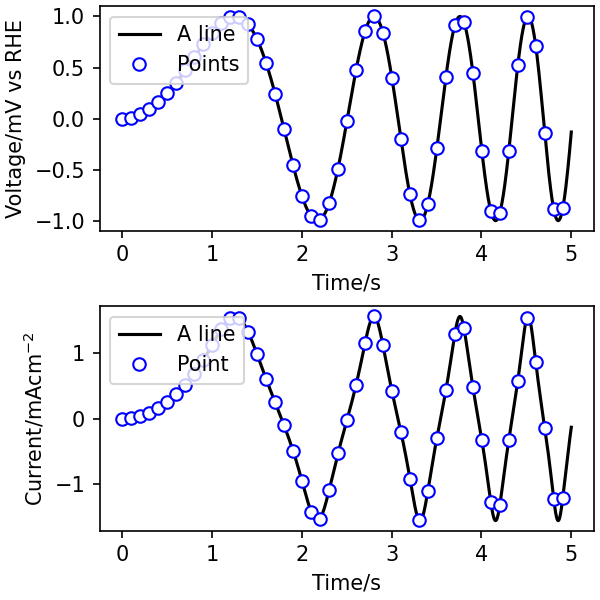
\includegraphics[width=\linewidth]{./figs/png/example_1}
        \caption{.png}
        \label{figures:fig:exmaple:2:png}
        \end{subfigure}
        \hfill
        \begin{subfigure}[t]{0.45\textwidth}
        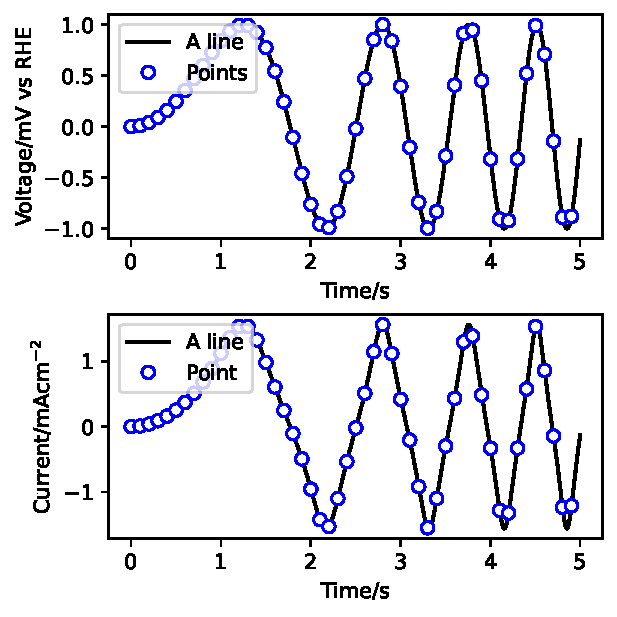
\includegraphics[width=\linewidth]{./figs/pdf/example_1}
        \caption{.pdf}
        \label{figures:fig:exmaple:2:pdf}
        \end{subfigure}
        %
        \begin{subfigure}[t]{0.45\textwidth}
        \resizebox*{\linewidth}{!}{%% Creator: Matplotlib, PGF backend
%%
%% To include the figure in your LaTeX document, write
%%   \input{<filename>.pgf}
%%
%% Make sure the required packages are loaded in your preamble
%%   \usepackage{pgf}
%%
%% Also ensure that all the required font packages are loaded; for instance,
%% the lmodern package is sometimes necessary when using math font.
%%   \usepackage{lmodern}
%%
%% Figures using additional raster images can only be included by \input if
%% they are in the same directory as the main LaTeX file. For loading figures
%% from other directories you can use the `import` package
%%   \usepackage{import}
%%
%% and then include the figures with
%%   \import{<path to file>}{<filename>.pgf}
%%
%% Matplotlib used the following preamble
%%   \usepackage{fontspec}
%%   \setmainfont{DejaVuSerif.ttf}[Path=\detokenize{C:/Users/kristian/anaconda3/lib/site-packages/matplotlib/mpl-data/fonts/ttf/}]
%%   \setsansfont{DejaVuSans.ttf}[Path=\detokenize{C:/Users/kristian/anaconda3/lib/site-packages/matplotlib/mpl-data/fonts/ttf/}]
%%   \setmonofont{DejaVuSansMono.ttf}[Path=\detokenize{C:/Users/kristian/anaconda3/lib/site-packages/matplotlib/mpl-data/fonts/ttf/}]
%%
\begingroup%
\makeatletter%
\begin{pgfpicture}%
\pgfpathrectangle{\pgfpointorigin}{\pgfqpoint{4.000000in}{4.000000in}}%
\pgfusepath{use as bounding box, clip}%
\begin{pgfscope}%
\pgfsetbuttcap%
\pgfsetmiterjoin%
\definecolor{currentfill}{rgb}{1.000000,1.000000,1.000000}%
\pgfsetfillcolor{currentfill}%
\pgfsetlinewidth{0.000000pt}%
\definecolor{currentstroke}{rgb}{1.000000,1.000000,1.000000}%
\pgfsetstrokecolor{currentstroke}%
\pgfsetdash{}{0pt}%
\pgfpathmoveto{\pgfqpoint{0.000000in}{0.000000in}}%
\pgfpathlineto{\pgfqpoint{4.000000in}{0.000000in}}%
\pgfpathlineto{\pgfqpoint{4.000000in}{4.000000in}}%
\pgfpathlineto{\pgfqpoint{0.000000in}{4.000000in}}%
\pgfpathlineto{\pgfqpoint{0.000000in}{0.000000in}}%
\pgfpathclose%
\pgfusepath{fill}%
\end{pgfscope}%
\begin{pgfscope}%
\pgfsetbuttcap%
\pgfsetmiterjoin%
\definecolor{currentfill}{rgb}{1.000000,1.000000,1.000000}%
\pgfsetfillcolor{currentfill}%
\pgfsetlinewidth{0.000000pt}%
\definecolor{currentstroke}{rgb}{0.000000,0.000000,0.000000}%
\pgfsetstrokecolor{currentstroke}%
\pgfsetstrokeopacity{0.000000}%
\pgfsetdash{}{0pt}%
\pgfpathmoveto{\pgfqpoint{0.657765in}{2.463273in}}%
\pgfpathlineto{\pgfqpoint{3.958330in}{2.463273in}}%
\pgfpathlineto{\pgfqpoint{3.958330in}{3.958330in}}%
\pgfpathlineto{\pgfqpoint{0.657765in}{3.958330in}}%
\pgfpathlineto{\pgfqpoint{0.657765in}{2.463273in}}%
\pgfpathclose%
\pgfusepath{fill}%
\end{pgfscope}%
\begin{pgfscope}%
\pgfsetbuttcap%
\pgfsetroundjoin%
\definecolor{currentfill}{rgb}{0.000000,0.000000,0.000000}%
\pgfsetfillcolor{currentfill}%
\pgfsetlinewidth{0.803000pt}%
\definecolor{currentstroke}{rgb}{0.000000,0.000000,0.000000}%
\pgfsetstrokecolor{currentstroke}%
\pgfsetdash{}{0pt}%
\pgfsys@defobject{currentmarker}{\pgfqpoint{0.000000in}{-0.048611in}}{\pgfqpoint{0.000000in}{0.000000in}}{%
\pgfpathmoveto{\pgfqpoint{0.000000in}{0.000000in}}%
\pgfpathlineto{\pgfqpoint{0.000000in}{-0.048611in}}%
\pgfusepath{stroke,fill}%
}%
\begin{pgfscope}%
\pgfsys@transformshift{0.807791in}{2.463273in}%
\pgfsys@useobject{currentmarker}{}%
\end{pgfscope}%
\end{pgfscope}%
\begin{pgfscope}%
\definecolor{textcolor}{rgb}{0.000000,0.000000,0.000000}%
\pgfsetstrokecolor{textcolor}%
\pgfsetfillcolor{textcolor}%
\pgftext[x=0.807791in,y=2.366051in,,top]{\color{textcolor}\sffamily\fontsize{10.000000}{12.000000}\selectfont 0}%
\end{pgfscope}%
\begin{pgfscope}%
\pgfsetbuttcap%
\pgfsetroundjoin%
\definecolor{currentfill}{rgb}{0.000000,0.000000,0.000000}%
\pgfsetfillcolor{currentfill}%
\pgfsetlinewidth{0.803000pt}%
\definecolor{currentstroke}{rgb}{0.000000,0.000000,0.000000}%
\pgfsetstrokecolor{currentstroke}%
\pgfsetdash{}{0pt}%
\pgfsys@defobject{currentmarker}{\pgfqpoint{0.000000in}{-0.048611in}}{\pgfqpoint{0.000000in}{0.000000in}}{%
\pgfpathmoveto{\pgfqpoint{0.000000in}{0.000000in}}%
\pgfpathlineto{\pgfqpoint{0.000000in}{-0.048611in}}%
\pgfusepath{stroke,fill}%
}%
\begin{pgfscope}%
\pgfsys@transformshift{1.407893in}{2.463273in}%
\pgfsys@useobject{currentmarker}{}%
\end{pgfscope}%
\end{pgfscope}%
\begin{pgfscope}%
\definecolor{textcolor}{rgb}{0.000000,0.000000,0.000000}%
\pgfsetstrokecolor{textcolor}%
\pgfsetfillcolor{textcolor}%
\pgftext[x=1.407893in,y=2.366051in,,top]{\color{textcolor}\sffamily\fontsize{10.000000}{12.000000}\selectfont 1}%
\end{pgfscope}%
\begin{pgfscope}%
\pgfsetbuttcap%
\pgfsetroundjoin%
\definecolor{currentfill}{rgb}{0.000000,0.000000,0.000000}%
\pgfsetfillcolor{currentfill}%
\pgfsetlinewidth{0.803000pt}%
\definecolor{currentstroke}{rgb}{0.000000,0.000000,0.000000}%
\pgfsetstrokecolor{currentstroke}%
\pgfsetdash{}{0pt}%
\pgfsys@defobject{currentmarker}{\pgfqpoint{0.000000in}{-0.048611in}}{\pgfqpoint{0.000000in}{0.000000in}}{%
\pgfpathmoveto{\pgfqpoint{0.000000in}{0.000000in}}%
\pgfpathlineto{\pgfqpoint{0.000000in}{-0.048611in}}%
\pgfusepath{stroke,fill}%
}%
\begin{pgfscope}%
\pgfsys@transformshift{2.007996in}{2.463273in}%
\pgfsys@useobject{currentmarker}{}%
\end{pgfscope}%
\end{pgfscope}%
\begin{pgfscope}%
\definecolor{textcolor}{rgb}{0.000000,0.000000,0.000000}%
\pgfsetstrokecolor{textcolor}%
\pgfsetfillcolor{textcolor}%
\pgftext[x=2.007996in,y=2.366051in,,top]{\color{textcolor}\sffamily\fontsize{10.000000}{12.000000}\selectfont 2}%
\end{pgfscope}%
\begin{pgfscope}%
\pgfsetbuttcap%
\pgfsetroundjoin%
\definecolor{currentfill}{rgb}{0.000000,0.000000,0.000000}%
\pgfsetfillcolor{currentfill}%
\pgfsetlinewidth{0.803000pt}%
\definecolor{currentstroke}{rgb}{0.000000,0.000000,0.000000}%
\pgfsetstrokecolor{currentstroke}%
\pgfsetdash{}{0pt}%
\pgfsys@defobject{currentmarker}{\pgfqpoint{0.000000in}{-0.048611in}}{\pgfqpoint{0.000000in}{0.000000in}}{%
\pgfpathmoveto{\pgfqpoint{0.000000in}{0.000000in}}%
\pgfpathlineto{\pgfqpoint{0.000000in}{-0.048611in}}%
\pgfusepath{stroke,fill}%
}%
\begin{pgfscope}%
\pgfsys@transformshift{2.608099in}{2.463273in}%
\pgfsys@useobject{currentmarker}{}%
\end{pgfscope}%
\end{pgfscope}%
\begin{pgfscope}%
\definecolor{textcolor}{rgb}{0.000000,0.000000,0.000000}%
\pgfsetstrokecolor{textcolor}%
\pgfsetfillcolor{textcolor}%
\pgftext[x=2.608099in,y=2.366051in,,top]{\color{textcolor}\sffamily\fontsize{10.000000}{12.000000}\selectfont 3}%
\end{pgfscope}%
\begin{pgfscope}%
\pgfsetbuttcap%
\pgfsetroundjoin%
\definecolor{currentfill}{rgb}{0.000000,0.000000,0.000000}%
\pgfsetfillcolor{currentfill}%
\pgfsetlinewidth{0.803000pt}%
\definecolor{currentstroke}{rgb}{0.000000,0.000000,0.000000}%
\pgfsetstrokecolor{currentstroke}%
\pgfsetdash{}{0pt}%
\pgfsys@defobject{currentmarker}{\pgfqpoint{0.000000in}{-0.048611in}}{\pgfqpoint{0.000000in}{0.000000in}}{%
\pgfpathmoveto{\pgfqpoint{0.000000in}{0.000000in}}%
\pgfpathlineto{\pgfqpoint{0.000000in}{-0.048611in}}%
\pgfusepath{stroke,fill}%
}%
\begin{pgfscope}%
\pgfsys@transformshift{3.208202in}{2.463273in}%
\pgfsys@useobject{currentmarker}{}%
\end{pgfscope}%
\end{pgfscope}%
\begin{pgfscope}%
\definecolor{textcolor}{rgb}{0.000000,0.000000,0.000000}%
\pgfsetstrokecolor{textcolor}%
\pgfsetfillcolor{textcolor}%
\pgftext[x=3.208202in,y=2.366051in,,top]{\color{textcolor}\sffamily\fontsize{10.000000}{12.000000}\selectfont 4}%
\end{pgfscope}%
\begin{pgfscope}%
\pgfsetbuttcap%
\pgfsetroundjoin%
\definecolor{currentfill}{rgb}{0.000000,0.000000,0.000000}%
\pgfsetfillcolor{currentfill}%
\pgfsetlinewidth{0.803000pt}%
\definecolor{currentstroke}{rgb}{0.000000,0.000000,0.000000}%
\pgfsetstrokecolor{currentstroke}%
\pgfsetdash{}{0pt}%
\pgfsys@defobject{currentmarker}{\pgfqpoint{0.000000in}{-0.048611in}}{\pgfqpoint{0.000000in}{0.000000in}}{%
\pgfpathmoveto{\pgfqpoint{0.000000in}{0.000000in}}%
\pgfpathlineto{\pgfqpoint{0.000000in}{-0.048611in}}%
\pgfusepath{stroke,fill}%
}%
\begin{pgfscope}%
\pgfsys@transformshift{3.808304in}{2.463273in}%
\pgfsys@useobject{currentmarker}{}%
\end{pgfscope}%
\end{pgfscope}%
\begin{pgfscope}%
\definecolor{textcolor}{rgb}{0.000000,0.000000,0.000000}%
\pgfsetstrokecolor{textcolor}%
\pgfsetfillcolor{textcolor}%
\pgftext[x=3.808304in,y=2.366051in,,top]{\color{textcolor}\sffamily\fontsize{10.000000}{12.000000}\selectfont 5}%
\end{pgfscope}%
\begin{pgfscope}%
\definecolor{textcolor}{rgb}{0.000000,0.000000,0.000000}%
\pgfsetstrokecolor{textcolor}%
\pgfsetfillcolor{textcolor}%
\pgftext[x=2.308048in,y=2.176083in,,top]{\color{textcolor}\sffamily\fontsize{10.000000}{12.000000}\selectfont Time/s}%
\end{pgfscope}%
\begin{pgfscope}%
\pgfsetbuttcap%
\pgfsetroundjoin%
\definecolor{currentfill}{rgb}{0.000000,0.000000,0.000000}%
\pgfsetfillcolor{currentfill}%
\pgfsetlinewidth{0.803000pt}%
\definecolor{currentstroke}{rgb}{0.000000,0.000000,0.000000}%
\pgfsetstrokecolor{currentstroke}%
\pgfsetdash{}{0pt}%
\pgfsys@defobject{currentmarker}{\pgfqpoint{-0.048611in}{0.000000in}}{\pgfqpoint{-0.000000in}{0.000000in}}{%
\pgfpathmoveto{\pgfqpoint{-0.000000in}{0.000000in}}%
\pgfpathlineto{\pgfqpoint{-0.048611in}{0.000000in}}%
\pgfusepath{stroke,fill}%
}%
\begin{pgfscope}%
\pgfsys@transformshift{0.657765in}{2.531218in}%
\pgfsys@useobject{currentmarker}{}%
\end{pgfscope}%
\end{pgfscope}%
\begin{pgfscope}%
\definecolor{textcolor}{rgb}{0.000000,0.000000,0.000000}%
\pgfsetstrokecolor{textcolor}%
\pgfsetfillcolor{textcolor}%
\pgftext[x=0.231638in, y=2.478457in, left, base]{\color{textcolor}\sffamily\fontsize{10.000000}{12.000000}\selectfont \ensuremath{-}1.0}%
\end{pgfscope}%
\begin{pgfscope}%
\pgfsetbuttcap%
\pgfsetroundjoin%
\definecolor{currentfill}{rgb}{0.000000,0.000000,0.000000}%
\pgfsetfillcolor{currentfill}%
\pgfsetlinewidth{0.803000pt}%
\definecolor{currentstroke}{rgb}{0.000000,0.000000,0.000000}%
\pgfsetstrokecolor{currentstroke}%
\pgfsetdash{}{0pt}%
\pgfsys@defobject{currentmarker}{\pgfqpoint{-0.048611in}{0.000000in}}{\pgfqpoint{-0.000000in}{0.000000in}}{%
\pgfpathmoveto{\pgfqpoint{-0.000000in}{0.000000in}}%
\pgfpathlineto{\pgfqpoint{-0.048611in}{0.000000in}}%
\pgfusepath{stroke,fill}%
}%
\begin{pgfscope}%
\pgfsys@transformshift{0.657765in}{2.871007in}%
\pgfsys@useobject{currentmarker}{}%
\end{pgfscope}%
\end{pgfscope}%
\begin{pgfscope}%
\definecolor{textcolor}{rgb}{0.000000,0.000000,0.000000}%
\pgfsetstrokecolor{textcolor}%
\pgfsetfillcolor{textcolor}%
\pgftext[x=0.231638in, y=2.818246in, left, base]{\color{textcolor}\sffamily\fontsize{10.000000}{12.000000}\selectfont \ensuremath{-}0.5}%
\end{pgfscope}%
\begin{pgfscope}%
\pgfsetbuttcap%
\pgfsetroundjoin%
\definecolor{currentfill}{rgb}{0.000000,0.000000,0.000000}%
\pgfsetfillcolor{currentfill}%
\pgfsetlinewidth{0.803000pt}%
\definecolor{currentstroke}{rgb}{0.000000,0.000000,0.000000}%
\pgfsetstrokecolor{currentstroke}%
\pgfsetdash{}{0pt}%
\pgfsys@defobject{currentmarker}{\pgfqpoint{-0.048611in}{0.000000in}}{\pgfqpoint{-0.000000in}{0.000000in}}{%
\pgfpathmoveto{\pgfqpoint{-0.000000in}{0.000000in}}%
\pgfpathlineto{\pgfqpoint{-0.048611in}{0.000000in}}%
\pgfusepath{stroke,fill}%
}%
\begin{pgfscope}%
\pgfsys@transformshift{0.657765in}{3.210796in}%
\pgfsys@useobject{currentmarker}{}%
\end{pgfscope}%
\end{pgfscope}%
\begin{pgfscope}%
\definecolor{textcolor}{rgb}{0.000000,0.000000,0.000000}%
\pgfsetstrokecolor{textcolor}%
\pgfsetfillcolor{textcolor}%
\pgftext[x=0.339663in, y=3.158035in, left, base]{\color{textcolor}\sffamily\fontsize{10.000000}{12.000000}\selectfont 0.0}%
\end{pgfscope}%
\begin{pgfscope}%
\pgfsetbuttcap%
\pgfsetroundjoin%
\definecolor{currentfill}{rgb}{0.000000,0.000000,0.000000}%
\pgfsetfillcolor{currentfill}%
\pgfsetlinewidth{0.803000pt}%
\definecolor{currentstroke}{rgb}{0.000000,0.000000,0.000000}%
\pgfsetstrokecolor{currentstroke}%
\pgfsetdash{}{0pt}%
\pgfsys@defobject{currentmarker}{\pgfqpoint{-0.048611in}{0.000000in}}{\pgfqpoint{-0.000000in}{0.000000in}}{%
\pgfpathmoveto{\pgfqpoint{-0.000000in}{0.000000in}}%
\pgfpathlineto{\pgfqpoint{-0.048611in}{0.000000in}}%
\pgfusepath{stroke,fill}%
}%
\begin{pgfscope}%
\pgfsys@transformshift{0.657765in}{3.550585in}%
\pgfsys@useobject{currentmarker}{}%
\end{pgfscope}%
\end{pgfscope}%
\begin{pgfscope}%
\definecolor{textcolor}{rgb}{0.000000,0.000000,0.000000}%
\pgfsetstrokecolor{textcolor}%
\pgfsetfillcolor{textcolor}%
\pgftext[x=0.339663in, y=3.497824in, left, base]{\color{textcolor}\sffamily\fontsize{10.000000}{12.000000}\selectfont 0.5}%
\end{pgfscope}%
\begin{pgfscope}%
\pgfsetbuttcap%
\pgfsetroundjoin%
\definecolor{currentfill}{rgb}{0.000000,0.000000,0.000000}%
\pgfsetfillcolor{currentfill}%
\pgfsetlinewidth{0.803000pt}%
\definecolor{currentstroke}{rgb}{0.000000,0.000000,0.000000}%
\pgfsetstrokecolor{currentstroke}%
\pgfsetdash{}{0pt}%
\pgfsys@defobject{currentmarker}{\pgfqpoint{-0.048611in}{0.000000in}}{\pgfqpoint{-0.000000in}{0.000000in}}{%
\pgfpathmoveto{\pgfqpoint{-0.000000in}{0.000000in}}%
\pgfpathlineto{\pgfqpoint{-0.048611in}{0.000000in}}%
\pgfusepath{stroke,fill}%
}%
\begin{pgfscope}%
\pgfsys@transformshift{0.657765in}{3.890374in}%
\pgfsys@useobject{currentmarker}{}%
\end{pgfscope}%
\end{pgfscope}%
\begin{pgfscope}%
\definecolor{textcolor}{rgb}{0.000000,0.000000,0.000000}%
\pgfsetstrokecolor{textcolor}%
\pgfsetfillcolor{textcolor}%
\pgftext[x=0.339663in, y=3.837612in, left, base]{\color{textcolor}\sffamily\fontsize{10.000000}{12.000000}\selectfont 1.0}%
\end{pgfscope}%
\begin{pgfscope}%
\definecolor{textcolor}{rgb}{0.000000,0.000000,0.000000}%
\pgfsetstrokecolor{textcolor}%
\pgfsetfillcolor{textcolor}%
\pgftext[x=0.176083in,y=3.210802in,,bottom,rotate=90.000000]{\color{textcolor}\sffamily\fontsize{10.000000}{12.000000}\selectfont Voltage/mV vs RHE}%
\end{pgfscope}%
\begin{pgfscope}%
\pgfpathrectangle{\pgfqpoint{0.657765in}{2.463273in}}{\pgfqpoint{3.300565in}{1.495057in}}%
\pgfusepath{clip}%
\pgfsetrectcap%
\pgfsetroundjoin%
\pgfsetlinewidth{1.505625pt}%
\definecolor{currentstroke}{rgb}{0.000000,0.000000,0.000000}%
\pgfsetstrokecolor{currentstroke}%
\pgfsetdash{}{0pt}%
\pgfpathmoveto{\pgfqpoint{0.807791in}{3.210796in}}%
\pgfpathlineto{\pgfqpoint{0.831819in}{3.211886in}}%
\pgfpathlineto{\pgfqpoint{0.855847in}{3.215154in}}%
\pgfpathlineto{\pgfqpoint{0.879875in}{3.220601in}}%
\pgfpathlineto{\pgfqpoint{0.903903in}{3.228226in}}%
\pgfpathlineto{\pgfqpoint{0.927931in}{3.238026in}}%
\pgfpathlineto{\pgfqpoint{0.954963in}{3.251645in}}%
\pgfpathlineto{\pgfqpoint{0.981995in}{3.267995in}}%
\pgfpathlineto{\pgfqpoint{1.009026in}{3.287054in}}%
\pgfpathlineto{\pgfqpoint{1.036058in}{3.308781in}}%
\pgfpathlineto{\pgfqpoint{1.066093in}{3.335983in}}%
\pgfpathlineto{\pgfqpoint{1.096128in}{3.366295in}}%
\pgfpathlineto{\pgfqpoint{1.129167in}{3.403037in}}%
\pgfpathlineto{\pgfqpoint{1.162206in}{3.443054in}}%
\pgfpathlineto{\pgfqpoint{1.201251in}{3.494021in}}%
\pgfpathlineto{\pgfqpoint{1.246304in}{3.556669in}}%
\pgfpathlineto{\pgfqpoint{1.390473in}{3.760709in}}%
\pgfpathlineto{\pgfqpoint{1.420508in}{3.797720in}}%
\pgfpathlineto{\pgfqpoint{1.444536in}{3.824206in}}%
\pgfpathlineto{\pgfqpoint{1.465561in}{3.844540in}}%
\pgfpathlineto{\pgfqpoint{1.486586in}{3.861737in}}%
\pgfpathlineto{\pgfqpoint{1.504607in}{3.873621in}}%
\pgfpathlineto{\pgfqpoint{1.519624in}{3.881282in}}%
\pgfpathlineto{\pgfqpoint{1.534642in}{3.886719in}}%
\pgfpathlineto{\pgfqpoint{1.549659in}{3.889760in}}%
\pgfpathlineto{\pgfqpoint{1.564677in}{3.890238in}}%
\pgfpathlineto{\pgfqpoint{1.576691in}{3.888667in}}%
\pgfpathlineto{\pgfqpoint{1.588705in}{3.885274in}}%
\pgfpathlineto{\pgfqpoint{1.600719in}{3.879983in}}%
\pgfpathlineto{\pgfqpoint{1.615737in}{3.870595in}}%
\pgfpathlineto{\pgfqpoint{1.630754in}{3.858009in}}%
\pgfpathlineto{\pgfqpoint{1.645772in}{3.842116in}}%
\pgfpathlineto{\pgfqpoint{1.660790in}{3.822826in}}%
\pgfpathlineto{\pgfqpoint{1.675807in}{3.800070in}}%
\pgfpathlineto{\pgfqpoint{1.693828in}{3.768127in}}%
\pgfpathlineto{\pgfqpoint{1.711849in}{3.731106in}}%
\pgfpathlineto{\pgfqpoint{1.729870in}{3.689042in}}%
\pgfpathlineto{\pgfqpoint{1.750895in}{3.633739in}}%
\pgfpathlineto{\pgfqpoint{1.771920in}{3.572013in}}%
\pgfpathlineto{\pgfqpoint{1.795948in}{3.494183in}}%
\pgfpathlineto{\pgfqpoint{1.822979in}{3.398452in}}%
\pgfpathlineto{\pgfqpoint{1.856018in}{3.272193in}}%
\pgfpathlineto{\pgfqpoint{1.910081in}{3.054295in}}%
\pgfpathlineto{\pgfqpoint{1.952131in}{2.888154in}}%
\pgfpathlineto{\pgfqpoint{1.979162in}{2.789575in}}%
\pgfpathlineto{\pgfqpoint{2.000187in}{2.720218in}}%
\pgfpathlineto{\pgfqpoint{2.018208in}{2.667350in}}%
\pgfpathlineto{\pgfqpoint{2.036229in}{2.621718in}}%
\pgfpathlineto{\pgfqpoint{2.051247in}{2.589979in}}%
\pgfpathlineto{\pgfqpoint{2.063261in}{2.569117in}}%
\pgfpathlineto{\pgfqpoint{2.075275in}{2.552576in}}%
\pgfpathlineto{\pgfqpoint{2.084285in}{2.543157in}}%
\pgfpathlineto{\pgfqpoint{2.093296in}{2.536404in}}%
\pgfpathlineto{\pgfqpoint{2.102307in}{2.532403in}}%
\pgfpathlineto{\pgfqpoint{2.111317in}{2.531230in}}%
\pgfpathlineto{\pgfqpoint{2.120328in}{2.532950in}}%
\pgfpathlineto{\pgfqpoint{2.129338in}{2.537614in}}%
\pgfpathlineto{\pgfqpoint{2.138349in}{2.545264in}}%
\pgfpathlineto{\pgfqpoint{2.147359in}{2.555925in}}%
\pgfpathlineto{\pgfqpoint{2.156370in}{2.569609in}}%
\pgfpathlineto{\pgfqpoint{2.168384in}{2.592550in}}%
\pgfpathlineto{\pgfqpoint{2.180398in}{2.620807in}}%
\pgfpathlineto{\pgfqpoint{2.192412in}{2.654280in}}%
\pgfpathlineto{\pgfqpoint{2.207430in}{2.703209in}}%
\pgfpathlineto{\pgfqpoint{2.222447in}{2.759609in}}%
\pgfpathlineto{\pgfqpoint{2.240468in}{2.836346in}}%
\pgfpathlineto{\pgfqpoint{2.261493in}{2.936763in}}%
\pgfpathlineto{\pgfqpoint{2.285521in}{3.062848in}}%
\pgfpathlineto{\pgfqpoint{2.324567in}{3.282163in}}%
\pgfpathlineto{\pgfqpoint{2.366616in}{3.515126in}}%
\pgfpathlineto{\pgfqpoint{2.390644in}{3.634904in}}%
\pgfpathlineto{\pgfqpoint{2.408665in}{3.713773in}}%
\pgfpathlineto{\pgfqpoint{2.423683in}{3.770373in}}%
\pgfpathlineto{\pgfqpoint{2.435697in}{3.808748in}}%
\pgfpathlineto{\pgfqpoint{2.447711in}{3.840333in}}%
\pgfpathlineto{\pgfqpoint{2.456722in}{3.859241in}}%
\pgfpathlineto{\pgfqpoint{2.465732in}{3.873827in}}%
\pgfpathlineto{\pgfqpoint{2.474743in}{3.883920in}}%
\pgfpathlineto{\pgfqpoint{2.480750in}{3.888078in}}%
\pgfpathlineto{\pgfqpoint{2.486757in}{3.890139in}}%
\pgfpathlineto{\pgfqpoint{2.492764in}{3.890072in}}%
\pgfpathlineto{\pgfqpoint{2.498771in}{3.887856in}}%
\pgfpathlineto{\pgfqpoint{2.504778in}{3.883473in}}%
\pgfpathlineto{\pgfqpoint{2.510785in}{3.876916in}}%
\pgfpathlineto{\pgfqpoint{2.519795in}{3.863001in}}%
\pgfpathlineto{\pgfqpoint{2.528806in}{3.844217in}}%
\pgfpathlineto{\pgfqpoint{2.537817in}{3.820626in}}%
\pgfpathlineto{\pgfqpoint{2.549831in}{3.781881in}}%
\pgfpathlineto{\pgfqpoint{2.561845in}{3.735135in}}%
\pgfpathlineto{\pgfqpoint{2.576862in}{3.666200in}}%
\pgfpathlineto{\pgfqpoint{2.591880in}{3.586744in}}%
\pgfpathlineto{\pgfqpoint{2.609901in}{3.479656in}}%
\pgfpathlineto{\pgfqpoint{2.633929in}{3.322195in}}%
\pgfpathlineto{\pgfqpoint{2.706014in}{2.837903in}}%
\pgfpathlineto{\pgfqpoint{2.724035in}{2.736887in}}%
\pgfpathlineto{\pgfqpoint{2.739052in}{2.665161in}}%
\pgfpathlineto{\pgfqpoint{2.751066in}{2.617495in}}%
\pgfpathlineto{\pgfqpoint{2.763080in}{2.579527in}}%
\pgfpathlineto{\pgfqpoint{2.772091in}{2.557921in}}%
\pgfpathlineto{\pgfqpoint{2.781101in}{2.542533in}}%
\pgfpathlineto{\pgfqpoint{2.787108in}{2.535849in}}%
\pgfpathlineto{\pgfqpoint{2.793116in}{2.532091in}}%
\pgfpathlineto{\pgfqpoint{2.799123in}{2.531302in}}%
\pgfpathlineto{\pgfqpoint{2.805130in}{2.533513in}}%
\pgfpathlineto{\pgfqpoint{2.811137in}{2.538741in}}%
\pgfpathlineto{\pgfqpoint{2.817144in}{2.546990in}}%
\pgfpathlineto{\pgfqpoint{2.823151in}{2.558250in}}%
\pgfpathlineto{\pgfqpoint{2.832161in}{2.580728in}}%
\pgfpathlineto{\pgfqpoint{2.841172in}{2.609781in}}%
\pgfpathlineto{\pgfqpoint{2.853186in}{2.658364in}}%
\pgfpathlineto{\pgfqpoint{2.865200in}{2.717534in}}%
\pgfpathlineto{\pgfqpoint{2.880218in}{2.804939in}}%
\pgfpathlineto{\pgfqpoint{2.898239in}{2.926442in}}%
\pgfpathlineto{\pgfqpoint{2.919263in}{3.084856in}}%
\pgfpathlineto{\pgfqpoint{2.982337in}{3.574238in}}%
\pgfpathlineto{\pgfqpoint{2.997355in}{3.672163in}}%
\pgfpathlineto{\pgfqpoint{3.012372in}{3.755359in}}%
\pgfpathlineto{\pgfqpoint{3.024386in}{3.809192in}}%
\pgfpathlineto{\pgfqpoint{3.033397in}{3.841227in}}%
\pgfpathlineto{\pgfqpoint{3.042407in}{3.865563in}}%
\pgfpathlineto{\pgfqpoint{3.048414in}{3.877309in}}%
\pgfpathlineto{\pgfqpoint{3.054422in}{3.885360in}}%
\pgfpathlineto{\pgfqpoint{3.060429in}{3.889639in}}%
\pgfpathlineto{\pgfqpoint{3.066436in}{3.890093in}}%
\pgfpathlineto{\pgfqpoint{3.072443in}{3.886688in}}%
\pgfpathlineto{\pgfqpoint{3.078450in}{3.879412in}}%
\pgfpathlineto{\pgfqpoint{3.084457in}{3.868278in}}%
\pgfpathlineto{\pgfqpoint{3.090464in}{3.853318in}}%
\pgfpathlineto{\pgfqpoint{3.099474in}{3.823836in}}%
\pgfpathlineto{\pgfqpoint{3.108485in}{3.786169in}}%
\pgfpathlineto{\pgfqpoint{3.120499in}{3.723931in}}%
\pgfpathlineto{\pgfqpoint{3.132513in}{3.649145in}}%
\pgfpathlineto{\pgfqpoint{3.147531in}{3.540503in}}%
\pgfpathlineto{\pgfqpoint{3.165552in}{3.393031in}}%
\pgfpathlineto{\pgfqpoint{3.201594in}{3.073075in}}%
\pgfpathlineto{\pgfqpoint{3.225622in}{2.870117in}}%
\pgfpathlineto{\pgfqpoint{3.240640in}{2.758929in}}%
\pgfpathlineto{\pgfqpoint{3.252654in}{2.682666in}}%
\pgfpathlineto{\pgfqpoint{3.264668in}{2.620087in}}%
\pgfpathlineto{\pgfqpoint{3.273678in}{2.583282in}}%
\pgfpathlineto{\pgfqpoint{3.282689in}{2.555904in}}%
\pgfpathlineto{\pgfqpoint{3.288696in}{2.543154in}}%
\pgfpathlineto{\pgfqpoint{3.294703in}{2.534949in}}%
\pgfpathlineto{\pgfqpoint{3.300710in}{2.531379in}}%
\pgfpathlineto{\pgfqpoint{3.303713in}{2.531352in}}%
\pgfpathlineto{\pgfqpoint{3.309720in}{2.534835in}}%
\pgfpathlineto{\pgfqpoint{3.315728in}{2.543038in}}%
\pgfpathlineto{\pgfqpoint{3.321735in}{2.555938in}}%
\pgfpathlineto{\pgfqpoint{3.327742in}{2.573478in}}%
\pgfpathlineto{\pgfqpoint{3.336752in}{2.608279in}}%
\pgfpathlineto{\pgfqpoint{3.345763in}{2.652857in}}%
\pgfpathlineto{\pgfqpoint{3.357777in}{2.726415in}}%
\pgfpathlineto{\pgfqpoint{3.369791in}{2.814338in}}%
\pgfpathlineto{\pgfqpoint{3.384808in}{2.940788in}}%
\pgfpathlineto{\pgfqpoint{3.405833in}{3.138583in}}%
\pgfpathlineto{\pgfqpoint{3.447882in}{3.539676in}}%
\pgfpathlineto{\pgfqpoint{3.462900in}{3.661944in}}%
\pgfpathlineto{\pgfqpoint{3.474914in}{3.744616in}}%
\pgfpathlineto{\pgfqpoint{3.486928in}{3.810758in}}%
\pgfpathlineto{\pgfqpoint{3.495939in}{3.848091in}}%
\pgfpathlineto{\pgfqpoint{3.501946in}{3.866681in}}%
\pgfpathlineto{\pgfqpoint{3.507953in}{3.880011in}}%
\pgfpathlineto{\pgfqpoint{3.513960in}{3.887939in}}%
\pgfpathlineto{\pgfqpoint{3.516963in}{3.889844in}}%
\pgfpathlineto{\pgfqpoint{3.519967in}{3.890363in}}%
\pgfpathlineto{\pgfqpoint{3.522970in}{3.889491in}}%
\pgfpathlineto{\pgfqpoint{3.525974in}{3.887226in}}%
\pgfpathlineto{\pgfqpoint{3.531981in}{3.878518in}}%
\pgfpathlineto{\pgfqpoint{3.537988in}{3.864273in}}%
\pgfpathlineto{\pgfqpoint{3.543995in}{3.844574in}}%
\pgfpathlineto{\pgfqpoint{3.553005in}{3.805091in}}%
\pgfpathlineto{\pgfqpoint{3.562016in}{3.754263in}}%
\pgfpathlineto{\pgfqpoint{3.574030in}{3.670354in}}%
\pgfpathlineto{\pgfqpoint{3.586044in}{3.570441in}}%
\pgfpathlineto{\pgfqpoint{3.604065in}{3.397765in}}%
\pgfpathlineto{\pgfqpoint{3.664135in}{2.791904in}}%
\pgfpathlineto{\pgfqpoint{3.676150in}{2.697941in}}%
\pgfpathlineto{\pgfqpoint{3.688164in}{2.622356in}}%
\pgfpathlineto{\pgfqpoint{3.697174in}{2.579571in}}%
\pgfpathlineto{\pgfqpoint{3.703181in}{2.558253in}}%
\pgfpathlineto{\pgfqpoint{3.709188in}{2.542980in}}%
\pgfpathlineto{\pgfqpoint{3.715195in}{2.533934in}}%
\pgfpathlineto{\pgfqpoint{3.718199in}{2.531787in}}%
\pgfpathlineto{\pgfqpoint{3.721202in}{2.531238in}}%
\pgfpathlineto{\pgfqpoint{3.724206in}{2.532295in}}%
\pgfpathlineto{\pgfqpoint{3.727209in}{2.534959in}}%
\pgfpathlineto{\pgfqpoint{3.733216in}{2.545099in}}%
\pgfpathlineto{\pgfqpoint{3.739223in}{2.561602in}}%
\pgfpathlineto{\pgfqpoint{3.745230in}{2.584349in}}%
\pgfpathlineto{\pgfqpoint{3.754241in}{2.629766in}}%
\pgfpathlineto{\pgfqpoint{3.763252in}{2.687949in}}%
\pgfpathlineto{\pgfqpoint{3.775266in}{2.783345in}}%
\pgfpathlineto{\pgfqpoint{3.790283in}{2.926179in}}%
\pgfpathlineto{\pgfqpoint{3.808304in}{3.120853in}}%
\pgfpathlineto{\pgfqpoint{3.808304in}{3.120853in}}%
\pgfusepath{stroke}%
\end{pgfscope}%
\begin{pgfscope}%
\pgfpathrectangle{\pgfqpoint{0.657765in}{2.463273in}}{\pgfqpoint{3.300565in}{1.495057in}}%
\pgfusepath{clip}%
\pgfsetbuttcap%
\pgfsetroundjoin%
\definecolor{currentfill}{rgb}{1.000000,1.000000,1.000000}%
\pgfsetfillcolor{currentfill}%
\pgfsetlinewidth{1.003750pt}%
\definecolor{currentstroke}{rgb}{0.000000,0.000000,1.000000}%
\pgfsetstrokecolor{currentstroke}%
\pgfsetdash{}{0pt}%
\pgfsys@defobject{currentmarker}{\pgfqpoint{-0.041667in}{-0.041667in}}{\pgfqpoint{0.041667in}{0.041667in}}{%
\pgfpathmoveto{\pgfqpoint{0.000000in}{-0.041667in}}%
\pgfpathcurveto{\pgfqpoint{0.011050in}{-0.041667in}}{\pgfqpoint{0.021649in}{-0.037276in}}{\pgfqpoint{0.029463in}{-0.029463in}}%
\pgfpathcurveto{\pgfqpoint{0.037276in}{-0.021649in}}{\pgfqpoint{0.041667in}{-0.011050in}}{\pgfqpoint{0.041667in}{0.000000in}}%
\pgfpathcurveto{\pgfqpoint{0.041667in}{0.011050in}}{\pgfqpoint{0.037276in}{0.021649in}}{\pgfqpoint{0.029463in}{0.029463in}}%
\pgfpathcurveto{\pgfqpoint{0.021649in}{0.037276in}}{\pgfqpoint{0.011050in}{0.041667in}}{\pgfqpoint{0.000000in}{0.041667in}}%
\pgfpathcurveto{\pgfqpoint{-0.011050in}{0.041667in}}{\pgfqpoint{-0.021649in}{0.037276in}}{\pgfqpoint{-0.029463in}{0.029463in}}%
\pgfpathcurveto{\pgfqpoint{-0.037276in}{0.021649in}}{\pgfqpoint{-0.041667in}{0.011050in}}{\pgfqpoint{-0.041667in}{0.000000in}}%
\pgfpathcurveto{\pgfqpoint{-0.041667in}{-0.011050in}}{\pgfqpoint{-0.037276in}{-0.021649in}}{\pgfqpoint{-0.029463in}{-0.029463in}}%
\pgfpathcurveto{\pgfqpoint{-0.021649in}{-0.037276in}}{\pgfqpoint{-0.011050in}{-0.041667in}}{\pgfqpoint{0.000000in}{-0.041667in}}%
\pgfpathlineto{\pgfqpoint{0.000000in}{-0.041667in}}%
\pgfpathclose%
\pgfusepath{stroke,fill}%
}%
\begin{pgfscope}%
\pgfsys@transformshift{0.807791in}{3.210796in}%
\pgfsys@useobject{currentmarker}{}%
\end{pgfscope}%
\begin{pgfscope}%
\pgfsys@transformshift{0.867861in}{3.217605in}%
\pgfsys@useobject{currentmarker}{}%
\end{pgfscope}%
\begin{pgfscope}%
\pgfsys@transformshift{0.927931in}{3.238026in}%
\pgfsys@useobject{currentmarker}{}%
\end{pgfscope}%
\begin{pgfscope}%
\pgfsys@transformshift{0.988002in}{3.271998in}%
\pgfsys@useobject{currentmarker}{}%
\end{pgfscope}%
\begin{pgfscope}%
\pgfsys@transformshift{1.048072in}{3.319280in}%
\pgfsys@useobject{currentmarker}{}%
\end{pgfscope}%
\begin{pgfscope}%
\pgfsys@transformshift{1.108142in}{3.379256in}%
\pgfsys@useobject{currentmarker}{}%
\end{pgfscope}%
\begin{pgfscope}%
\pgfsys@transformshift{1.168213in}{3.450652in}%
\pgfsys@useobject{currentmarker}{}%
\end{pgfscope}%
\begin{pgfscope}%
\pgfsys@transformshift{1.228283in}{3.531211in}%
\pgfsys@useobject{currentmarker}{}%
\end{pgfscope}%
\begin{pgfscope}%
\pgfsys@transformshift{1.288353in}{3.617335in}%
\pgfsys@useobject{currentmarker}{}%
\end{pgfscope}%
\begin{pgfscope}%
\pgfsys@transformshift{1.348424in}{3.703765in}%
\pgfsys@useobject{currentmarker}{}%
\end{pgfscope}%
\begin{pgfscope}%
\pgfsys@transformshift{1.408494in}{3.783375in}%
\pgfsys@useobject{currentmarker}{}%
\end{pgfscope}%
\begin{pgfscope}%
\pgfsys@transformshift{1.468564in}{3.847200in}%
\pgfsys@useobject{currentmarker}{}%
\end{pgfscope}%
\begin{pgfscope}%
\pgfsys@transformshift{1.528635in}{3.884822in}%
\pgfsys@useobject{currentmarker}{}%
\end{pgfscope}%
\begin{pgfscope}%
\pgfsys@transformshift{1.588705in}{3.885274in}%
\pgfsys@useobject{currentmarker}{}%
\end{pgfscope}%
\begin{pgfscope}%
\pgfsys@transformshift{1.648775in}{3.838532in}%
\pgfsys@useobject{currentmarker}{}%
\end{pgfscope}%
\begin{pgfscope}%
\pgfsys@transformshift{1.708846in}{3.737628in}%
\pgfsys@useobject{currentmarker}{}%
\end{pgfscope}%
\begin{pgfscope}%
\pgfsys@transformshift{1.768916in}{3.581209in}%
\pgfsys@useobject{currentmarker}{}%
\end{pgfscope}%
\begin{pgfscope}%
\pgfsys@transformshift{1.828987in}{3.376162in}%
\pgfsys@useobject{currentmarker}{}%
\end{pgfscope}%
\begin{pgfscope}%
\pgfsys@transformshift{1.889057in}{3.139641in}%
\pgfsys@useobject{currentmarker}{}%
\end{pgfscope}%
\begin{pgfscope}%
\pgfsys@transformshift{1.949127in}{2.899614in}%
\pgfsys@useobject{currentmarker}{}%
\end{pgfscope}%
\begin{pgfscope}%
\pgfsys@transformshift{2.009198in}{2.692948in}%
\pgfsys@useobject{currentmarker}{}%
\end{pgfscope}%
\begin{pgfscope}%
\pgfsys@transformshift{2.069268in}{2.560290in}%
\pgfsys@useobject{currentmarker}{}%
\end{pgfscope}%
\begin{pgfscope}%
\pgfsys@transformshift{2.129338in}{2.537614in}%
\pgfsys@useobject{currentmarker}{}%
\end{pgfscope}%
\begin{pgfscope}%
\pgfsys@transformshift{2.189409in}{2.645430in}%
\pgfsys@useobject{currentmarker}{}%
\end{pgfscope}%
\begin{pgfscope}%
\pgfsys@transformshift{2.249479in}{2.878065in}%
\pgfsys@useobject{currentmarker}{}%
\end{pgfscope}%
\begin{pgfscope}%
\pgfsys@transformshift{2.309549in}{3.196753in}%
\pgfsys@useobject{currentmarker}{}%
\end{pgfscope}%
\begin{pgfscope}%
\pgfsys@transformshift{2.369620in}{3.530836in}%
\pgfsys@useobject{currentmarker}{}%
\end{pgfscope}%
\begin{pgfscope}%
\pgfsys@transformshift{2.429690in}{3.790373in}%
\pgfsys@useobject{currentmarker}{}%
\end{pgfscope}%
\begin{pgfscope}%
\pgfsys@transformshift{2.489760in}{3.890373in}%
\pgfsys@useobject{currentmarker}{}%
\end{pgfscope}%
\begin{pgfscope}%
\pgfsys@transformshift{2.549831in}{3.781881in}%
\pgfsys@useobject{currentmarker}{}%
\end{pgfscope}%
\begin{pgfscope}%
\pgfsys@transformshift{2.609901in}{3.479656in}%
\pgfsys@useobject{currentmarker}{}%
\end{pgfscope}%
\begin{pgfscope}%
\pgfsys@transformshift{2.669971in}{3.072809in}%
\pgfsys@useobject{currentmarker}{}%
\end{pgfscope}%
\begin{pgfscope}%
\pgfsys@transformshift{2.730042in}{2.706693in}%
\pgfsys@useobject{currentmarker}{}%
\end{pgfscope}%
\begin{pgfscope}%
\pgfsys@transformshift{2.790112in}{2.533601in}%
\pgfsys@useobject{currentmarker}{}%
\end{pgfscope}%
\begin{pgfscope}%
\pgfsys@transformshift{2.850182in}{2.645194in}%
\pgfsys@useobject{currentmarker}{}%
\end{pgfscope}%
\begin{pgfscope}%
\pgfsys@transformshift{2.910253in}{3.015276in}%
\pgfsys@useobject{currentmarker}{}%
\end{pgfscope}%
\begin{pgfscope}%
\pgfsys@transformshift{2.970323in}{3.487646in}%
\pgfsys@useobject{currentmarker}{}%
\end{pgfscope}%
\begin{pgfscope}%
\pgfsys@transformshift{3.030393in}{3.831381in}%
\pgfsys@useobject{currentmarker}{}%
\end{pgfscope}%
\begin{pgfscope}%
\pgfsys@transformshift{3.090464in}{3.853318in}%
\pgfsys@useobject{currentmarker}{}%
\end{pgfscope}%
\begin{pgfscope}%
\pgfsys@transformshift{3.150534in}{3.517050in}%
\pgfsys@useobject{currentmarker}{}%
\end{pgfscope}%
\begin{pgfscope}%
\pgfsys@transformshift{3.210604in}{2.994391in}%
\pgfsys@useobject{currentmarker}{}%
\end{pgfscope}%
\begin{pgfscope}%
\pgfsys@transformshift{3.270675in}{2.594533in}%
\pgfsys@useobject{currentmarker}{}%
\end{pgfscope}%
\begin{pgfscope}%
\pgfsys@transformshift{3.330745in}{2.583961in}%
\pgfsys@useobject{currentmarker}{}%
\end{pgfscope}%
\begin{pgfscope}%
\pgfsys@transformshift{3.390815in}{2.995399in}%
\pgfsys@useobject{currentmarker}{}%
\end{pgfscope}%
\begin{pgfscope}%
\pgfsys@transformshift{3.450886in}{3.565552in}%
\pgfsys@useobject{currentmarker}{}%
\end{pgfscope}%
\begin{pgfscope}%
\pgfsys@transformshift{3.510956in}{3.884658in}%
\pgfsys@useobject{currentmarker}{}%
\end{pgfscope}%
\begin{pgfscope}%
\pgfsys@transformshift{3.571026in}{3.692945in}%
\pgfsys@useobject{currentmarker}{}%
\end{pgfscope}%
\begin{pgfscope}%
\pgfsys@transformshift{3.631097in}{3.113882in}%
\pgfsys@useobject{currentmarker}{}%
\end{pgfscope}%
\begin{pgfscope}%
\pgfsys@transformshift{3.691167in}{2.606700in}%
\pgfsys@useobject{currentmarker}{}%
\end{pgfscope}%
\begin{pgfscope}%
\pgfsys@transformshift{3.751237in}{2.613160in}%
\pgfsys@useobject{currentmarker}{}%
\end{pgfscope}%
\end{pgfscope}%
\begin{pgfscope}%
\pgfsetrectcap%
\pgfsetmiterjoin%
\pgfsetlinewidth{0.803000pt}%
\definecolor{currentstroke}{rgb}{0.000000,0.000000,0.000000}%
\pgfsetstrokecolor{currentstroke}%
\pgfsetdash{}{0pt}%
\pgfpathmoveto{\pgfqpoint{0.657765in}{2.463273in}}%
\pgfpathlineto{\pgfqpoint{0.657765in}{3.958330in}}%
\pgfusepath{stroke}%
\end{pgfscope}%
\begin{pgfscope}%
\pgfsetrectcap%
\pgfsetmiterjoin%
\pgfsetlinewidth{0.803000pt}%
\definecolor{currentstroke}{rgb}{0.000000,0.000000,0.000000}%
\pgfsetstrokecolor{currentstroke}%
\pgfsetdash{}{0pt}%
\pgfpathmoveto{\pgfqpoint{3.958330in}{2.463273in}}%
\pgfpathlineto{\pgfqpoint{3.958330in}{3.958330in}}%
\pgfusepath{stroke}%
\end{pgfscope}%
\begin{pgfscope}%
\pgfsetrectcap%
\pgfsetmiterjoin%
\pgfsetlinewidth{0.803000pt}%
\definecolor{currentstroke}{rgb}{0.000000,0.000000,0.000000}%
\pgfsetstrokecolor{currentstroke}%
\pgfsetdash{}{0pt}%
\pgfpathmoveto{\pgfqpoint{0.657765in}{2.463273in}}%
\pgfpathlineto{\pgfqpoint{3.958330in}{2.463273in}}%
\pgfusepath{stroke}%
\end{pgfscope}%
\begin{pgfscope}%
\pgfsetrectcap%
\pgfsetmiterjoin%
\pgfsetlinewidth{0.803000pt}%
\definecolor{currentstroke}{rgb}{0.000000,0.000000,0.000000}%
\pgfsetstrokecolor{currentstroke}%
\pgfsetdash{}{0pt}%
\pgfpathmoveto{\pgfqpoint{0.657765in}{3.958330in}}%
\pgfpathlineto{\pgfqpoint{3.958330in}{3.958330in}}%
\pgfusepath{stroke}%
\end{pgfscope}%
\begin{pgfscope}%
\pgfsetbuttcap%
\pgfsetmiterjoin%
\definecolor{currentfill}{rgb}{1.000000,1.000000,1.000000}%
\pgfsetfillcolor{currentfill}%
\pgfsetfillopacity{0.800000}%
\pgfsetlinewidth{1.003750pt}%
\definecolor{currentstroke}{rgb}{0.800000,0.800000,0.800000}%
\pgfsetstrokecolor{currentstroke}%
\pgfsetstrokeopacity{0.800000}%
\pgfsetdash{}{0pt}%
\pgfpathmoveto{\pgfqpoint{0.754987in}{3.439504in}}%
\pgfpathlineto{\pgfqpoint{1.616641in}{3.439504in}}%
\pgfpathquadraticcurveto{\pgfqpoint{1.644419in}{3.439504in}}{\pgfqpoint{1.644419in}{3.467282in}}%
\pgfpathlineto{\pgfqpoint{1.644419in}{3.861108in}}%
\pgfpathquadraticcurveto{\pgfqpoint{1.644419in}{3.888886in}}{\pgfqpoint{1.616641in}{3.888886in}}%
\pgfpathlineto{\pgfqpoint{0.754987in}{3.888886in}}%
\pgfpathquadraticcurveto{\pgfqpoint{0.727209in}{3.888886in}}{\pgfqpoint{0.727209in}{3.861108in}}%
\pgfpathlineto{\pgfqpoint{0.727209in}{3.467282in}}%
\pgfpathquadraticcurveto{\pgfqpoint{0.727209in}{3.439504in}}{\pgfqpoint{0.754987in}{3.439504in}}%
\pgfpathlineto{\pgfqpoint{0.754987in}{3.439504in}}%
\pgfpathclose%
\pgfusepath{stroke,fill}%
\end{pgfscope}%
\begin{pgfscope}%
\pgfsetrectcap%
\pgfsetroundjoin%
\pgfsetlinewidth{1.505625pt}%
\definecolor{currentstroke}{rgb}{0.000000,0.000000,0.000000}%
\pgfsetstrokecolor{currentstroke}%
\pgfsetdash{}{0pt}%
\pgfpathmoveto{\pgfqpoint{0.782765in}{3.776418in}}%
\pgfpathlineto{\pgfqpoint{0.921654in}{3.776418in}}%
\pgfpathlineto{\pgfqpoint{1.060543in}{3.776418in}}%
\pgfusepath{stroke}%
\end{pgfscope}%
\begin{pgfscope}%
\definecolor{textcolor}{rgb}{0.000000,0.000000,0.000000}%
\pgfsetstrokecolor{textcolor}%
\pgfsetfillcolor{textcolor}%
\pgftext[x=1.171654in,y=3.727807in,left,base]{\color{textcolor}\sffamily\fontsize{10.000000}{12.000000}\selectfont A line}%
\end{pgfscope}%
\begin{pgfscope}%
\pgfsetbuttcap%
\pgfsetroundjoin%
\definecolor{currentfill}{rgb}{1.000000,1.000000,1.000000}%
\pgfsetfillcolor{currentfill}%
\pgfsetlinewidth{1.003750pt}%
\definecolor{currentstroke}{rgb}{0.000000,0.000000,1.000000}%
\pgfsetstrokecolor{currentstroke}%
\pgfsetdash{}{0pt}%
\pgfsys@defobject{currentmarker}{\pgfqpoint{-0.041667in}{-0.041667in}}{\pgfqpoint{0.041667in}{0.041667in}}{%
\pgfpathmoveto{\pgfqpoint{0.000000in}{-0.041667in}}%
\pgfpathcurveto{\pgfqpoint{0.011050in}{-0.041667in}}{\pgfqpoint{0.021649in}{-0.037276in}}{\pgfqpoint{0.029463in}{-0.029463in}}%
\pgfpathcurveto{\pgfqpoint{0.037276in}{-0.021649in}}{\pgfqpoint{0.041667in}{-0.011050in}}{\pgfqpoint{0.041667in}{0.000000in}}%
\pgfpathcurveto{\pgfqpoint{0.041667in}{0.011050in}}{\pgfqpoint{0.037276in}{0.021649in}}{\pgfqpoint{0.029463in}{0.029463in}}%
\pgfpathcurveto{\pgfqpoint{0.021649in}{0.037276in}}{\pgfqpoint{0.011050in}{0.041667in}}{\pgfqpoint{0.000000in}{0.041667in}}%
\pgfpathcurveto{\pgfqpoint{-0.011050in}{0.041667in}}{\pgfqpoint{-0.021649in}{0.037276in}}{\pgfqpoint{-0.029463in}{0.029463in}}%
\pgfpathcurveto{\pgfqpoint{-0.037276in}{0.021649in}}{\pgfqpoint{-0.041667in}{0.011050in}}{\pgfqpoint{-0.041667in}{0.000000in}}%
\pgfpathcurveto{\pgfqpoint{-0.041667in}{-0.011050in}}{\pgfqpoint{-0.037276in}{-0.021649in}}{\pgfqpoint{-0.029463in}{-0.029463in}}%
\pgfpathcurveto{\pgfqpoint{-0.021649in}{-0.037276in}}{\pgfqpoint{-0.011050in}{-0.041667in}}{\pgfqpoint{0.000000in}{-0.041667in}}%
\pgfpathlineto{\pgfqpoint{0.000000in}{-0.041667in}}%
\pgfpathclose%
\pgfusepath{stroke,fill}%
}%
\begin{pgfscope}%
\pgfsys@transformshift{0.921654in}{3.572561in}%
\pgfsys@useobject{currentmarker}{}%
\end{pgfscope}%
\end{pgfscope}%
\begin{pgfscope}%
\definecolor{textcolor}{rgb}{0.000000,0.000000,0.000000}%
\pgfsetstrokecolor{textcolor}%
\pgfsetfillcolor{textcolor}%
\pgftext[x=1.171654in,y=3.523950in,left,base]{\color{textcolor}\sffamily\fontsize{10.000000}{12.000000}\selectfont Points}%
\end{pgfscope}%
\begin{pgfscope}%
\pgfsetbuttcap%
\pgfsetmiterjoin%
\definecolor{currentfill}{rgb}{1.000000,1.000000,1.000000}%
\pgfsetfillcolor{currentfill}%
\pgfsetlinewidth{0.000000pt}%
\definecolor{currentstroke}{rgb}{0.000000,0.000000,0.000000}%
\pgfsetstrokecolor{currentstroke}%
\pgfsetstrokeopacity{0.000000}%
\pgfsetdash{}{0pt}%
\pgfpathmoveto{\pgfqpoint{0.657765in}{0.463273in}}%
\pgfpathlineto{\pgfqpoint{3.958330in}{0.463273in}}%
\pgfpathlineto{\pgfqpoint{3.958330in}{1.958330in}}%
\pgfpathlineto{\pgfqpoint{0.657765in}{1.958330in}}%
\pgfpathlineto{\pgfqpoint{0.657765in}{0.463273in}}%
\pgfpathclose%
\pgfusepath{fill}%
\end{pgfscope}%
\begin{pgfscope}%
\pgfsetbuttcap%
\pgfsetroundjoin%
\definecolor{currentfill}{rgb}{0.000000,0.000000,0.000000}%
\pgfsetfillcolor{currentfill}%
\pgfsetlinewidth{0.803000pt}%
\definecolor{currentstroke}{rgb}{0.000000,0.000000,0.000000}%
\pgfsetstrokecolor{currentstroke}%
\pgfsetdash{}{0pt}%
\pgfsys@defobject{currentmarker}{\pgfqpoint{0.000000in}{-0.048611in}}{\pgfqpoint{0.000000in}{0.000000in}}{%
\pgfpathmoveto{\pgfqpoint{0.000000in}{0.000000in}}%
\pgfpathlineto{\pgfqpoint{0.000000in}{-0.048611in}}%
\pgfusepath{stroke,fill}%
}%
\begin{pgfscope}%
\pgfsys@transformshift{0.807791in}{0.463273in}%
\pgfsys@useobject{currentmarker}{}%
\end{pgfscope}%
\end{pgfscope}%
\begin{pgfscope}%
\definecolor{textcolor}{rgb}{0.000000,0.000000,0.000000}%
\pgfsetstrokecolor{textcolor}%
\pgfsetfillcolor{textcolor}%
\pgftext[x=0.807791in,y=0.366051in,,top]{\color{textcolor}\sffamily\fontsize{10.000000}{12.000000}\selectfont 0}%
\end{pgfscope}%
\begin{pgfscope}%
\pgfsetbuttcap%
\pgfsetroundjoin%
\definecolor{currentfill}{rgb}{0.000000,0.000000,0.000000}%
\pgfsetfillcolor{currentfill}%
\pgfsetlinewidth{0.803000pt}%
\definecolor{currentstroke}{rgb}{0.000000,0.000000,0.000000}%
\pgfsetstrokecolor{currentstroke}%
\pgfsetdash{}{0pt}%
\pgfsys@defobject{currentmarker}{\pgfqpoint{0.000000in}{-0.048611in}}{\pgfqpoint{0.000000in}{0.000000in}}{%
\pgfpathmoveto{\pgfqpoint{0.000000in}{0.000000in}}%
\pgfpathlineto{\pgfqpoint{0.000000in}{-0.048611in}}%
\pgfusepath{stroke,fill}%
}%
\begin{pgfscope}%
\pgfsys@transformshift{1.407893in}{0.463273in}%
\pgfsys@useobject{currentmarker}{}%
\end{pgfscope}%
\end{pgfscope}%
\begin{pgfscope}%
\definecolor{textcolor}{rgb}{0.000000,0.000000,0.000000}%
\pgfsetstrokecolor{textcolor}%
\pgfsetfillcolor{textcolor}%
\pgftext[x=1.407893in,y=0.366051in,,top]{\color{textcolor}\sffamily\fontsize{10.000000}{12.000000}\selectfont 1}%
\end{pgfscope}%
\begin{pgfscope}%
\pgfsetbuttcap%
\pgfsetroundjoin%
\definecolor{currentfill}{rgb}{0.000000,0.000000,0.000000}%
\pgfsetfillcolor{currentfill}%
\pgfsetlinewidth{0.803000pt}%
\definecolor{currentstroke}{rgb}{0.000000,0.000000,0.000000}%
\pgfsetstrokecolor{currentstroke}%
\pgfsetdash{}{0pt}%
\pgfsys@defobject{currentmarker}{\pgfqpoint{0.000000in}{-0.048611in}}{\pgfqpoint{0.000000in}{0.000000in}}{%
\pgfpathmoveto{\pgfqpoint{0.000000in}{0.000000in}}%
\pgfpathlineto{\pgfqpoint{0.000000in}{-0.048611in}}%
\pgfusepath{stroke,fill}%
}%
\begin{pgfscope}%
\pgfsys@transformshift{2.007996in}{0.463273in}%
\pgfsys@useobject{currentmarker}{}%
\end{pgfscope}%
\end{pgfscope}%
\begin{pgfscope}%
\definecolor{textcolor}{rgb}{0.000000,0.000000,0.000000}%
\pgfsetstrokecolor{textcolor}%
\pgfsetfillcolor{textcolor}%
\pgftext[x=2.007996in,y=0.366051in,,top]{\color{textcolor}\sffamily\fontsize{10.000000}{12.000000}\selectfont 2}%
\end{pgfscope}%
\begin{pgfscope}%
\pgfsetbuttcap%
\pgfsetroundjoin%
\definecolor{currentfill}{rgb}{0.000000,0.000000,0.000000}%
\pgfsetfillcolor{currentfill}%
\pgfsetlinewidth{0.803000pt}%
\definecolor{currentstroke}{rgb}{0.000000,0.000000,0.000000}%
\pgfsetstrokecolor{currentstroke}%
\pgfsetdash{}{0pt}%
\pgfsys@defobject{currentmarker}{\pgfqpoint{0.000000in}{-0.048611in}}{\pgfqpoint{0.000000in}{0.000000in}}{%
\pgfpathmoveto{\pgfqpoint{0.000000in}{0.000000in}}%
\pgfpathlineto{\pgfqpoint{0.000000in}{-0.048611in}}%
\pgfusepath{stroke,fill}%
}%
\begin{pgfscope}%
\pgfsys@transformshift{2.608099in}{0.463273in}%
\pgfsys@useobject{currentmarker}{}%
\end{pgfscope}%
\end{pgfscope}%
\begin{pgfscope}%
\definecolor{textcolor}{rgb}{0.000000,0.000000,0.000000}%
\pgfsetstrokecolor{textcolor}%
\pgfsetfillcolor{textcolor}%
\pgftext[x=2.608099in,y=0.366051in,,top]{\color{textcolor}\sffamily\fontsize{10.000000}{12.000000}\selectfont 3}%
\end{pgfscope}%
\begin{pgfscope}%
\pgfsetbuttcap%
\pgfsetroundjoin%
\definecolor{currentfill}{rgb}{0.000000,0.000000,0.000000}%
\pgfsetfillcolor{currentfill}%
\pgfsetlinewidth{0.803000pt}%
\definecolor{currentstroke}{rgb}{0.000000,0.000000,0.000000}%
\pgfsetstrokecolor{currentstroke}%
\pgfsetdash{}{0pt}%
\pgfsys@defobject{currentmarker}{\pgfqpoint{0.000000in}{-0.048611in}}{\pgfqpoint{0.000000in}{0.000000in}}{%
\pgfpathmoveto{\pgfqpoint{0.000000in}{0.000000in}}%
\pgfpathlineto{\pgfqpoint{0.000000in}{-0.048611in}}%
\pgfusepath{stroke,fill}%
}%
\begin{pgfscope}%
\pgfsys@transformshift{3.208202in}{0.463273in}%
\pgfsys@useobject{currentmarker}{}%
\end{pgfscope}%
\end{pgfscope}%
\begin{pgfscope}%
\definecolor{textcolor}{rgb}{0.000000,0.000000,0.000000}%
\pgfsetstrokecolor{textcolor}%
\pgfsetfillcolor{textcolor}%
\pgftext[x=3.208202in,y=0.366051in,,top]{\color{textcolor}\sffamily\fontsize{10.000000}{12.000000}\selectfont 4}%
\end{pgfscope}%
\begin{pgfscope}%
\pgfsetbuttcap%
\pgfsetroundjoin%
\definecolor{currentfill}{rgb}{0.000000,0.000000,0.000000}%
\pgfsetfillcolor{currentfill}%
\pgfsetlinewidth{0.803000pt}%
\definecolor{currentstroke}{rgb}{0.000000,0.000000,0.000000}%
\pgfsetstrokecolor{currentstroke}%
\pgfsetdash{}{0pt}%
\pgfsys@defobject{currentmarker}{\pgfqpoint{0.000000in}{-0.048611in}}{\pgfqpoint{0.000000in}{0.000000in}}{%
\pgfpathmoveto{\pgfqpoint{0.000000in}{0.000000in}}%
\pgfpathlineto{\pgfqpoint{0.000000in}{-0.048611in}}%
\pgfusepath{stroke,fill}%
}%
\begin{pgfscope}%
\pgfsys@transformshift{3.808304in}{0.463273in}%
\pgfsys@useobject{currentmarker}{}%
\end{pgfscope}%
\end{pgfscope}%
\begin{pgfscope}%
\definecolor{textcolor}{rgb}{0.000000,0.000000,0.000000}%
\pgfsetstrokecolor{textcolor}%
\pgfsetfillcolor{textcolor}%
\pgftext[x=3.808304in,y=0.366051in,,top]{\color{textcolor}\sffamily\fontsize{10.000000}{12.000000}\selectfont 5}%
\end{pgfscope}%
\begin{pgfscope}%
\definecolor{textcolor}{rgb}{0.000000,0.000000,0.000000}%
\pgfsetstrokecolor{textcolor}%
\pgfsetfillcolor{textcolor}%
\pgftext[x=2.308048in,y=0.176083in,,top]{\color{textcolor}\sffamily\fontsize{10.000000}{12.000000}\selectfont Time/s}%
\end{pgfscope}%
\begin{pgfscope}%
\pgfsetbuttcap%
\pgfsetroundjoin%
\definecolor{currentfill}{rgb}{0.000000,0.000000,0.000000}%
\pgfsetfillcolor{currentfill}%
\pgfsetlinewidth{0.803000pt}%
\definecolor{currentstroke}{rgb}{0.000000,0.000000,0.000000}%
\pgfsetstrokecolor{currentstroke}%
\pgfsetdash{}{0pt}%
\pgfsys@defobject{currentmarker}{\pgfqpoint{-0.048611in}{0.000000in}}{\pgfqpoint{-0.000000in}{0.000000in}}{%
\pgfpathmoveto{\pgfqpoint{-0.000000in}{0.000000in}}%
\pgfpathlineto{\pgfqpoint{-0.048611in}{0.000000in}}%
\pgfusepath{stroke,fill}%
}%
\begin{pgfscope}%
\pgfsys@transformshift{0.657765in}{0.774433in}%
\pgfsys@useobject{currentmarker}{}%
\end{pgfscope}%
\end{pgfscope}%
\begin{pgfscope}%
\definecolor{textcolor}{rgb}{0.000000,0.000000,0.000000}%
\pgfsetstrokecolor{textcolor}%
\pgfsetfillcolor{textcolor}%
\pgftext[x=0.364152in, y=0.721671in, left, base]{\color{textcolor}\sffamily\fontsize{10.000000}{12.000000}\selectfont \ensuremath{-}1}%
\end{pgfscope}%
\begin{pgfscope}%
\pgfsetbuttcap%
\pgfsetroundjoin%
\definecolor{currentfill}{rgb}{0.000000,0.000000,0.000000}%
\pgfsetfillcolor{currentfill}%
\pgfsetlinewidth{0.803000pt}%
\definecolor{currentstroke}{rgb}{0.000000,0.000000,0.000000}%
\pgfsetstrokecolor{currentstroke}%
\pgfsetdash{}{0pt}%
\pgfsys@defobject{currentmarker}{\pgfqpoint{-0.048611in}{0.000000in}}{\pgfqpoint{-0.000000in}{0.000000in}}{%
\pgfpathmoveto{\pgfqpoint{-0.000000in}{0.000000in}}%
\pgfpathlineto{\pgfqpoint{-0.048611in}{0.000000in}}%
\pgfusepath{stroke,fill}%
}%
\begin{pgfscope}%
\pgfsys@transformshift{0.657765in}{1.210790in}%
\pgfsys@useobject{currentmarker}{}%
\end{pgfscope}%
\end{pgfscope}%
\begin{pgfscope}%
\definecolor{textcolor}{rgb}{0.000000,0.000000,0.000000}%
\pgfsetstrokecolor{textcolor}%
\pgfsetfillcolor{textcolor}%
\pgftext[x=0.472177in, y=1.158028in, left, base]{\color{textcolor}\sffamily\fontsize{10.000000}{12.000000}\selectfont 0}%
\end{pgfscope}%
\begin{pgfscope}%
\pgfsetbuttcap%
\pgfsetroundjoin%
\definecolor{currentfill}{rgb}{0.000000,0.000000,0.000000}%
\pgfsetfillcolor{currentfill}%
\pgfsetlinewidth{0.803000pt}%
\definecolor{currentstroke}{rgb}{0.000000,0.000000,0.000000}%
\pgfsetstrokecolor{currentstroke}%
\pgfsetdash{}{0pt}%
\pgfsys@defobject{currentmarker}{\pgfqpoint{-0.048611in}{0.000000in}}{\pgfqpoint{-0.000000in}{0.000000in}}{%
\pgfpathmoveto{\pgfqpoint{-0.000000in}{0.000000in}}%
\pgfpathlineto{\pgfqpoint{-0.048611in}{0.000000in}}%
\pgfusepath{stroke,fill}%
}%
\begin{pgfscope}%
\pgfsys@transformshift{0.657765in}{1.647146in}%
\pgfsys@useobject{currentmarker}{}%
\end{pgfscope}%
\end{pgfscope}%
\begin{pgfscope}%
\definecolor{textcolor}{rgb}{0.000000,0.000000,0.000000}%
\pgfsetstrokecolor{textcolor}%
\pgfsetfillcolor{textcolor}%
\pgftext[x=0.472177in, y=1.594385in, left, base]{\color{textcolor}\sffamily\fontsize{10.000000}{12.000000}\selectfont 1}%
\end{pgfscope}%
\begin{pgfscope}%
\definecolor{textcolor}{rgb}{0.000000,0.000000,0.000000}%
\pgfsetstrokecolor{textcolor}%
\pgfsetfillcolor{textcolor}%
\pgftext[x=0.308597in,y=1.210802in,,bottom,rotate=90.000000]{\color{textcolor}\sffamily\fontsize{10.000000}{12.000000}\selectfont Current/mAcm\(\displaystyle ^{-2}\)}%
\end{pgfscope}%
\begin{pgfscope}%
\pgfpathrectangle{\pgfqpoint{0.657765in}{0.463273in}}{\pgfqpoint{3.300565in}{1.495057in}}%
\pgfusepath{clip}%
\pgfsetrectcap%
\pgfsetroundjoin%
\pgfsetlinewidth{1.505625pt}%
\definecolor{currentstroke}{rgb}{0.000000,0.000000,0.000000}%
\pgfsetstrokecolor{currentstroke}%
\pgfsetdash{}{0pt}%
\pgfpathmoveto{\pgfqpoint{0.807791in}{1.210790in}}%
\pgfpathlineto{\pgfqpoint{0.837826in}{1.211883in}}%
\pgfpathlineto{\pgfqpoint{0.867861in}{1.215162in}}%
\pgfpathlineto{\pgfqpoint{0.897896in}{1.220628in}}%
\pgfpathlineto{\pgfqpoint{0.927931in}{1.228283in}}%
\pgfpathlineto{\pgfqpoint{0.957967in}{1.238134in}}%
\pgfpathlineto{\pgfqpoint{0.988002in}{1.250194in}}%
\pgfpathlineto{\pgfqpoint{1.018037in}{1.264485in}}%
\pgfpathlineto{\pgfqpoint{1.048072in}{1.281045in}}%
\pgfpathlineto{\pgfqpoint{1.078107in}{1.299932in}}%
\pgfpathlineto{\pgfqpoint{1.108142in}{1.321229in}}%
\pgfpathlineto{\pgfqpoint{1.138178in}{1.345047in}}%
\pgfpathlineto{\pgfqpoint{1.168213in}{1.371532in}}%
\pgfpathlineto{\pgfqpoint{1.198248in}{1.400866in}}%
\pgfpathlineto{\pgfqpoint{1.228283in}{1.433263in}}%
\pgfpathlineto{\pgfqpoint{1.258318in}{1.468959in}}%
\pgfpathlineto{\pgfqpoint{1.288353in}{1.508181in}}%
\pgfpathlineto{\pgfqpoint{1.318389in}{1.551092in}}%
\pgfpathlineto{\pgfqpoint{1.351427in}{1.602552in}}%
\pgfpathlineto{\pgfqpoint{1.387469in}{1.663204in}}%
\pgfpathlineto{\pgfqpoint{1.477575in}{1.817930in}}%
\pgfpathlineto{\pgfqpoint{1.495596in}{1.843606in}}%
\pgfpathlineto{\pgfqpoint{1.510614in}{1.861709in}}%
\pgfpathlineto{\pgfqpoint{1.522628in}{1.873475in}}%
\pgfpathlineto{\pgfqpoint{1.534642in}{1.882402in}}%
\pgfpathlineto{\pgfqpoint{1.546656in}{1.888131in}}%
\pgfpathlineto{\pgfqpoint{1.555666in}{1.890142in}}%
\pgfpathlineto{\pgfqpoint{1.564677in}{1.890077in}}%
\pgfpathlineto{\pgfqpoint{1.573688in}{1.887861in}}%
\pgfpathlineto{\pgfqpoint{1.582698in}{1.883451in}}%
\pgfpathlineto{\pgfqpoint{1.591709in}{1.876839in}}%
\pgfpathlineto{\pgfqpoint{1.603723in}{1.864647in}}%
\pgfpathlineto{\pgfqpoint{1.615737in}{1.848747in}}%
\pgfpathlineto{\pgfqpoint{1.627751in}{1.829396in}}%
\pgfpathlineto{\pgfqpoint{1.642768in}{1.800875in}}%
\pgfpathlineto{\pgfqpoint{1.660790in}{1.761349in}}%
\pgfpathlineto{\pgfqpoint{1.684818in}{1.702082in}}%
\pgfpathlineto{\pgfqpoint{1.720860in}{1.605723in}}%
\pgfpathlineto{\pgfqpoint{1.795948in}{1.404089in}}%
\pgfpathlineto{\pgfqpoint{1.877043in}{1.196320in}}%
\pgfpathlineto{\pgfqpoint{1.916089in}{1.091897in}}%
\pgfpathlineto{\pgfqpoint{1.946124in}{1.004870in}}%
\pgfpathlineto{\pgfqpoint{1.973155in}{0.919396in}}%
\pgfpathlineto{\pgfqpoint{2.000187in}{0.826616in}}%
\pgfpathlineto{\pgfqpoint{2.057254in}{0.626112in}}%
\pgfpathlineto{\pgfqpoint{2.072271in}{0.583380in}}%
\pgfpathlineto{\pgfqpoint{2.084285in}{0.556766in}}%
\pgfpathlineto{\pgfqpoint{2.093296in}{0.542476in}}%
\pgfpathlineto{\pgfqpoint{2.099303in}{0.536036in}}%
\pgfpathlineto{\pgfqpoint{2.105310in}{0.532251in}}%
\pgfpathlineto{\pgfqpoint{2.111317in}{0.531230in}}%
\pgfpathlineto{\pgfqpoint{2.117324in}{0.533034in}}%
\pgfpathlineto{\pgfqpoint{2.123331in}{0.537664in}}%
\pgfpathlineto{\pgfqpoint{2.129338in}{0.545069in}}%
\pgfpathlineto{\pgfqpoint{2.138349in}{0.561138in}}%
\pgfpathlineto{\pgfqpoint{2.147359in}{0.582655in}}%
\pgfpathlineto{\pgfqpoint{2.159373in}{0.618543in}}%
\pgfpathlineto{\pgfqpoint{2.174391in}{0.672140in}}%
\pgfpathlineto{\pgfqpoint{2.195416in}{0.756593in}}%
\pgfpathlineto{\pgfqpoint{2.252482in}{0.989966in}}%
\pgfpathlineto{\pgfqpoint{2.288525in}{1.125257in}}%
\pgfpathlineto{\pgfqpoint{2.351598in}{1.359627in}}%
\pgfpathlineto{\pgfqpoint{2.375627in}{1.458509in}}%
\pgfpathlineto{\pgfqpoint{2.399655in}{1.566630in}}%
\pgfpathlineto{\pgfqpoint{2.450715in}{1.803681in}}%
\pgfpathlineto{\pgfqpoint{2.462729in}{1.846458in}}%
\pgfpathlineto{\pgfqpoint{2.471739in}{1.870325in}}%
\pgfpathlineto{\pgfqpoint{2.477746in}{1.881409in}}%
\pgfpathlineto{\pgfqpoint{2.483753in}{1.888178in}}%
\pgfpathlineto{\pgfqpoint{2.489760in}{1.890373in}}%
\pgfpathlineto{\pgfqpoint{2.492764in}{1.889712in}}%
\pgfpathlineto{\pgfqpoint{2.498771in}{1.884868in}}%
\pgfpathlineto{\pgfqpoint{2.504778in}{1.875433in}}%
\pgfpathlineto{\pgfqpoint{2.510785in}{1.861657in}}%
\pgfpathlineto{\pgfqpoint{2.519795in}{1.833694in}}%
\pgfpathlineto{\pgfqpoint{2.531810in}{1.785375in}}%
\pgfpathlineto{\pgfqpoint{2.546827in}{1.713290in}}%
\pgfpathlineto{\pgfqpoint{2.615908in}{1.364967in}}%
\pgfpathlineto{\pgfqpoint{2.660961in}{1.162031in}}%
\pgfpathlineto{\pgfqpoint{2.690996in}{1.020814in}}%
\pgfpathlineto{\pgfqpoint{2.715024in}{0.895495in}}%
\pgfpathlineto{\pgfqpoint{2.772091in}{0.586577in}}%
\pgfpathlineto{\pgfqpoint{2.781101in}{0.555464in}}%
\pgfpathlineto{\pgfqpoint{2.787108in}{0.541282in}}%
\pgfpathlineto{\pgfqpoint{2.793116in}{0.533119in}}%
\pgfpathlineto{\pgfqpoint{2.796119in}{0.531434in}}%
\pgfpathlineto{\pgfqpoint{2.799123in}{0.531387in}}%
\pgfpathlineto{\pgfqpoint{2.802126in}{0.532988in}}%
\pgfpathlineto{\pgfqpoint{2.808133in}{0.541067in}}%
\pgfpathlineto{\pgfqpoint{2.814140in}{0.555370in}}%
\pgfpathlineto{\pgfqpoint{2.820147in}{0.575340in}}%
\pgfpathlineto{\pgfqpoint{2.829158in}{0.614243in}}%
\pgfpathlineto{\pgfqpoint{2.841172in}{0.678196in}}%
\pgfpathlineto{\pgfqpoint{2.865200in}{0.823546in}}%
\pgfpathlineto{\pgfqpoint{2.892232in}{0.983278in}}%
\pgfpathlineto{\pgfqpoint{2.919263in}{1.128985in}}%
\pgfpathlineto{\pgfqpoint{2.970323in}{1.399089in}}%
\pgfpathlineto{\pgfqpoint{2.991348in}{1.524677in}}%
\pgfpathlineto{\pgfqpoint{3.039404in}{1.824675in}}%
\pgfpathlineto{\pgfqpoint{3.048414in}{1.862471in}}%
\pgfpathlineto{\pgfqpoint{3.054422in}{1.879472in}}%
\pgfpathlineto{\pgfqpoint{3.060429in}{1.888762in}}%
\pgfpathlineto{\pgfqpoint{3.063432in}{1.890316in}}%
\pgfpathlineto{\pgfqpoint{3.066436in}{1.889758in}}%
\pgfpathlineto{\pgfqpoint{3.069439in}{1.887087in}}%
\pgfpathlineto{\pgfqpoint{3.075446in}{1.875562in}}%
\pgfpathlineto{\pgfqpoint{3.081453in}{1.856323in}}%
\pgfpathlineto{\pgfqpoint{3.090464in}{1.815180in}}%
\pgfpathlineto{\pgfqpoint{3.102478in}{1.743961in}}%
\pgfpathlineto{\pgfqpoint{3.126506in}{1.579991in}}%
\pgfpathlineto{\pgfqpoint{3.150534in}{1.421926in}}%
\pgfpathlineto{\pgfqpoint{3.177566in}{1.260539in}}%
\pgfpathlineto{\pgfqpoint{3.216611in}{1.029678in}}%
\pgfpathlineto{\pgfqpoint{3.237636in}{0.889892in}}%
\pgfpathlineto{\pgfqpoint{3.279685in}{0.598218in}}%
\pgfpathlineto{\pgfqpoint{3.288696in}{0.556760in}}%
\pgfpathlineto{\pgfqpoint{3.294703in}{0.539340in}}%
\pgfpathlineto{\pgfqpoint{3.297706in}{0.534190in}}%
\pgfpathlineto{\pgfqpoint{3.300710in}{0.531558in}}%
\pgfpathlineto{\pgfqpoint{3.303713in}{0.531498in}}%
\pgfpathlineto{\pgfqpoint{3.306717in}{0.534022in}}%
\pgfpathlineto{\pgfqpoint{3.309720in}{0.539093in}}%
\pgfpathlineto{\pgfqpoint{3.315728in}{0.556518in}}%
\pgfpathlineto{\pgfqpoint{3.321735in}{0.582682in}}%
\pgfpathlineto{\pgfqpoint{3.330745in}{0.634888in}}%
\pgfpathlineto{\pgfqpoint{3.345763in}{0.742193in}}%
\pgfpathlineto{\pgfqpoint{3.378801in}{0.986626in}}%
\pgfpathlineto{\pgfqpoint{3.402830in}{1.145191in}}%
\pgfpathlineto{\pgfqpoint{3.444879in}{1.418876in}}%
\pgfpathlineto{\pgfqpoint{3.465903in}{1.575608in}}%
\pgfpathlineto{\pgfqpoint{3.495939in}{1.805488in}}%
\pgfpathlineto{\pgfqpoint{3.504949in}{1.855684in}}%
\pgfpathlineto{\pgfqpoint{3.510956in}{1.877965in}}%
\pgfpathlineto{\pgfqpoint{3.513960in}{1.885049in}}%
\pgfpathlineto{\pgfqpoint{3.516963in}{1.889210in}}%
\pgfpathlineto{\pgfqpoint{3.519967in}{1.890351in}}%
\pgfpathlineto{\pgfqpoint{3.522970in}{1.888438in}}%
\pgfpathlineto{\pgfqpoint{3.525974in}{1.883501in}}%
\pgfpathlineto{\pgfqpoint{3.531981in}{1.864985in}}%
\pgfpathlineto{\pgfqpoint{3.537988in}{1.836181in}}%
\pgfpathlineto{\pgfqpoint{3.546998in}{1.778120in}}%
\pgfpathlineto{\pgfqpoint{3.562016in}{1.659821in}}%
\pgfpathlineto{\pgfqpoint{3.592051in}{1.420674in}}%
\pgfpathlineto{\pgfqpoint{3.616079in}{1.250880in}}%
\pgfpathlineto{\pgfqpoint{3.649118in}{1.019189in}}%
\pgfpathlineto{\pgfqpoint{3.667139in}{0.876844in}}%
\pgfpathlineto{\pgfqpoint{3.700178in}{0.606202in}}%
\pgfpathlineto{\pgfqpoint{3.706185in}{0.570512in}}%
\pgfpathlineto{\pgfqpoint{3.712192in}{0.545187in}}%
\pgfpathlineto{\pgfqpoint{3.715195in}{0.537140in}}%
\pgfpathlineto{\pgfqpoint{3.718199in}{0.532453in}}%
\pgfpathlineto{\pgfqpoint{3.721202in}{0.531248in}}%
\pgfpathlineto{\pgfqpoint{3.724206in}{0.533566in}}%
\pgfpathlineto{\pgfqpoint{3.727209in}{0.539361in}}%
\pgfpathlineto{\pgfqpoint{3.733216in}{0.560797in}}%
\pgfpathlineto{\pgfqpoint{3.739223in}{0.593722in}}%
\pgfpathlineto{\pgfqpoint{3.748234in}{0.658969in}}%
\pgfpathlineto{\pgfqpoint{3.766255in}{0.814798in}}%
\pgfpathlineto{\pgfqpoint{3.790283in}{1.016545in}}%
\pgfpathlineto{\pgfqpoint{3.808304in}{1.152697in}}%
\pgfpathlineto{\pgfqpoint{3.808304in}{1.152697in}}%
\pgfusepath{stroke}%
\end{pgfscope}%
\begin{pgfscope}%
\pgfpathrectangle{\pgfqpoint{0.657765in}{0.463273in}}{\pgfqpoint{3.300565in}{1.495057in}}%
\pgfusepath{clip}%
\pgfsetbuttcap%
\pgfsetroundjoin%
\definecolor{currentfill}{rgb}{1.000000,1.000000,1.000000}%
\pgfsetfillcolor{currentfill}%
\pgfsetlinewidth{1.003750pt}%
\definecolor{currentstroke}{rgb}{0.000000,0.000000,1.000000}%
\pgfsetstrokecolor{currentstroke}%
\pgfsetdash{}{0pt}%
\pgfsys@defobject{currentmarker}{\pgfqpoint{-0.041667in}{-0.041667in}}{\pgfqpoint{0.041667in}{0.041667in}}{%
\pgfpathmoveto{\pgfqpoint{0.000000in}{-0.041667in}}%
\pgfpathcurveto{\pgfqpoint{0.011050in}{-0.041667in}}{\pgfqpoint{0.021649in}{-0.037276in}}{\pgfqpoint{0.029463in}{-0.029463in}}%
\pgfpathcurveto{\pgfqpoint{0.037276in}{-0.021649in}}{\pgfqpoint{0.041667in}{-0.011050in}}{\pgfqpoint{0.041667in}{0.000000in}}%
\pgfpathcurveto{\pgfqpoint{0.041667in}{0.011050in}}{\pgfqpoint{0.037276in}{0.021649in}}{\pgfqpoint{0.029463in}{0.029463in}}%
\pgfpathcurveto{\pgfqpoint{0.021649in}{0.037276in}}{\pgfqpoint{0.011050in}{0.041667in}}{\pgfqpoint{0.000000in}{0.041667in}}%
\pgfpathcurveto{\pgfqpoint{-0.011050in}{0.041667in}}{\pgfqpoint{-0.021649in}{0.037276in}}{\pgfqpoint{-0.029463in}{0.029463in}}%
\pgfpathcurveto{\pgfqpoint{-0.037276in}{0.021649in}}{\pgfqpoint{-0.041667in}{0.011050in}}{\pgfqpoint{-0.041667in}{0.000000in}}%
\pgfpathcurveto{\pgfqpoint{-0.041667in}{-0.011050in}}{\pgfqpoint{-0.037276in}{-0.021649in}}{\pgfqpoint{-0.029463in}{-0.029463in}}%
\pgfpathcurveto{\pgfqpoint{-0.021649in}{-0.037276in}}{\pgfqpoint{-0.011050in}{-0.041667in}}{\pgfqpoint{0.000000in}{-0.041667in}}%
\pgfpathlineto{\pgfqpoint{0.000000in}{-0.041667in}}%
\pgfpathclose%
\pgfusepath{stroke,fill}%
}%
\begin{pgfscope}%
\pgfsys@transformshift{0.807791in}{1.210790in}%
\pgfsys@useobject{currentmarker}{}%
\end{pgfscope}%
\begin{pgfscope}%
\pgfsys@transformshift{0.867861in}{1.215162in}%
\pgfsys@useobject{currentmarker}{}%
\end{pgfscope}%
\begin{pgfscope}%
\pgfsys@transformshift{0.927931in}{1.228283in}%
\pgfsys@useobject{currentmarker}{}%
\end{pgfscope}%
\begin{pgfscope}%
\pgfsys@transformshift{0.988002in}{1.250194in}%
\pgfsys@useobject{currentmarker}{}%
\end{pgfscope}%
\begin{pgfscope}%
\pgfsys@transformshift{1.048072in}{1.281045in}%
\pgfsys@useobject{currentmarker}{}%
\end{pgfscope}%
\begin{pgfscope}%
\pgfsys@transformshift{1.108142in}{1.321229in}%
\pgfsys@useobject{currentmarker}{}%
\end{pgfscope}%
\begin{pgfscope}%
\pgfsys@transformshift{1.168213in}{1.371532in}%
\pgfsys@useobject{currentmarker}{}%
\end{pgfscope}%
\begin{pgfscope}%
\pgfsys@transformshift{1.228283in}{1.433263in}%
\pgfsys@useobject{currentmarker}{}%
\end{pgfscope}%
\begin{pgfscope}%
\pgfsys@transformshift{1.288353in}{1.508181in}%
\pgfsys@useobject{currentmarker}{}%
\end{pgfscope}%
\begin{pgfscope}%
\pgfsys@transformshift{1.348424in}{1.597697in}%
\pgfsys@useobject{currentmarker}{}%
\end{pgfscope}%
\begin{pgfscope}%
\pgfsys@transformshift{1.408494in}{1.700110in}%
\pgfsys@useobject{currentmarker}{}%
\end{pgfscope}%
\begin{pgfscope}%
\pgfsys@transformshift{1.468564in}{1.803856in}%
\pgfsys@useobject{currentmarker}{}%
\end{pgfscope}%
\begin{pgfscope}%
\pgfsys@transformshift{1.528635in}{1.878317in}%
\pgfsys@useobject{currentmarker}{}%
\end{pgfscope}%
\begin{pgfscope}%
\pgfsys@transformshift{1.588705in}{1.879287in}%
\pgfsys@useobject{currentmarker}{}%
\end{pgfscope}%
\begin{pgfscope}%
\pgfsys@transformshift{1.648775in}{1.788279in}%
\pgfsys@useobject{currentmarker}{}%
\end{pgfscope}%
\begin{pgfscope}%
\pgfsys@transformshift{1.708846in}{1.638365in}%
\pgfsys@useobject{currentmarker}{}%
\end{pgfscope}%
\begin{pgfscope}%
\pgfsys@transformshift{1.768916in}{1.475367in}%
\pgfsys@useobject{currentmarker}{}%
\end{pgfscope}%
\begin{pgfscope}%
\pgfsys@transformshift{1.828987in}{1.319118in}%
\pgfsys@useobject{currentmarker}{}%
\end{pgfscope}%
\begin{pgfscope}%
\pgfsys@transformshift{1.889057in}{1.164933in}%
\pgfsys@useobject{currentmarker}{}%
\end{pgfscope}%
\begin{pgfscope}%
\pgfsys@transformshift{1.949127in}{0.995734in}%
\pgfsys@useobject{currentmarker}{}%
\end{pgfscope}%
\begin{pgfscope}%
\pgfsys@transformshift{2.009198in}{0.794377in}%
\pgfsys@useobject{currentmarker}{}%
\end{pgfscope}%
\begin{pgfscope}%
\pgfsys@transformshift{2.069268in}{0.591188in}%
\pgfsys@useobject{currentmarker}{}%
\end{pgfscope}%
\begin{pgfscope}%
\pgfsys@transformshift{2.129338in}{0.545069in}%
\pgfsys@useobject{currentmarker}{}%
\end{pgfscope}%
\begin{pgfscope}%
\pgfsys@transformshift{2.189409in}{0.731803in}%
\pgfsys@useobject{currentmarker}{}%
\end{pgfscope}%
\begin{pgfscope}%
\pgfsys@transformshift{2.249479in}{0.978258in}%
\pgfsys@useobject{currentmarker}{}%
\end{pgfscope}%
\begin{pgfscope}%
\pgfsys@transformshift{2.309549in}{1.201771in}%
\pgfsys@useobject{currentmarker}{}%
\end{pgfscope}%
\begin{pgfscope}%
\pgfsys@transformshift{2.369620in}{1.432960in}%
\pgfsys@useobject{currentmarker}{}%
\end{pgfscope}%
\begin{pgfscope}%
\pgfsys@transformshift{2.429690in}{1.710372in}%
\pgfsys@useobject{currentmarker}{}%
\end{pgfscope}%
\begin{pgfscope}%
\pgfsys@transformshift{2.489760in}{1.890373in}%
\pgfsys@useobject{currentmarker}{}%
\end{pgfscope}%
\begin{pgfscope}%
\pgfsys@transformshift{2.549831in}{1.697949in}%
\pgfsys@useobject{currentmarker}{}%
\end{pgfscope}%
\begin{pgfscope}%
\pgfsys@transformshift{2.609901in}{1.393033in}%
\pgfsys@useobject{currentmarker}{}%
\end{pgfscope}%
\begin{pgfscope}%
\pgfsys@transformshift{2.669971in}{1.120950in}%
\pgfsys@useobject{currentmarker}{}%
\end{pgfscope}%
\begin{pgfscope}%
\pgfsys@transformshift{2.730042in}{0.810924in}%
\pgfsys@useobject{currentmarker}{}%
\end{pgfscope}%
\begin{pgfscope}%
\pgfsys@transformshift{2.790112in}{0.536416in}%
\pgfsys@useobject{currentmarker}{}%
\end{pgfscope}%
\begin{pgfscope}%
\pgfsys@transformshift{2.850182in}{0.731469in}%
\pgfsys@useobject{currentmarker}{}%
\end{pgfscope}%
\begin{pgfscope}%
\pgfsys@transformshift{2.910253in}{1.081663in}%
\pgfsys@useobject{currentmarker}{}%
\end{pgfscope}%
\begin{pgfscope}%
\pgfsys@transformshift{2.970323in}{1.399089in}%
\pgfsys@useobject{currentmarker}{}%
\end{pgfscope}%
\begin{pgfscope}%
\pgfsys@transformshift{3.030393in}{1.775819in}%
\pgfsys@useobject{currentmarker}{}%
\end{pgfscope}%
\begin{pgfscope}%
\pgfsys@transformshift{3.090464in}{1.815180in}%
\pgfsys@useobject{currentmarker}{}%
\end{pgfscope}%
\begin{pgfscope}%
\pgfsys@transformshift{3.150534in}{1.421926in}%
\pgfsys@useobject{currentmarker}{}%
\end{pgfscope}%
\begin{pgfscope}%
\pgfsys@transformshift{3.210604in}{1.066940in}%
\pgfsys@useobject{currentmarker}{}%
\end{pgfscope}%
\begin{pgfscope}%
\pgfsys@transformshift{3.270675in}{0.653128in}%
\pgfsys@useobject{currentmarker}{}%
\end{pgfscope}%
\begin{pgfscope}%
\pgfsys@transformshift{3.330745in}{0.634888in}%
\pgfsys@useobject{currentmarker}{}%
\end{pgfscope}%
\begin{pgfscope}%
\pgfsys@transformshift{3.390815in}{1.067657in}%
\pgfsys@useobject{currentmarker}{}%
\end{pgfscope}%
\begin{pgfscope}%
\pgfsys@transformshift{3.450886in}{1.461805in}%
\pgfsys@useobject{currentmarker}{}%
\end{pgfscope}%
\begin{pgfscope}%
\pgfsys@transformshift{3.510956in}{1.877965in}%
\pgfsys@useobject{currentmarker}{}%
\end{pgfscope}%
\begin{pgfscope}%
\pgfsys@transformshift{3.571026in}{1.585459in}%
\pgfsys@useobject{currentmarker}{}%
\end{pgfscope}%
\begin{pgfscope}%
\pgfsys@transformshift{3.631097in}{1.148135in}%
\pgfsys@useobject{currentmarker}{}%
\end{pgfscope}%
\begin{pgfscope}%
\pgfsys@transformshift{3.691167in}{0.673242in}%
\pgfsys@useobject{currentmarker}{}%
\end{pgfscope}%
\begin{pgfscope}%
\pgfsys@transformshift{3.751237in}{0.683564in}%
\pgfsys@useobject{currentmarker}{}%
\end{pgfscope}%
\end{pgfscope}%
\begin{pgfscope}%
\pgfsetrectcap%
\pgfsetmiterjoin%
\pgfsetlinewidth{0.803000pt}%
\definecolor{currentstroke}{rgb}{0.000000,0.000000,0.000000}%
\pgfsetstrokecolor{currentstroke}%
\pgfsetdash{}{0pt}%
\pgfpathmoveto{\pgfqpoint{0.657765in}{0.463273in}}%
\pgfpathlineto{\pgfqpoint{0.657765in}{1.958330in}}%
\pgfusepath{stroke}%
\end{pgfscope}%
\begin{pgfscope}%
\pgfsetrectcap%
\pgfsetmiterjoin%
\pgfsetlinewidth{0.803000pt}%
\definecolor{currentstroke}{rgb}{0.000000,0.000000,0.000000}%
\pgfsetstrokecolor{currentstroke}%
\pgfsetdash{}{0pt}%
\pgfpathmoveto{\pgfqpoint{3.958330in}{0.463273in}}%
\pgfpathlineto{\pgfqpoint{3.958330in}{1.958330in}}%
\pgfusepath{stroke}%
\end{pgfscope}%
\begin{pgfscope}%
\pgfsetrectcap%
\pgfsetmiterjoin%
\pgfsetlinewidth{0.803000pt}%
\definecolor{currentstroke}{rgb}{0.000000,0.000000,0.000000}%
\pgfsetstrokecolor{currentstroke}%
\pgfsetdash{}{0pt}%
\pgfpathmoveto{\pgfqpoint{0.657765in}{0.463273in}}%
\pgfpathlineto{\pgfqpoint{3.958330in}{0.463273in}}%
\pgfusepath{stroke}%
\end{pgfscope}%
\begin{pgfscope}%
\pgfsetrectcap%
\pgfsetmiterjoin%
\pgfsetlinewidth{0.803000pt}%
\definecolor{currentstroke}{rgb}{0.000000,0.000000,0.000000}%
\pgfsetstrokecolor{currentstroke}%
\pgfsetdash{}{0pt}%
\pgfpathmoveto{\pgfqpoint{0.657765in}{1.958330in}}%
\pgfpathlineto{\pgfqpoint{3.958330in}{1.958330in}}%
\pgfusepath{stroke}%
\end{pgfscope}%
\begin{pgfscope}%
\pgfsetbuttcap%
\pgfsetmiterjoin%
\definecolor{currentfill}{rgb}{1.000000,1.000000,1.000000}%
\pgfsetfillcolor{currentfill}%
\pgfsetfillopacity{0.800000}%
\pgfsetlinewidth{1.003750pt}%
\definecolor{currentstroke}{rgb}{0.800000,0.800000,0.800000}%
\pgfsetstrokecolor{currentstroke}%
\pgfsetstrokeopacity{0.800000}%
\pgfsetdash{}{0pt}%
\pgfpathmoveto{\pgfqpoint{0.754987in}{1.439504in}}%
\pgfpathlineto{\pgfqpoint{1.589243in}{1.439504in}}%
\pgfpathquadraticcurveto{\pgfqpoint{1.617021in}{1.439504in}}{\pgfqpoint{1.617021in}{1.467282in}}%
\pgfpathlineto{\pgfqpoint{1.617021in}{1.861108in}}%
\pgfpathquadraticcurveto{\pgfqpoint{1.617021in}{1.888886in}}{\pgfqpoint{1.589243in}{1.888886in}}%
\pgfpathlineto{\pgfqpoint{0.754987in}{1.888886in}}%
\pgfpathquadraticcurveto{\pgfqpoint{0.727209in}{1.888886in}}{\pgfqpoint{0.727209in}{1.861108in}}%
\pgfpathlineto{\pgfqpoint{0.727209in}{1.467282in}}%
\pgfpathquadraticcurveto{\pgfqpoint{0.727209in}{1.439504in}}{\pgfqpoint{0.754987in}{1.439504in}}%
\pgfpathlineto{\pgfqpoint{0.754987in}{1.439504in}}%
\pgfpathclose%
\pgfusepath{stroke,fill}%
\end{pgfscope}%
\begin{pgfscope}%
\pgfsetrectcap%
\pgfsetroundjoin%
\pgfsetlinewidth{1.505625pt}%
\definecolor{currentstroke}{rgb}{0.000000,0.000000,0.000000}%
\pgfsetstrokecolor{currentstroke}%
\pgfsetdash{}{0pt}%
\pgfpathmoveto{\pgfqpoint{0.782765in}{1.776418in}}%
\pgfpathlineto{\pgfqpoint{0.921654in}{1.776418in}}%
\pgfpathlineto{\pgfqpoint{1.060543in}{1.776418in}}%
\pgfusepath{stroke}%
\end{pgfscope}%
\begin{pgfscope}%
\definecolor{textcolor}{rgb}{0.000000,0.000000,0.000000}%
\pgfsetstrokecolor{textcolor}%
\pgfsetfillcolor{textcolor}%
\pgftext[x=1.171654in,y=1.727807in,left,base]{\color{textcolor}\sffamily\fontsize{10.000000}{12.000000}\selectfont A line}%
\end{pgfscope}%
\begin{pgfscope}%
\pgfsetbuttcap%
\pgfsetroundjoin%
\definecolor{currentfill}{rgb}{1.000000,1.000000,1.000000}%
\pgfsetfillcolor{currentfill}%
\pgfsetlinewidth{1.003750pt}%
\definecolor{currentstroke}{rgb}{0.000000,0.000000,1.000000}%
\pgfsetstrokecolor{currentstroke}%
\pgfsetdash{}{0pt}%
\pgfsys@defobject{currentmarker}{\pgfqpoint{-0.041667in}{-0.041667in}}{\pgfqpoint{0.041667in}{0.041667in}}{%
\pgfpathmoveto{\pgfqpoint{0.000000in}{-0.041667in}}%
\pgfpathcurveto{\pgfqpoint{0.011050in}{-0.041667in}}{\pgfqpoint{0.021649in}{-0.037276in}}{\pgfqpoint{0.029463in}{-0.029463in}}%
\pgfpathcurveto{\pgfqpoint{0.037276in}{-0.021649in}}{\pgfqpoint{0.041667in}{-0.011050in}}{\pgfqpoint{0.041667in}{0.000000in}}%
\pgfpathcurveto{\pgfqpoint{0.041667in}{0.011050in}}{\pgfqpoint{0.037276in}{0.021649in}}{\pgfqpoint{0.029463in}{0.029463in}}%
\pgfpathcurveto{\pgfqpoint{0.021649in}{0.037276in}}{\pgfqpoint{0.011050in}{0.041667in}}{\pgfqpoint{0.000000in}{0.041667in}}%
\pgfpathcurveto{\pgfqpoint{-0.011050in}{0.041667in}}{\pgfqpoint{-0.021649in}{0.037276in}}{\pgfqpoint{-0.029463in}{0.029463in}}%
\pgfpathcurveto{\pgfqpoint{-0.037276in}{0.021649in}}{\pgfqpoint{-0.041667in}{0.011050in}}{\pgfqpoint{-0.041667in}{0.000000in}}%
\pgfpathcurveto{\pgfqpoint{-0.041667in}{-0.011050in}}{\pgfqpoint{-0.037276in}{-0.021649in}}{\pgfqpoint{-0.029463in}{-0.029463in}}%
\pgfpathcurveto{\pgfqpoint{-0.021649in}{-0.037276in}}{\pgfqpoint{-0.011050in}{-0.041667in}}{\pgfqpoint{0.000000in}{-0.041667in}}%
\pgfpathlineto{\pgfqpoint{0.000000in}{-0.041667in}}%
\pgfpathclose%
\pgfusepath{stroke,fill}%
}%
\begin{pgfscope}%
\pgfsys@transformshift{0.921654in}{1.572561in}%
\pgfsys@useobject{currentmarker}{}%
\end{pgfscope}%
\end{pgfscope}%
\begin{pgfscope}%
\definecolor{textcolor}{rgb}{0.000000,0.000000,0.000000}%
\pgfsetstrokecolor{textcolor}%
\pgfsetfillcolor{textcolor}%
\pgftext[x=1.171654in,y=1.523950in,left,base]{\color{textcolor}\sffamily\fontsize{10.000000}{12.000000}\selectfont Point}%
\end{pgfscope}%
\end{pgfpicture}%
\makeatother%
\endgroup%
}
        \caption{.pgf}
        \label{figures:fig:exmaple:2:pgf}
         \end{subfigure} 
        \hfill     
        \begin{subfigure}[t]{0.45\textwidth}
        \includegraphics[width=\linewidth]{./figs/tikz/example_1}
        \caption{.tikz}
        \label{figures:fig:exmaple:2:tikz}
        \end{subfigure}     
        \caption{Figures included by specifying file extension.}   
        \label{figures:fig:example:2}
    \end{figure}
